\documentclass[english,letter paper,12pt,reqno]{article}
\usepackage{etex} % to fix "no room for new dimen" error. Voodoo.
\usepackage{array}
\usepackage{varwidth}
\usepackage{bussproofs}
\usepackage{epigraph}
\usepackage{stmaryrd}
\usepackage{mathdots}
\usepackage{amsmath, amscd, amssymb, mathrsfs, accents, amsfonts,amsthm}
\usepackage[all]{xy}
\usepackage{mathtools} % for bra-ket
\usepackage{tikz}
\usetikzlibrary{calc}

\AtEndDocument{\bigskip{\footnotesize%
  \textsc{Department of Mathematics, University of Melbourne} \par  
  \textit{E-mail address}: \texttt{d.murfet@unimelb.edu.au} \par
}}

% Labels in tabular
\newcommand{\tagarray}{\mbox{}\refstepcounter{equation}$(\theequation)$}

\newenvironment{mathprooftree}
  {\varwidth{.9\textwidth}\centering\leavevmode}
  {\DisplayProof\endvarwidth}
  
% Bra-ket stuff
\DeclarePairedDelimiter\bra{\langle}{\rvert}
\DeclarePairedDelimiter\ket{\lvert}{\rangle}
\DeclarePairedDelimiterX\braket[2]{\langle}{\rangle}{#1 \delimsize\vert #2}
\DeclarePairedDelimiterX\inner[2]{\langle}{\rangle}{#1,#2}
\DeclarePairedDelimiter\abs{\lvert}{\rvert}
\DeclarePairedDelimiter\norm{\lVert}{\rVert}
\DeclarePairedDelimiter\set{\lbrace}{\rbrace}

%\begin{align*}
%\bra{a}       &= \bra*{\frac{a}{1}}\    \ket{a}       &= \ket*{\frac{a}{1}}\    \braket{a}{b} &= \braket*{\frac{a}{1}}{\frac{b}{1}}\    %\inner{a}{b}  &= \inner*{\frac{a}{1}}{\frac{b}{1}}\    \abs{a}       &= \abs*{\frac{a}{1}}\    \norm{a}      &= \norm*{\frac{a}%{1}}\    \set{a,b}     &= \set*{\frac{a}{1},\frac{b}{1}}
%\end{align*}

% TikZ stuff
\def\drawbang{\draw[color=teal!50, line width=2pt]}
\def\drawprom{\draw[color=gray, line width=3pt]}
\def\bluenode{\node[circle,draw=blue!50,fill=blue!20]}
\def\mapnode{\node[circle,draw=black,fill=black,inner sep=0.5mm]}
\def\whitenode{\node[circle,draw=blue!50,fill=blue!5]}
\def\dernode{\node[circle,draw=black,fill=white]}
\definecolor{Myblue}{rgb}{0,0,0.6}
\usepackage[a4paper,colorlinks,citecolor=Myblue,linkcolor=Myblue,urlcolor=Myblue,pdfpagemode=None]{hyperref}

\SelectTips{cm}{}

\setlength{\evensidemargin}{0.1in}
\setlength{\oddsidemargin}{0.1in}
\setlength{\textwidth}{6.3in}
\setlength{\topmargin}{0.0in}
\setlength{\textheight}{8.5in}
\setlength{\headheight}{0in}

\newtheorem{theorem}{Theorem}[section]
\newtheorem{proposition}[theorem]{Proposition}
\newtheorem{lemma}[theorem]{Lemma}
\newtheorem{corollary}[theorem]{Corollary}

\newtheoremstyle{example}{\topsep}{\topsep}
	{}
	{}
	{\bfseries}
	{.}
	{2pt}
	{\thmname{#1}\thmnumber{ #2}\thmnote{ #3}}
	
	\theoremstyle{example}
	\newtheorem{definition}[theorem]{Definition}
	\newtheorem{example}[theorem]{Example}
	\newtheorem{remark}[theorem]{Remark}
	\newtheorem{question}[theorem]{Question}

%\numberwithin{equation}{section}

% Operators
\def\eval{\operatorname{ev}}
\def\sh{\operatorname{Sh}}
\def\res{\operatorname{Res}}
\def\Coker{\operatorname{Coker}}
\def\Ker{\operatorname{Ker}}
\def\im{\operatorname{Im}}
\def\can{\operatorname{can}}
\def\K{\mathbf{K}}
\def\D{\mathbf{D}}
\def\N{\mathbf{N}}
\def\LG{\mathcal{LG}}
\def\Ab{\operatorname{Ab}}
\def\Hom{\operatorname{Hom}}
\def\modd{\operatorname{mod}}
\def\Modd{\operatorname{Mod}}
\def\vacu{\ket{\emptyset}}
\DeclareMathOperator{\Ext}{Ext}
\DeclareMathOperator{\Tr}{Tr}
\DeclareMathOperator{\End}{End}
\DeclareMathOperator{\rank}{rank}
\DeclareMathOperator{\tot}{Tot}
\DeclareMathOperator{\ch}{ch}
\DeclareMathOperator{\str}{str}
\DeclareMathOperator{\hmf}{hmf}
\DeclareMathOperator{\HMF}{HMF}
\DeclareMathOperator{\hf}{HF}
\DeclareMathOperator{\At}{At}
\DeclareMathOperator{\Cat}{Cat}
\DeclareMathOperator{\Spec}{Spec}
\DeclareMathOperator{\MSpec}{MSpec}
\DeclareMathOperator{\Sym}{Sym}
\DeclareMathOperator{\LC}{LC}
\DeclareMathOperator{\ILL}{ILL}
\def\inta{\bold{int}}
\def\comp{\underline{\textup{comp}}}
\def\contract{\;\lrcorner\;}

% SCprooftree environment
\newenvironment{scprooftree}[1]
{\gdef\scalefactor{#1}\begin{center}\proofSkipAmount \leavevmode}
{\scalebox{\scalefactor}{\DisplayProof}\proofSkipAmount \end{center} }
  
\begin{document}

% Bussproof things
\def\ScoreOverhang{1pt}

% Commands
\def\Res{\res\!}
\newcommand{\ud}[1]{\operatorname{d}\!{#1}}
\newcommand{\Ress}[1]{\res_{#1}\!}
\newcommand{\cat}[1]{\mathcal{#1}}
\newcommand{\lto}{\longrightarrow}
\newcommand{\xlto}[1]{\stackrel{#1}\lto}
\newcommand{\mf}[1]{\mathfrak{#1}}
\newcommand{\md}[1]{\mathscr{#1}}
\newcommand{\church}[1]{\underline{#1}}
\newcommand{\prf}[1]{\underline{#1}}
\newcommand{\den}[1]{\llbracket #1 \rrbracket}
\def\l{\,|\,}
\def\sgn{\textup{sgn}}
\def\cont{\operatorname{cont}}

\title{Logic and linear algebra: an introduction}
\author{Daniel Murfet}

\maketitle

\begin{abstract} We give an introduction to logic tailored for algebraists, explaining how proofs in linear logic can be viewed as algorithms for constructing morphisms in symmetric closed monoidal categories with additional structure. This is made explicit by showing how to represent proofs in linear logic as linear maps between vector spaces. The interesting part of this vector space semantics is based on the cofree cocommutative coalgebra of Sweedler.
\end{abstract}

\setlength{\epigraphwidth}{0.6\textwidth}
\epigraph{\emph{A contrario}, for intuitionists, \emph{Modus Ponens} is not a legal advisor, it is the door open on a new world, it is the application of a function $(A \Rightarrow B)$ to an argument $(A)$ yielding a result $(B)$. Proofs are no longer those sequences of symbols created by a crazy bureaucrat, they are functions, \emph{morphisms}.}{Jean-Yves Girard, \textit{The Blind Spot}}

\tableofcontents

\section{Introduction}

%- Logic is about structure of sets of proofs
%- Convince them there is is structure
%- Complexity is about interaction between proofs and cut-elimination

Logic is familiar to mathematicians in other fields primarily as the study of the \emph{truth} of mathematical propositions, but there is an alternative tradition which views logic as being about the structure of the \emph{collection of proofs}. The contrast between these points of view can be explained by an analogy (not perfect, but perhaps helpful) between propositions in logic and differential equations. In this analogy the truth of a proposition corresponds to the \emph{existence} of a solution to a differential equation, and the set of proofs of a proposition plays the role of the space of solutions. There is often a great deal of redundancy in the space of solutions, in the sense that two solutions which are apparently different may be related by a symmetry of the underlying manifold, and thus are in essence ``the same''. Moreover there are examples, such as the Seiberg-Witten equations, where the moduli space obtained by identifying solutions related by symmetries is a compact manifold, whose ``finite'' geometry is the key to understanding the content of the original equations.

There was an analogous phenomenon at the founding of formal symbolic logic, when a central problem was to establish the consistency of arithmetic. While working on this problem Gentzen discovered a new style of presenting proofs, called the \emph{sequent calculus}, in which the set of proofs of any arithmetic proposition is revealed to contain a great deal of redundancy: many apparently different proofs actually have ``the same'' logical content. This redundancy has its origin in applications of \emph{Modus Ponens}, which is known in sequent calculus as the \emph{cut rule}. This rule creates indirection and implicitness in proofs, by making theorems depend on lemmas (whose proofs are somewhere else, hence the indirection). However this implicitness can be ``explicated'' without essentially changing the content of the proof; this deep result is known as Gentzen's \emph{Hauptsatz}. Identifying proofs related by this explicitation (called \emph{cut-elimination}) yields the much more tractable set of \emph{cut-free proofs}, the analogue of the compact manifold of solutions modulo symmetry. By reducing consistency to a problem about cut-free proofs, where it is trivial, Gentzen was able to prove the consistency of arithmetic.

\vspace{0.3cm}

The purpose of this article is to introduce the reader to this alternative tradition of logic, with its emphasis on the structure and symmetries of collections of proofs. We will do this using intuitionistic linear logic and its semantics in vector spaces and linear maps. Here the word ``semantics'' has a meaning close to what we mean by \emph{representation} in algebra: the structure of linear logic is encoded in its connectives, deduction rules, and cut-elimination transformations, and some insight into this structure can be gained by mapping it in a structure-preserving way to linear operators on vector spaces.

We begin in Section \ref{section:sketch} with some examples of proofs in linear logic, and how they can be viewed as algorithms for constructing morphisms in symmetric closed monoidal categories (omitting all details). In order to justify this we recall in Section \ref{section:lambda_calc} the formalisation of the notion of algorithm in the context of the $\lambda$-calculus, an archetypal programming language. In Section \ref{section:intro_ll} we define linear logic and revisit the examples from Section \ref{section:sketch} before turning in Section \ref{section:diagrammatics} to the semantics in vector spaces. In Section \ref{section:cut_elim} we discuss cut-elimination, and then in Section \ref{section:second} second-order linear logic. In Appendix \ref{section:appendix_cut_elim} we give a detailed example of cut-elimination and in Appendix \ref{section:example_lifting} we examine tangent maps in connection with proofs.

Most of what we have to say is well-known, with the exception of some aspects of the vector space semantics in Section \ref{section:vector_space_sem}. There are many aspects of logic and its connections with other subjects that we cannot cover: for great introductions to proof theory and the history of the subject see \cite[Chapter 1]{girard_prooftypes} and \cite[\S 1]{mellies}, and for a well-written account of analogies between logic, topology and physics see \cite{baez}.
\\

\emph{Acknowledgements.} Thanks to Nils Carqueville, Jesse Burke, and Andante.
\\

\section{A sketch of linear logic proofs as algorithms}\label{section:sketch}

Linear logic was introduced by Girard in the 1980s \cite{girard_llogic} and it has been the subject of active research ever since, in both computer science and mathematical logic. There is a close connection between linear logic and algebra, which at its root is linguistic: symmetric closed monoidal categories are ubiquitous in algebra, and their formal language is a subset of linear logic. Another way to say this is that linear logic provides a language for defining \emph{algorithms} which construct morphisms in closed symmetric monoidal categories.

For example, writing $(-) \multimap (-)$ for the internal Hom in a symmetric closed monoidal category $\cat{C}$, there is for any triple of objects $a,b,c \in \cat{C}$ a canonical map
\begin{equation}\label{eq:comp_map_intro}
(a \multimap b) \otimes (b \multimap c) \lto a \multimap c
\end{equation}
which is the internal notion of composition. It is derived from the structure of the category $\cat{C}$ in the following way: from the evaluation maps
\[
e_{a,b}: a \otimes (a \multimap b) \lto b, \qquad e_{b,c}: b \otimes (b \multimap c) \lto c
\]
and the adjunction between internal Hom and tensor we obtain a map
\begin{equation}
\xymatrix{
\Hom_{\cat{C}}( c, c ) \ar[d]^{ \Hom( e_{b,c}, 1 ) }\\
\Hom_{\cat{C}}( b \otimes (b \multimap c), c) \ar[d]^{ \Hom(e_{a,b} \otimes 1,1) }\\
\Hom_{\cat{C}}(a \otimes (a \multimap b) \otimes (b \multimap c),  c ) \ar[d]^{\cong \quad \textup{adjunction}}\\
\Hom_{\cat{C}}((a \multimap b) \otimes (b \multimap c), a \multimap c )\,.
} \label{eq:construct_comp_catt}
\end{equation}
The image of the identity on $c$ under this map is the desired composition. 

This construction is formal, in the sense that it does not depend on the nature of the particular objects $a,b,c$. The formality can be made precise by presenting the same construction using the language of linear logic:
\begin{equation}
\begin{mathprooftree}
\AxiomC{}
\UnaryInfC{$A \vdash A$}
\AxiomC{}
\UnaryInfC{$B \vdash B$}
\AxiomC{}
\UnaryInfC{$C \vdash C$}
\RightLabel{\scriptsize$\multimap L$}
\BinaryInfC{$B, B \multimap C \vdash C$}
\RightLabel{\scriptsize$\multimap L$}
\BinaryInfC{$A, A \multimap B, B \multimap C \vdash C$}
\RightLabel{\scriptsize$\multimap R$}
\UnaryInfC{$A \multimap B, B \multimap C \vdash A \multimap C$}
\end{mathprooftree}
\end{equation}
This syntactical object is called a \emph{proof}. Here $A,B,C$ are formal variables that we can think of as standing for unknown objects of $\cat{C}$ (or in fact any symmetric closed monoidal category) and $\multimap$ is a connective called linear implication. The horizontal lines stand for deduction rules. If we choose to specialise the variables of the proof to particular objects $a,b,c$ the proof acquires a shadow or interpretation in $\cat{C}$, namely, the internal composition \eqref{eq:comp_map_intro}. 

We will formally define linear logic proofs in Section \ref{section:intro_ll} and the method by which their interpretations are defined in Section \ref{section:diagrammatics}, but even without having seen any of the definitions it should seem plausible that the proof formalises the construction in \eqref{eq:construct_comp_catt}. For example the deduction rule $\multimap L$ corresponds to precomposition with an evaluation map, and $\multimap R$ to the use of adjunction. This sketch indicates how linear logic provides algorithms for the construction of canonical maps in symmetric closed monoidal categories. %Moreover, logic also dictates the \emph{relations} between canonical maps constructed in this way, which is the reason why logic often arises in connection with coherence questions.
\\

% To check a property of this internal composition, for example that it is associative, one would write down a commutative diagram whose vertices consists of terms like the last line of \eqref{eq:construct_comp_catt} and steadily decompose this into smaller commutative squares using properties of the adjunction maps, until one reaches trivialities involving identities $1_c \in \Hom_{\cat{C}}(c,c)$.

% But checking the commutativity of diagrams is not the aspect of logic that we wish to sell. This is not the complete language of linear logic. The multiplicative fragment of intuitionistic linear logic contains connectives $\multimap, \otimes$ and ``talks about'' canonical morphisms that can be constructed in a symmetric closed monoidal category. But from a logical point of view this system is not very interesting.

%To describe the more interesting parts, it will be helpful to talk about a proof as being a kind of \emph{machine}: for example, once we hand the proof \eqref{comp_machine_intro} a specification for objects $a,b,c$ of some category $\cat{C}$, we can imagine it methodically following the instructions embodied in the three downwards arrows of \eqref{eq:construct_comp_catt} until it has constructed the internal composition map relating $a,b,c$. The upshot is that our proof is a machine which composes arrows.

Happily, symmetric closed monoidal categories are the \emph{least} interesting part of linear logic. Here is an example of an algorithm more interesting than composition: take as input an object $a$ and an endomorphism $f: a \lto a$, and return as output the square $f \circ f$. In a generic symmetric closed monoidal category there is no element in $\Hom_{\cat{C}}(a \multimap a, a \multimap a)$ which represents this algorithm internally to $\cat{C}$, in the way that we saw with composition (why?). However, this operation \emph{is} described by a proof in linear logic, namely:
\begin{equation}\label{church_2_intro}
\begin{mathprooftree}
\AxiomC{}
\UnaryInfC{$A \vdash A$}
\AxiomC{}
\UnaryInfC{$A \vdash A$}
\AxiomC{}
\UnaryInfC{$A \vdash A$}
\RightLabel{\scriptsize$\multimap L$}
\BinaryInfC{$A, A \multimap A \vdash A$}
\RightLabel{\scriptsize$\multimap L$}
\BinaryInfC{$A, A \multimap A, A \multimap A \vdash A$}
\RightLabel{\scriptsize$\multimap R$}
\UnaryInfC{$A \multimap A, A \multimap A \vdash A \multimap A$}
\RightLabel{\scriptsize der}
\UnaryInfC{$!( A \multimap A ), A \multimap A \vdash A \multimap A$}
\RightLabel{\scriptsize der}
\UnaryInfC{$!( A \multimap A), !( A \multimap A) \vdash A \multimap A$}
\RightLabel{\scriptsize ctr}
\UnaryInfC{$!( A \multimap A) \vdash A \multimap A$}
\end{mathprooftree}
\end{equation}
This proof involves a new connective $!$ called the \emph{exponential}, but we recognise that until the fourth line, this is the earlier proof with $A$ substituted for $B,C$. Since that proof was presenting the operation of composition, it only takes a small leap of imagination to see \eqref{church_2_intro} as an algorithm which takes $f: a \lto a$ and duplicates it, feeding $(f,f)$ into the composition operation to obtain $f \circ f$. Our intention in the remainder of this note is to buttress this leap of imagination with some actual mathematics, beginning with the definition of algorithms in the next section.

%TODO: What we are calling linear logic is a language made up of the connectives $\multimap, \otimes$ (with their obvious interpretation in any symmetric closed monoidal category) and the connective $!$ which we will explain. In the literature this is called propositional, or first-order, linear logic. This language is rich enough to express many interesting algorithms, and it will take us most of this note to fully untangle the meaning of even the simple example \eqref{church_2_intro} above. But the real explosion happens when we move from first-order linear logic to second-order linear logic: then the language is rich enough to express any terminating algorithm you are ever likely to encounter.

%Play up relation between proofs and programs 
%TODO: The range of operations that can be defined using $!$ is significantly larger. For example any integer can be encoded as proof (in fact \eqref{church_2_intro} is an encoding of the number $2$) and addition and multiplication of integers can be also encoded. However for these operations to have an internal meaning in the same way that composition does, the category $\cat{C}$ needs to be equipped with additional structure. 

%Hopefully by now it is clear to some extent how proofs in linear logic can be viewed as an algorithm for constructing morphisms in a symmetric closed monoidal category with additional structure. Proofs have ``holes'' that can be filled, and if you substitute objects in those holes you get instructions for how to build up complex morphisms and objects from simple ones. In the 20th century mathematicians finally found a precise definition of what an \emph{algorithm} or \emph{program} is, using either Turing machines or the $\lambda$-calculus. 

%This turns out to be a comonad ${!}: \cat{C} \lto \cat{C}$ which interprets the exponential in the same way that the internal Hom $\multimap: \cat{C} \times \cat{C} \lto \cat{C}$ interprets linear implication. The category of (possibly infinite dimensional) vector spaces and linear maps is one such category, when it is equipped with the endofunctor $!$ sending a vector space to the cofree cocommutative coalgebra generated by it.

%But this is far from the most complicated machine that can be built with the language of linear logic. The reader will not be surprised to learn that for each integer $n$ there is a proof which is represented in the semantics by taking an endomorphism and raising it to the $n$th power. Let us denote this proof by $\underline{n}$. Further one can encode a class of \emph{functions} $f: \mathbb{N} \lto \mathbb{N}$ as proofs $\underline{f}$ in such a way that $\underline{f}$ acts on $\underline{n}$ to yield a proof of $\underline{f(n)}$. In this way we see that the \emph{set of proofs} has a rich and interesting structure. From one point of view it is these structured sets that are the subject of proof theory and related areas of computer science.\footnote{As evidence that this structure is complicated, quote implicit computational complexity.} %This can be seen as an example of the Curry-Howard correspondence, which matches proofs in certain logics with programs in programming languages like the $\lambda$-calculus.This perspective, which emphasises the structure of the \emph{set} of possible proofs, is emblematic of the age of computation: 



% This shift in perspective within logic, from truth to structure, is correlated with the increasing importance of computation, both as an economic activity and as a body of ideas. The deep connection between logic and computation is described by a famous principle, the Curry-Howard correspondence, which equates \emph{propositions} in intuionistic logic with \emph{types} in the sense of computer programming, and gives a bijection between the set of proofs of a given proposition and programs of the corresponding type. In particular, the set of computable functions $\mathbb{N} \lto \mathbb{N}$ is in bijection with the set of proofs of a certain proposition, and the division of the former into complexity classes (e.g. polynomial time or logarithmic time complexity) demonstrates clearly the mysteriousness and importance of the structure of sets of proofs as mathematical objects.

%TODO: mention complexity

% Return to symmetry. Concretely, this means that we will explain how to assign a vector space to every proposition in linear logic and a linear map to every proof, in a way which respects the structure and ``symmetries'' of the set of proofs. there is a diagrammatic formulation of proofs in linear logic (a more recent extension of the logic used by Gentzen) in which actions on the plane by isotopies generates, in addition to some more exotic relations, the relation of ``explication''. 

%For example, in \emph{linear logic}  any proof of a formula can be viewed as a decorated graph called a proof-net which is similar in some ways to a bordism or a string diagram, and the semantics of linear logic \cite{mellies} can be intuitively understood in terms of functors from a symmetric monoidal category of formulas (the objects) and proofs (the morphisms) to other monoidal categories, including the category of vector spaces.\footnote{Unfortunately there does not yet appear to be a formal statement in the literature to the effect that the set of categorical semantics of linear logic is in bijection with functors out of some free category generated by the syntax, but nonetheless we feel this is a helpful motivating perspective.}

%This invites a comparison to the subject of topological field theory \cite{atiyah,witten} which may be described as the study of monoidal functors from categories of bordisms to the category of vector spaces. However, there is a crucial difference which makes the semantics of linear logic more interesting in some ways than representations of a category of bordisms: proofs are \emph{nonlinear} objects, and their semantics is therefore highly infinite. To illustrate how this nonlinearity manifests itself in algebraic semantics, suppose we are given rings $A,B$ and a $B$-$A$-bimodule $X$. A basic operation is the linear functor
%\begin{equation}
%M \longmapsto X \otimes_A M
%\end{equation}
%from the category of left $A$-modules to the category of left $B$-modules. By analogy with the language of analysis, $X$ is sometimes referred to as a ``kernel''. This kind of operation on modules is fundamental in the algebra of higher-dimensional topological field theory where defects between field theories are represented by bimodules of various kinds \cite{??}.

%An operation that does not arise as naturally in that context is the following ``quadratic'' map defined on $A$-$A$-bimodules $X$ (that is, in the situation where $A = B$)
%\begin{equation}\label{eq:church_as_bimod}
%X \longmapsto X \otimes_A X\,.
%\end{equation}
%This operation is nonlinear and cannot be represented by tensoring with some bimodule. Nonetheless there \emph{is} a good notion of such nonlinear kernels: they are called \emph{programs}, and the operation above is an incarnation of the Church numeral $\church{2}$ in the $\lambda$-calculus. In this note we will discuss Church numerals and their semantics in the simple setting of vector spaces. Making the above comments about bimodules and programs precise requires the construction of \emph{bicategorical} semantics of linear logic, where the ``squaring program'' $\church{2}$ of \eqref{eq:church_as_bimod} can be interpreted as a kind of bundle over the space parametrising suitable bimodules $X$, whose fibre over a point $[X]$ is the square $X \otimes_A X$. This idea will be made precise in \cite{??,??} using matrix factorisations (which are bimodules equipped with an additional operator) and a bicategory which extends the bicategory of Landau-Ginzburg models studied in the context of topological field theory \cite{??}. 

% We take the point of view that semantics of linear logic ``lurks'' just beyond the boundaries of subjects of topological field theory, and interaction between the two subjects is likely to be rewarding for both.

% These parametrising spaces are the ``infinite'' content reflecting the non-linearity, but they are finite in the context of algebraic geometry where they are cut out of affine spaces $\mathbb{C}^n$ by finite numbers of polynomial equations.

% Such novel semantics defined using algebra might be of interest of a proof theorist, but what is there in logic for the algebraist? The author cannot presume to speak for experts in logic, but he can explain the source of his own fascination with the subject. After the work of Turing, G\"odel and Church \cite{soare} computation has become a fundamental concept in mathematics, and we have a good understanding of which functions are computable. But what kind of thing is the \emph{process} of computation? One answer is that computation is what happens when a Turing machine is iterated, during the $\beta$-reduction process of the $\lambda$-calculus, or during the cut-elimination process of logic. These models of computation are equivalent, but each is tied to specific syntax. What is the common essence of these processes? This is a question as deep as ``What is space?'' and it would be absurd to expect conclusive answers \cite{denning}. Nonetheless such questions generate interesting mathematics, a recent example being homotopy type theory \cite{univalent,warren}, and the tools developed in the last few decades of research into higher categories, topological field theory and algebraic geometry offer many interesting avenues of concrete investigation.

%The first aspect of logic that we choose for special emphasis is the already mentioned \emph{nonlinearity} represented in linear logic by the exponential modality, which corresponds in the vector space semantics to forming from a vector space $V$ the universal cocommutative coalgebra ${!}V$ whose coproduct is the universal way of duplicating elements of $V$. Through an embedding of a prototypical programming language called the $\lambda$-calculus into linear logic we will see how the exponential modality is the aspect of logic responsible for the capability of programs to use their inputs more than once.

% This reuse -- which is demonstrated in the ``program'' \eqref{eq:church_as_bimod} which uses the input bimodule $M$ twice -- is a form of non-linearity, which is moreover the source of all the interesting complexity of non-trivial programs.\footnote{It might seem odd that the first aspect of linear logic that we choose to emphasise is non-linearity. But the point of linear logic is not that everything is linear. Classical logic is a mix of linear and non-linear components, and the insight of Girard with linear logic is that it is possible to create a refinement where there is an explicit boundary between these two worlds, and there are special language features -- such as the exponential modality -- to manage transitions across this boundary.}

%The second particularly interesting aspect of logic is \emph{cut-elimination}. This is a fundamental feature of logic going back to Gentzen \cite{gentzen} which may be described (superficially) as the answer to the following question: given two composable functions $f,g$ given by algorithms, what is the simplest form of the algorithm computing $g \circ f$? LINK BACK to earlier comments about what is computation This is linked to deep questions about the nature of computation, as elucidated by Girard \cite{girard_towards}.

%Here is how we imagine potential readers of this article: either a computer scientist or logician interested in the semantics of the exponential modality in linear logic and connections between proof theory and geometry, or an algebraist or mathematical physicist who likes symmetric monoidal categories and is curious about the boundary between the finite (in the sense of dualisability of objects in topological field theory) and the infinite (in the sense of infinite coproducts) and who might appreciate learning that logicians have their own way of probing the realm between finite and infinite, with deep roots. 

%TODO Cite Section 2.4.2 of Benton for abelian groups

\section{Programs, algorithms and the $\lambda$-calculus}\label{section:lambda_calc}

One of the great achievements of 20th century mathematics was to formalise the idea of an \emph{algorithm} or \emph{program}. Around the same time as Turing defined his machines, Church gave a different formalisation of the idea using the $\lambda$-calculus \cite{church,selinger}. The two definitions are equivalent in that that they identify the same class of computable functions $\mathbb{N} \lto \mathbb{N}$, but the $\lambda$-calculus is more natural from the point of category theory, and it serves as the theoretical underpinning of functional programming languages like Lisp \cite{mccarthy} and Haskell. Intuitively, while Turing machines make precise the concept of \emph{logical state} and \emph{state transition}, the $\lambda$-calculus captures the concepts of \emph{variables} and \emph{substitution}. 

The $\lambda$-calculus is determined by its terms and a rewrite rule on those terms. The terms are to be thought of as algorithms or programs, and the rewrite rule as the method of execution of programs. A \emph{term} in the $\lambda$-calculus is either one of a countable number of variables $x,y,z,\ldots$ or an expression of the type
\begin{equation}
(M \; N) \quad \text{or} \quad (\lambda x\,.\, M)
\end{equation}
where $M,N$ are terms and $x$ is any variable. The terms of the first type are called \emph{function applications} while those of the second type are called \emph{lambda abstractions}. An example of a term, or program, that will be important throughout this note is
\begin{equation}
T := ( \lambda y \,.\, ( \lambda x \,.\, (y \,(y \; x))))\,.
\end{equation}
Note that the particular variables chosen are not important, but the pattern of occurrences of the \emph{same} variable certainly is. That is to say, we deal throughout with terms up to an equivalence relation called $\alpha$-conversion which allows us to rename variables in a consistent way. For example $T$ is equivalent to the term $( \lambda z \,.\, ( \lambda t \,.\, (z \,(z \; t))))$.

If we are supposed to think of $T$ as a program, we must describe what this program \emph{does}. The dynamic content of the $\lambda$-calculus arises from a rewrite rule called \emph{$\beta$-reduction} generated by the following basic rewrite rule
\begin{equation}\label{eq:basic_beta_reduction}
( (\lambda x \,.\, M)\, N) \longrightarrow_\beta M[N/x]
\end{equation}
where $M,N$ are terms, $x$ is a variable, and $M[N/x]$ denotes the term $M$ with all free occurrences of $x$ replaced by $N$.\footnote{There is a slight subtlety here since we may have to rename variables in order to avoid free variables in $N$ being ``captured'' as a result of this substitution, see \cite[\S 2.3]{selinger}.} We write $A \rightarrow_\beta B$ if the term $B$ is obtained from $A$ by rewriting a sub-term of $A$ according to the rule \eqref{eq:basic_beta_reduction}. The smallest reflexive, transitive and symmetric relation containing $\rightarrow_\beta$ is called \emph{$\beta$-equivalence}, written $M =_{\beta} N$ \cite[\S 2.5]{selinger}.

We think of the lambda abstraction $(\lambda x \,.\, M)$ as a program with input $x$ and body $M$, so that the $\beta$-reduction step in \eqref{eq:basic_beta_reduction} has the interpretation of our program being fed the input term $N$ which is subsequently bound to $x$ throughout $M$. A term is \emph{normal} if there are no sub-terms of the type on the left hand side of \eqref{eq:basic_beta_reduction}. In the $\lambda$-calculus computation occurs when two terms are coupled by a function application in such a way as to create a term which is not in normal form: then $\beta$-reductions are performed until a normal form (the output of the computation) is reached.\footnote{Not every $\lambda$-term may be reduced to a normal form by $\beta$-reduction because this process does not necessarily terminate. However if it does terminate then the resulting reduced term is canonically associated to the original term; this is the content of Church-Rosser theorem \cite[\S 4.2]{selinger}.}

In terms of the rewriting of terms generated by $\beta$-reduction, let us now examine what the program $T$ does when fed another term. For a term $M$, we have
\begin{equation}\label{eq:beta_reduc_dup}
(T \, M) = (( \lambda y \,.\, ( \lambda x \,.\, (y \,(y \; x))))\, M) \longrightarrow_\beta (\lambda x \, . \, (M \, (M \; x)))\,.
\end{equation}
Thus $(T \, M)$ behaves like the square of $M$, in the sense that it is a program which takes a single input $x$ and returns $(M \, (M \; x))$. For this reason $T$ is the incarnation of the number $2$ in the $\lambda$-calculus, and it is referred to as a \emph{Church numeral} \cite[\S 3.2]{selinger}.
%If we modify $T$ by nesting more than two function applications, we can define for each integer $n \ge 0$ a term $T_n$ called the $n$th \emph{Church numeral}  with the property that $(T_n \, M)$ behaves like the $n$th power of $M$. 
%\footnote{This class of functions agrees with the class of functions $\mathbb{N} \lto \mathbb{N}$ which may be implemented on a Turing machine, and with G\"odel's general recursive functions. That these classes all match the intuitive notion of what it means for a function to be computable is the belief known as the Church-Turing thesis.}
%Let's see what happens when we feed this resulting program some other input $N$
%\begin{align*}
%((T \, M) \, N) &\longrightarrow_\beta ((\lambda x \, . \, (M \, (M \; x))) \, N) %\longrightarrow_\beta (M \, (M \; N))\,.
%\end{align*}
%For our purposes, however, the full $\lambda$-calculus is too complicated and so our next step is to introduce its cousin the simply-typed $\lambda$-calculus. The reader familiar with programming will know that functions in many programming languages are \emph{typed} by their input and output specification. For instance, a function computing the $n$th Fibonacci number in the language C takes an input of type $\inta$ and returns an output of type $\inta$, and thus we say the program itself has type $\inta \rightarrow \inta$. 

%In the simply-typed $\lambda$-calculus terms are all annotated with their type. For example the annotated version of the Church numeral $T$ is
%\[
%T_{typed} := ( \lambda y^{A \rightarrow A} \,.\, ( \lambda x^A \,.\, (y \,(y \; x))))\,.
%\]
%These annotations indicate that the first input $y$ is restricted to be of the type of a function from $A$ to $A$ (that is, of type $A \rightarrow A$) while $x$ is restricted to be of type $A$. Overall $T_{typed}$ takes a term of type $A \rightarrow A$ and returns another term of the same type, so it is a term of type $(A \rightarrow A) \rightarrow (A \rightarrow A)$. For a more complete discussion see \cite[\S 6]{selinger}. It remains true that for a term $M$ of type $A \rightarrow A$ we have
%\[
%(T_{typed} \,\, M) =_{\beta} (\lambda x^A \, . \, (M \, (M \; x)))
%\]

We have now defined the $\lambda$-calculus and described our basic example of a program, the Church numeral $T$. From the descriptions we have given of their behaviour, it should not be surprising that this algorithm is closely related to the proof \eqref{church_2_intro} in the previous section, which we described there as an algorithm for taking a morphism $f: a \lto a$ in a symmetric closed monoidal category and squaring it. Next we formally define linear logic and explain in more detail the relationship between $T$ and that proof.

%The emphasis in this article is on the structure of sets of proofs, and this turns out to be closely related to the structure of sets of programs. Let $D$ denote the set of all $\beta$-equivalence classes of $\lambda$-terms. This is a fabulously complicated set and the discovery of the first mathematical model of this structure by Dana Scott \cite{scott} was an important milestone in the development of computer science, and it marked the beginning of the field called \emph{denotational semantics}. 

%Now if we let $[A \rightarrow A]$ denote the set of all $\beta$-equivalence classes of terms of type $A \rightarrow A$ then $T_{typed}$ defines a function
%\begin{gather*}
%T_{typed}: [A \rightarrow A] \lto [A \rightarrow A]\,,\\
%[M] \mapsto [(T_{typed}\, M)]\,.
%\end{gather*}

%This motivates the following question, which we will keep in mind during the subsequent discussion of linear logic:

%\begin{question}\label{question:lambda} Is there a representation of programs in the simply-typed $\lambda$-calculus, for example $T_{typed}$, as linear maps between vector spaces?
%\end{question}

%We have in mind something more interesting than linear maps between free vector spaces on inscrutable sets like $D$. The obstruction to realising this aim is clear: it would be natural to associate to $T_{typed}$ the map $\alpha \mapsto \alpha^2$ on endomorphisms of some vector space $V$, but this is not linear. 

% We begin with a brief introduction to the $\lambda$-calculus (Section \ref{section:lambda_calc}) and introduce our basic example, the Church numeral $\church{2}$. Then we move on to discuss intuitionistic logic (Section \ref{section:intuit_logic}) and the Curry-Howard correspondence which shows that the simply-typed $\lambda$-calculus is isomorphic to intuitionistic logic, under the slogan ``proofs are programs''. As foreshadowed in the introduction, we pay particular attention to the role of nonlinearity of proofs and programs, which manifests itself in the role of duplication of terms in the $\lambda$-calculus and the contraction rule in logic. This nonlinearity, implicit in classical logic, is made explicit in a refinement of classical logic due to Girard, called Linear Logic (Section \ref{section:intro_ll}). For more details see \cite{girard_prooftypes,mellies} or, for the reader with a lunch break to spare \cite{scott_talk}.

% At the same time as Turing defined his machines, Church gave another formalisation of the intuitive idea of a computable function in terms of what he called the $\lambda$-calculus \cite{church,selinger}. Both concepts identify the same class of computable functions $\mathbb{N} \lto \mathbb{N}$, but the $\lambda$-calculus is much more natural from the point of category theory, and it also serves as the theoretical underpinning of programming languages like Lisp \cite{mccarthy}. Intuitively, while Turing machines make precise the concept of \emph{logical state} and \emph{state transition}, the $\lambda$-calculus captures in a precise mathematical form the concepts of \emph{variables} and \emph{substitution}. 

\section{Linear logic}\label{section:intro_ll}

\setlength{\epigraphwidth}{0.8\textwidth}
\epigraph{Linear Logic is based on the idea of resources, an idea violently negated by the contraction rule. The contraction rule states precisely that a resource is potentially infinite, which is often a sensible hypothesis, but not always. The symbol $!$ can be used precisely to distinguish those resources for which there are no limitations. From a computational point of view $!A$ means that the datum $A$ is stored in the memory and may be referenced an unlimited number of times. In some sense, $!A$ means forever.}
{J.-Y.~Girard, A.~Scedrov, P.-J.~Scott, \textit{Bounded linear logic}}

% The standard way to introduce linear logic is to compare it to classical logic, but to take this route we would have to assume familiarity with the sequent calculus for intuitionistic logic, which we do not wish to do. Instead, reversing the usual order of presentation, we will explain linear logic as the language of a closed symmetric monoidal category $\cat{C}$ equipped with a 

There are two main styles of formal mathematical proofs: Hilbert style systems, which most mathematicians will be exposed to as undergraduates, and natural deduction or sequent calculus systems, which are taught to students of computer science. What these two styles share is that they are about propositions (or sequents) and their proofs, which are constructed from axioms via deduction rules. The differences lie in the way that proofs are formatted and manipulated as objects on the page. In this note we will consider only the sequent calculus style of logic, since it is more naturally connected to category theory.

In \emph{intuitionistic linear logic}\footnote{We define $\ILL$ to be first-order intuitionistic linear logic without additives, and generally refer to this simply as ``linear logic'' with the exception of Section \ref{section:second} where we add quantifiers.} ($\ILL$) there are countably many propositional variables $x,y,z,\ldots$, two binary connectives $\multimap$ (linear implication), $\otimes$ (tensor) and a single unary connective $!$ (the exponential). There is a single constant $1$. The set of \emph{formulas} is defined recursively as follows: any variable or constant is a formula, and if $A,B$ are formulas then
\[
A \multimap B, \qquad A \otimes B, \qquad {!}A
\]
are formulas. An important example of a formula is $\inta_A$ defined for any formula $A$ as
\begin{equation}\label{defn:integers} 
\inta_A = {!}( A \multimap A) \multimap (A \multimap A)\,.
\end{equation}
For reasons that will become clear, $\inta_A$ is referred to the type of \emph{integers on $A$} (throughout \emph{type} is used as a synonym for formula). A \emph{sequent} is an expression of the form
\[
A_1,\ldots,A_n \vdash B
\]
with formulas $A_1,\ldots,A_n, B$ of the logic connected by a \emph{turnstile} $\vdash$. The intuitive reading of this sequent is the proposition that $B$ may be deduced from the hypotheses $A_1,\ldots,A_n$. The letters $\Gamma, \Delta$ are used to stand for arbitrary sequences of formulas, possibly empty. A \emph{proof} of a sequent is a series of deductions, beginning from tautologous \emph{axioms} of the form $A \vdash A$, which terminates with the given sequent. At each step of the proof the deduction must follow a list of \emph{deduction rules}. 

More precisely, let us define a \emph{pre-proof} to be a rooted tree whose edges are labelled with sequents. In order to follow the logical ordering, the tree is presented with its root vertex (the sequent to be proven) at the bottom of the page, and we orient edges towards the root (so downwards). The labels on incoming edges at a vertex are called \emph{hypotheses} and on the outgoing edge the \emph{conclusion}. For example consider the following tree, and its equivalent presentation in sequent calculus notation:
\begin{center}
\begin{tabular}{ >{\centering}m{5cm} >{\centering}m{5cm}}
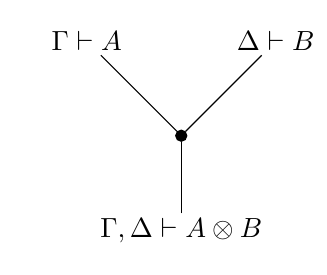
\begin{tikzpicture}
[inner sep=0.5mm,scale=0.6,auto,place/.style={circle,draw=blue!50,fill=blue!20,thick},
transition/.style={circle,draw=black,fill=black}]
\node (topl) at (-2,2) {$\Gamma \vdash A$};
\node (topr) at (2,2) {$\Delta \vdash B$};
\node (bottomm) at (0,-2) {$\Gamma, \Delta \vdash A \otimes B$};
\node (o) at (0,0) [transition] {};
\draw (bottomm) -- (o);
\draw (o) -- (topr);
\draw (o) -- (topl);
\end{tikzpicture}
&
\AxiomC{$\Gamma \vdash A$} \AxiomC{$\Delta \vdash B$}
\BinaryInfC{$\Gamma, \Delta \vdash A \otimes B$}
\DisplayProof
\end{tabular}
\end{center}
Leaves are presented in the sequent calculus notation with an empty numerator.

\begin{definition} A \emph{proof} is a pre-proof together with a compatible labelling of vertices by deduction rules. The list of deduction rules is given in the first column of \eqref{deduction_rule_ax} -- \eqref{deduction_rule_right1}. A labelling is \emph{compatible} if at each vertex, the sequents labelling the incident edges match the format displayed in the deduction rule.
\end{definition}

In all deduction rules, the sets $\Gamma$ and $\Delta$ may be empty and, in particular, the promotion rule may be used with an empty premise. In the promotion rule, ${!} \Gamma$ stands for a list of formulas each of which is preceeded by an exponential modality, for example ${!}A_1,\ldots, {!}A_n$. The diagrams on the right are string diagrams and should be ignored until Section \ref{section:diagrammatics}. In particular they are \emph{not} the trees associated to proofs.

% The linear logic of Girard \cite{girard_llogic, mellies} is a refinement of classical logic in which the contraction rule is restricted to formulas that are prefixed with a new unary connective ${!}$ called the exponential modality. A hypothesis ${!} A$ may be used in a proof infinitely many times as in classical logic, but a bare formula $A$ may only be used once\footnote{To an algebraist, this may sound as strange as an admonition to only use Nakayama's lemma once a day. After all, isn't the truth endlessly reusable? In reply, we would ask the reader to consider again the interpretation of the proof $\gamma$ in \eqref{integrate_against_a_proof} as a function mapping input proofs to output proofs. The act of computing these outputs is a physical process, whether it takes place in a machine or a human mind, and it involves the allocation and deallocation of finite resources. The insight of Girard with linear logic is that far from being implementation or engineering details, these acts of allocation and deallocation are in fact logical, and of fundamental importance.} (the proof is \emph{linear} in $A$). The other connectives are also refined, for instance $\Rightarrow$ is refined to a linear implication $\multimap$, with the former being recovered from the latter by the translation $A \Rightarrow B = {!} A \multimap B$.

% We consider propositional intuitionistic linear logic without additives (henceforth referred to simply as \emph{linear logic}). The adjective \emph{intuitionistic} means that the right hand side of a sequent is constrained to have precisely one formula, while \emph{propositional} means that we omit quantifiers.\footnote{The additives may be included in the obvious way, we omit them simply because our examples do not involve them. At the moment we do not understand quantifiers.} 

% Axiom rule
\begin{center}
\begin{tabular}{ >{\centering}m{6cm} >{\centering}m{6cm} >{\centering}m{2cm}}
\AxiomC{}
\LeftLabel{(Axiom): }
\UnaryInfC{$A \vdash A$}
\DisplayProof
&
\begin{tikzpicture}[scale=0.6,auto]
\node (top) at (0,1) {$A$};
\node (bottom) at (0,-1) {$A$};
\draw (bottom) -- (top);
\end{tikzpicture}
&
\tagarray{\label{deduction_rule_ax}}
\end{tabular}
\end{center}

% Exchange rule ======
\begin{center}
\begin{tabular}{ >{\centering}m{6cm} >{\centering}m{6cm} >{\centering}m{2cm}}
\AxiomC{$\Gamma, A, B, \Delta \vdash C$}
\LeftLabel{(Exchange): }
\UnaryInfC{$\Gamma, B, A, \Delta \vdash C$}
\DisplayProof
&
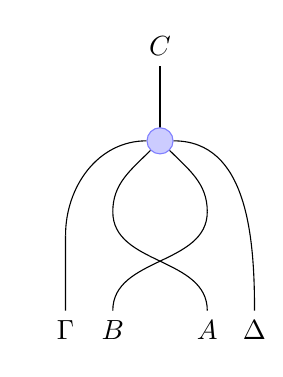
\begin{tikzpicture}[scale=0.6,auto]
\node (gamma) at (-2,-4) {$\Gamma$};
\node (a) at (1,-4) {$A$};
\node (b) at (-1,-4) {$B$};
\node (delta) at (2,-4) {$\Delta$};
\node (top) at (0,2) {$C$};
\draw (0,0) -- (top);
\bluenode (o) at (0,0) {};
\draw[out=90,in=180] (-2,-2) to (o);
\draw (gamma) -- (-2,-2);
\draw[out=90,in=225] (-1,-1.5) to (o);
\draw[out=90,in=270] (a) to (-1,-1.5);
\draw[out=90,in=315] (1,-1.5) to (o);
\draw[out=90,in=270] (b) to (1,-1.5);
\draw[out=90,in=0] (delta) to (o);
\end{tikzpicture}
&
\tagarray{\label{deduction_rule_ex}}
\end{tabular}
\end{center}

% Cut rule ======
\begin{center}
\begin{tabular}{ >{\centering}m{6cm} >{\centering}m{6cm} >{\centering}m{2cm}}
\AxiomC{$\Gamma \vdash A$} 
\AxiomC{$\Delta', A, \Delta \vdash B$}
\LeftLabel{(Cut): }
\RightLabel{\scriptsize cut}
\BinaryInfC{$\Delta',\Gamma, \Delta \vdash B$}
\DisplayProof
&
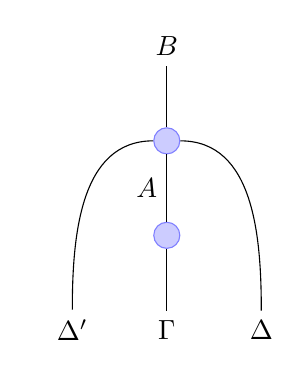
\begin{tikzpicture}[scale=0.6,auto]
\node (top) at (0,4) {$B$};
\node (bottom_mid) at (0,-2) {$\Gamma$};
\node (bottomr) at (2,-2) {$\Delta$};
\node (bottoml) at (-2,-2) {$\Delta'$};
\bluenode (1) at (0,0) {};
\bluenode (2) at (0,2) {};
\draw (bottom_mid) -- (1);
\draw[out=90,in=270] (1) to node {$A$} (2);
\draw[out=90,in=0] (bottomr) to (2);
\draw[out=90,in=180] (bottoml) to (2);
\draw (2) -- (top);
\end{tikzpicture}
&
\tagarray{\label{deduction_rule_cut}}
\end{tabular}
\end{center}


% Right tensor ======
\begin{center}
\begin{tabular}{ >{\centering}m{6cm} >{\centering}m{6cm} >{\centering}m{2cm}}
\AxiomC{$\Gamma \vdash A$} \AxiomC{$\Delta \vdash B$}
\LeftLabel{(Right $\otimes$): }
\RightLabel{\scriptsize $\otimes$-$R$}
\BinaryInfC{$\Gamma, \Delta \vdash A \otimes B$}
\DisplayProof
&
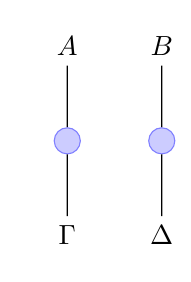
\begin{tikzpicture}[scale=0.6,auto]
\node (topl) at (-1,2) {$A$};
\node (topr) at (1,2) {$B$};
\node (bottoml) at (-1,-2) {$\Gamma$};
\node (bottomr) at (1,-2) {$\Delta$};
\bluenode (l) at (-1,0) {};
\bluenode (r) at (1,0) {};
\draw (bottoml) -- (l);
\draw (l) -- (topl);
\draw (bottomr) -- (r);
\draw (r) -- (topr);
\end{tikzpicture}
&
\tagarray{\label{deduction_rule_righttensor}}
\end{tabular}
\end{center}

% Left tensor ======
\begin{center}
\begin{tabular}{ >{\centering}m{6cm} >{\centering}m{6cm} >{\centering}m{2cm}}
\AxiomC{$\Gamma, A, B, \Delta \vdash C$}
\LeftLabel{(Left $\otimes$): }
\RightLabel{\scriptsize $\otimes$-$L$}
\UnaryInfC{$\Gamma, A \otimes B, \Delta \vdash C$}
\DisplayProof
&
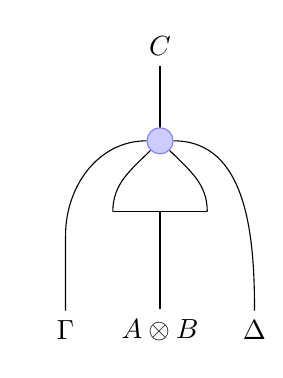
\begin{tikzpicture}[scale=0.6,auto]
\node (gamma) at (-2,-4) {$\Gamma$};
\node (mid) at (0,-4) {$A \otimes B$};
\node (delta) at (2,-4) {$\Delta$};
\node (top) at (0,2) {$C$};
\draw (0,0) -- (top);
\bluenode (o) at (0,0) {};
\draw[out=90,in=180] (-2,-2) to (o);
\draw (gamma) -- (-2,-2);
\draw (-1,-1.5) to (1,-1.5);
\draw[out=90,in=225] (-1,-1.5) to (o);
\draw (mid) to (0,-1.5);
\draw[out=90,in=315] (1,-1.5) to (o);
\draw[out=90,in=0] (delta) to (o);
\end{tikzpicture}
&
\tagarray{\label{deduction_rule_lefttensor}}
\end{tabular}
\end{center}

% Right Hom ======
\begin{center}
\begin{tabular}{ >{\centering}m{6cm} >{\centering}m{6cm} >{\centering}m{2cm}}
\AxiomC{$A, \Gamma \vdash B$}
\LeftLabel{(Right $\multimap$): }
\RightLabel{\scriptsize $\multimap R$ }
\UnaryInfC{$\Gamma \vdash A \multimap B$}
\DisplayProof
&
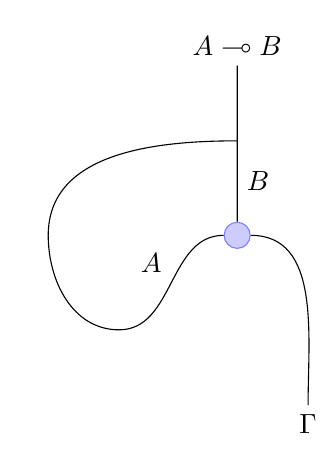
\begin{tikzpicture}[scale=0.6,auto]
\node (topr) at (1,4) {$A \multimap B$};
\bluenode (o) at (1,0) {};
\node (gamma) at (2.5,-4) {$\Gamma$};
\draw[out=90,in=0] (gamma) to (o);
\draw[out=0,in=180] (-1.5,-2) to node {$A$} (o);
\draw[out=180,in=270] (-1.5,-2) to (-3,0);
\draw[out=90,in=180] (-3,0) to (1,2);
\draw (o) to node [swap] {$B$} (1,2);
\draw (1,2) to (topr);
\end{tikzpicture}
&
\tagarray{\label{deduction_rule_righthom}}
\end{tabular}
\end{center}

% Left Hom ======
\begin{center}
\begin{tabular}{ >{\centering}m{6cm} >{\centering}m{6cm} >{\centering}m{2cm}}
\AxiomC{$\Gamma \vdash A$} \AxiomC{$\Delta', B, \Delta \vdash C$}
\LeftLabel{(Left $\multimap$): }
\RightLabel{\scriptsize $\multimap L$ }
\BinaryInfC{$\Delta', \Gamma, A \multimap B, \Delta \vdash C$}
\DisplayProof
&
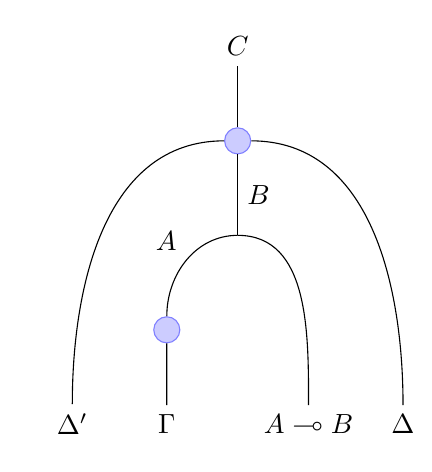
\begin{tikzpicture}[scale=0.6,auto]
\node (topr) at (0,2) {$C$};
\bluenode (q) at (-1.5,-4) {};
\bluenode (o) at (0,0) {};
\node (delta) at (3.5,-6) {$\Delta$};
\node (deltap) at (-3.5,-6) {$\Delta'$};
\node (gamma) at (-1.5, -6) {$\Gamma$};
\node (ab) at (1.5,-6) {$A \multimap B$};
\draw[out=90,in=0] (delta) to (o);
\draw[out=90,in=180] (deltap) to (o);
\draw (o) to (topr);
\draw[out=90,in=270] (0,-2) to node [swap] {$B$} (o);
\draw[out=90,in=270] (gamma) to (q);
\draw[out=90,in=180] (q) to node {$A$} (0,-2);
\draw[out=90,in=0] (ab) to (0,-2);
\end{tikzpicture}
&
\tagarray{\label{deduction_rule_lefthom}}
\end{tabular}
\end{center}

% Promotion ======
\begin{center}
\begin{tabular}{ >{\centering}m{6cm} >{\centering}m{6cm} >{\centering}m{2cm}}
\AxiomC{$! \Gamma \vdash A$}
\LeftLabel{(Promotion): }
\RightLabel{\scriptsize prom}
\UnaryInfC{$!\Gamma \vdash !A$}
\DisplayProof
&
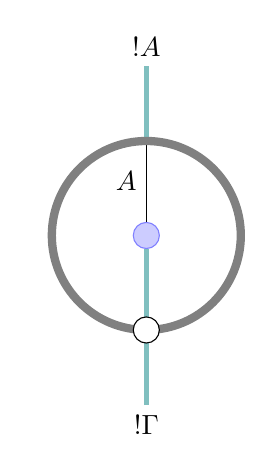
\begin{tikzpicture}[scale=0.6,auto]
\node (top) at (0,4) {$!A$};
\node (bottom) at (0,-4) {$!\Gamma$};
\bluenode (o) at (0,0) {};
\draw (o) to node {$A$} (0,2);
\drawbang (bottom) -- (0,-2);
\drawbang (0,2) -- (top);
\drawbang (0,-2) -- (o);
\drawprom (0,0) ellipse (2cm and 2cm);
\dernode (bottom) at (0,-2) {};
\end{tikzpicture}
&
\tagarray{\label{deduction_rule_prom}}
\end{tabular}
\end{center}

% Dereliction ======
\begin{center}
\begin{tabular}{ >{\centering}m{6cm} >{\centering}m{6cm} >{\centering}m{2cm}}
\AxiomC{$\Gamma, A, \Delta \vdash B$}
\LeftLabel{(Dereliction): }
\RightLabel{\scriptsize der}
\UnaryInfC{$\Gamma, !A, \Delta \vdash B$}
\DisplayProof
&
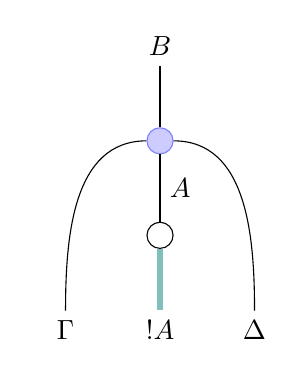
\begin{tikzpicture}[scale=0.6,auto]
\node (top) at (0,2) {$B$};
\bluenode (o) at (0,0) {};
\dernode (d) at (0,-2) {};
\node (gamma) at (-2, -4) {$\Gamma$};
\node (delta) at (2, -4) {$\Delta$};
\node (banga) at (0,-4) {$!A$};
\drawbang (banga) -- (d);
\draw (o) -- (top);
\draw[out=90,in=270] (d) to node [swap] {$A$} (o);
\draw[out=90,in=0] (delta) to (o);
\draw[out=90,in=180] (gamma) to (o);
\end{tikzpicture}
&
\tagarray{\label{deduction_rule_der}}
\end{tabular}
\end{center}

% Contraction ======
\begin{center}
\begin{tabular}{ >{\centering}m{6cm} >{\centering}m{6cm} >{\centering}m{2cm}}
\AxiomC{$\Gamma, !A, !A, \Delta \vdash B$}
\LeftLabel{(Contraction): }
\RightLabel{\scriptsize ctr}
\UnaryInfC{$\Gamma, !A, \Delta \vdash B$}
\DisplayProof
&
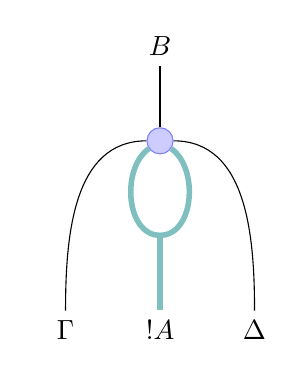
\begin{tikzpicture}[scale=0.6,auto]
\node (top) at (0,2) {$B$};
\bluenode (o) at (0,0) {};
\node (gamma) at (-2, -4) {$\Gamma$};
\node (delta) at (2, -4) {$\Delta$};
\node (banga) at (0,-4) {$!A$};
\drawbang (banga) -- (0,-2);
\draw (o) -- (top);
\drawbang[out=0,in=325] (0,-2) to (o);
\drawbang[out=180,in=215] (0,-2) to (o);
\draw[out=90,in=0] (delta) to (o);
\draw[out=90,in=180] (gamma) to (o);
\end{tikzpicture}
&
\tagarray{\label{deduction_rule_contr}}
\end{tabular}
\end{center}

% Weakening ======
\begin{center}
\begin{tabular}{ >{\centering}m{6cm} >{\centering}m{6cm} >{\centering}m{2cm}}
\AxiomC{$\Gamma, \Delta \vdash B$}
\LeftLabel{(Weakening): }
\RightLabel{\scriptsize weak}
\UnaryInfC{$\Gamma, !A, \Delta \vdash B$}
\DisplayProof
&
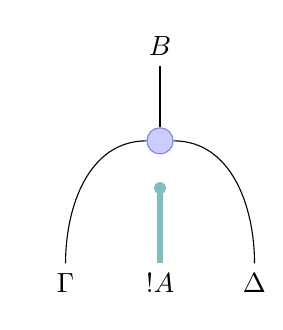
\begin{tikzpicture}[scale=0.6,auto]
\node (top) at (0,2) {$B$};
\bluenode (o) at (0,0) {};
\node (gamma) at (-2, -3) {$\Gamma$};
\node (delta) at (2, -3) {$\Delta$};
\node (banga) at (0,-3) {$!A$};
\drawbang (banga) -- (0,-1);
\draw (o) -- (top);
\draw[out=90,in=0] (delta) to (o);
\draw[out=90,in=180] (gamma) to (o);
\node[circle,draw=teal!50,fill=teal!50,inner sep=0.5mm] at (0,-1) {};
\end{tikzpicture}
&
\tagarray{\label{deduction_rule_weak}}
\end{tabular}
\end{center}

% Left 1 ======
\begin{center}
\begin{tabular}{ >{\centering}m{6cm} >{\centering}m{6cm} >{\centering}m{2cm}}
\AxiomC{$\Gamma, \Delta \vdash A$}
\LeftLabel{(Left $1$): }
\RightLabel{\scriptsize $1$-$L$}
\UnaryInfC{$\Gamma, 1, \Delta \vdash A$}
\DisplayProof
&
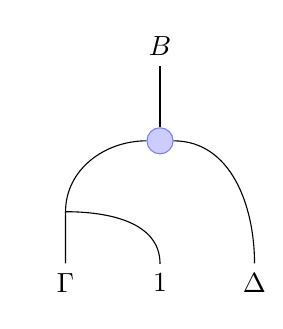
\begin{tikzpicture}[scale=0.6,auto]
\node (top) at (0,2) {$B$};
\bluenode (o) at (0,0) {};
\node (gamma) at (-2, -3) {$\Gamma$};
\node (delta) at (2, -3) {$\Delta$};
\node (one) at (0,-3) {$1$};
\draw (o) -- (top);
\draw (gamma) to (-2,-1.5);
\draw[out=90,in=180] (-2,-1.5) to (o);
\draw[out=90,in=0] (delta) to (o);
\draw[out=90,in=0] (one) to (-2,-1.5);
\end{tikzpicture}
&
\tagarray{\label{deduction_rule_left1}}
\end{tabular}
\end{center}

% Right 1 ======
\begin{center}
\begin{tabular}{ >{\centering}m{6cm} >{\centering}m{6cm} >{\centering}m{2cm}}
\AxiomC{}
\LeftLabel{(Right $1$): }
\RightLabel{\scriptsize $1$-$R$}
\UnaryInfC{$\vdash 1$}
\DisplayProof
&
\begin{tikzpicture}[scale=0.6,auto]
\node (top) at (0,1) {$1$};
\node (bottom) at (0,-1) {$1$};
\draw (bottom) -- (top);
\end{tikzpicture}
&
\tagarray{\label{deduction_rule_right1}}
\end{tabular}
\end{center}

\begin{example}\label{example:first_occur_2} For any formula $A$ let $\church{2}_A$ denote the proof \eqref{church_2_intro} from Section \ref{section:sketch}, which we repeat here for the reader's convenience:
\begin{center}
\AxiomC{}
\UnaryInfC{$A \vdash A$}
\AxiomC{}
\UnaryInfC{$A \vdash A$}
\AxiomC{}
\UnaryInfC{$A \vdash A$}
\RightLabel{\scriptsize$\multimap L$}
\BinaryInfC{$A, A \multimap A \vdash A$}
\RightLabel{\scriptsize$\multimap L$}
\BinaryInfC{$A, A \multimap A, A \multimap A \vdash A$}
\RightLabel{\scriptsize$\multimap R$}
\UnaryInfC{$A \multimap A, A \multimap A \vdash A \multimap A$}
\RightLabel{\scriptsize der}
\UnaryInfC{$!( A \multimap A ), A \multimap A \vdash A \multimap A$}
\RightLabel{\scriptsize der}
\UnaryInfC{$!( A \multimap A), !(A \multimap A) \vdash A \multimap $}
\RightLabel{\scriptsize ctr}
\UnaryInfC{$!( A \multimap A) \vdash A \multimap A$}
\RightLabel{\scriptsize$\multimap R$}
\UnaryInfC{$\vdash \inta_A$}
\DisplayProof
\qquad
\tagarray{\label{church_2_prooftree}}
\end{center}
We also write $\church{2}_A$ for the proof of ${!}( A \multimap A ) \vdash A \multimap A$ obtained by reading the above proof up to the penultimate line. For each integer $n \ge 0$ there is a proof $\church{n}_A$ of $\inta_A$ constructed along similar lines, see \cite[\S 5.3.2]{girard_llogic} and \cite[\S 3.1]{danos}.
\end{example}
%  Although the proof obviously has a structure similar to \eqref{church_2_prooftree_classic} notice that there is a conversion between $A \multimap A$ and its infinite version ${!}(A \multimap A)$, where the duplication occurs. 

In what sense is this proof an avatar of the number $2$? In the context of the $\lambda$-calculus we appreciated the relationship between the term $T$ and the number $2$ only after we saw how $T$ interacted with other terms $M$ by forming the function application $(T \, M)$ and then finding a normal form with respect to $\beta$-equivalence. 

The analogue of function application in linear logic is the cut rule. The analogue of $\beta$-equivalence is an equivalence relation on the set of proofs of any sequent, which we write as $\rho =_{cut} \delta$ and communicate by saying that $\rho$ and $\delta$ are \emph{equivalent under cut-elimination}. Next we describe how this equivalence relation  gives a dynamic meaning to the proof $\church{2}_A$, while postponing the actual definition of cut-elimination until Section \ref{section:cut_elim}.

\begin{example}\label{example:cutagainst2} Let $\pi$ be any proof of $A \vdash A$ and consider the proof 
\begin{equation}\label{cut_against_2_early}
\begin{mathprooftree}
\AxiomC{$\pi$}
\noLine\UnaryInfC{$\vdots$}
\def\extraVskip{5pt}
\noLine\UnaryInfC{$A \vdash A$}
\RightLabel{\scriptsize $\multimap R$}
\UnaryInfC{$\vdash A \multimap A$}
\RightLabel{\scriptsize prom}
\UnaryInfC{$\vdash {!}(A \multimap A)$}
\def\extraVskip{2pt}
\AxiomC{$\church{2}_A$}
\noLine\UnaryInfC{$\vdots$}
\def\extraVskip{5pt}
\noLine\UnaryInfC{$!(A \multimap A) \vdash A \multimap A$}
\def\extraVskip{2pt}
\RightLabel{\scriptsize cut}
\BinaryInfC{$\vdash A \multimap A$}
\end{mathprooftree}
\end{equation}
We write $\delta \l \rho$ for the cut rule applied with left branch $\rho$ and right branch $\delta$, and $\operatorname{prom}( \pi )$ for the left hand branch of \eqref{cut_against_2_early}, so that the whole proof is denoted $\church{2}_A \l \operatorname{prom}( \pi )$.

Intuitively, the promotion rule ``makes perennial'' the data of the proof $\pi$ and prepares it to be used more than once (that is, in a nonlinear way). This is related to the idea of \emph{storage} in the execution of programs on a physical system. The cut rule is logically the incarnation of Modus Ponens, and from the point of view of categorical semantics is the linguistic antecedent of composition. In the context of \eqref{cut_against_2_early} it plays the role of feeding the perennial version of $\pi$ as input to $\church{2}_A$. After our experience with the $\lambda$-term $T$ it is not a surprise that the above proof is equivalent under cut-elimination to
\begin{equation}\label{cut_against_2_early_3}
\begin{mathprooftree}
\AxiomC{$\pi$}
\noLine\UnaryInfC{$\vdots$}
\def\extraVskip{5pt}
\noLine\UnaryInfC{$A \vdash A$}
\def\extraVskip{2pt}
\AxiomC{$\pi$}
\noLine\UnaryInfC{$\vdots$}
\def\extraVskip{5pt}
\noLine\UnaryInfC{$A \vdash A$}
\def\extraVskip{2pt}
\RightLabel{\scriptsize cut}
\BinaryInfC{$A \vdash A$}
\RightLabel{\scriptsize $\multimap R$}
\UnaryInfC{$\vdash A \multimap A$}
\end{mathprooftree}
\end{equation}
which is essentially the square $\pi \l \pi$.
\end{example}

With $\pi$ playing the role of the term $M$ in Section \ref{section:lambda_calc}, we see the close analogy between the program $T$ of $\lambda$-calculus and the proof $\church{2}_A$ of linear logic, with the cut \eqref{cut_against_2_early} playing the role of $(T \, M)$ and cut-elimination the role of $\beta$-reduction. A beautiful and pregnant insight, which has driven much recent progress on the border of logic and computer science, is that \emph{proofs are algorithms}: using the cut rule and cut-elimination, proofs are revealed in the guise of finite, structured objects deterministically transforming inputs to outputs.
The task of the next several sections is to explain how these algorithms can be \emph{realised} in the context of symmetric closed monoidal categories with additional structure.

\begin{remark} The analogy between proofs and programs is made precise by the \emph{Curry-Howard correspondence} and its many variants \cite[\S 6.5]{selinger} which relates programs in the simply-typed $\lambda$-calculus (and its extensions) to proofs in intuitionistic logic (and its extensions) with cut-elimination playing the role of $\beta$-reduction. We will not go into details here, but there is a chain of embeddings
\[
\big\{\textup{Simply-typed $\lambda$-calculus}\big\} \hookrightarrow \big\{\textup{Intuitionistic logic}\big\} \hookrightarrow \big\{\textup{Linear logic}\big\}
\]
using which we can translate programs in the simply-typed $\lambda$-calculus into proofs of linear logic; see \cite[\S 5.1, \S 5.3]{girard_llogic} and \cite{lafont,abramsky,benton_etal}.
\end{remark}

% For example, if $A,B$ denote types in propositional intuitionistic logic, and $A^\circ, B^\circ$ the corresponding types in linear logic, then $(A \Rightarrow B)^\circ := (! A^\circ) \multimap B^\circ$ where for atoms $A$ we declare $A^\circ = A$. There is a corresponding translation of proofs of $\vdash A$ to proofs of $\vdash A^\circ$. The Church numeral $\church{2}_A$ is a $\lambda$-term of type $(A \rightarrow A) \rightarrow (A \rightarrow A)$ which corresponds to a proof in intuitionistic logic of the sequent $\vdash (A \Rightarrow A) \Rightarrow (A \Rightarrow A)$. If $A$ is atomic, the translation of this type to linear logic is $\inta_A' = {!}( {!}A \multimap A ) \multimap ({!}A \multimap A)$. Thus a Church numeral in the $\lambda$-calculus determines a proof of $\vdash \inta_A'$ not $\vdash \inta_A$ under this translation. However, this translation is not necessarily the most useful or economical one because of the over-use of exponentials \cite[\S 5.3]{girard_llogic}. For reasons of clarity we follow standard practice in using the ``linear logic version'' of the Church numeral $\church{2}_A$ in Example \ref{example:first_occur_2} above, rather than the literal translation.

\section{Semantics of linear logic}\label{section:diagrammatics}

\setlength{\epigraphwidth}{0.8\textwidth}
\epigraph{Denotational semantics originated in the work of Scott and Strachey (1971) and Scott (1976) as an attempt to interpret in a non-trivial way the quotient induced on $\lambda$-terms by $\beta$-equivalence. This amounts to finding an invariant of reduction, a question which may be extended to logical systems enjoying cut-elimination. Since its introduction, denotational semantics has proved to be an absolutely essential tool in computer science and proof theory, providing a wealth of information and insights into the nature of computation and formal proofs.}{P.~Boudes, D.~Mazza, L.~Tortora de Falco, \textit{An Abstract Approach to Stratification in Linear Logic}}

The structure of the set of proofs of a sequent $\Gamma \vdash A$ modulo equivalence under cut-elimination is quite complicated, and one way to understand this structure is to model it in simpler mathematical structures. These models are called \emph{semantics}. A \emph{categorical semantics} of linear logic \cite{mellies, blue_book} assigns to each formula $A$ an object $\den{A}$ of some category and to each proof of $\Gamma \vdash A$ a morphism $\den{\Gamma} \lto \den{A}$ in such a way that two proofs equivalent under cut-elimination are assigned the same morphism; these objects and morphisms are called \emph{denotations}. The connectives of linear logic become structure on the category of denotations, and compatibility with cut-elimination imposes identities relating these structures to one another.

In its general outlines the kind of structure imposed on the category of denotations is clear from the cut-elimination transformations themselves, but there are some subtleties; for a history of the development see \cite{mellies}. The upshot is that to define a categorical semantics the category of denotations must be a closed symmetric monoidal category equipped with a comonad, which is used to model the exponential modality \cite[\S 7]{mellies}. This is a refinement of the equivalence between simply-typed $\lambda$-calculus and cartesian closed categories due to Lambek and Scott \cite{lambek}. 

In this section we present the vector space semantics of linear logic, following \cite[p.5]{hyland}. The denotations of formulas are (infinite-dimensional) vector spaces, and the denotations of proofs are linear maps. We begin by explaining the denotations of formulas in Section \ref{section:denote_formula}. The denotations of proofs is trickier, and we first review the language of string diagrams in Section \ref{section:stringdiag} before giving the semantics and examples in Section \ref{section:vector_space_sem}.

\begin{remark} The first semantics of linear logic were the coherence spaces of Girard \cite[\S 3]{girard_llogic} which are a refined form of Scott's model of the $\lambda$-calculus. Models of full linear logic with negation involve the $\star$-autonomous categories of Barr \cite{barr_auto,barr_acc,barr_autolin} and the extension to include quantifiers involves indexed monoidal categories \cite{seely}.
\end{remark}

\subsection{Denotations of formulas}\label{section:denote_formula}

Let $k$ be an algebraically closed field of characteristic zero. All vector spaces are $k$-vector spaces and $\cat{V}$ denotes the category of vector spaces (not necessarily finite-dimensional) whose tensor product $\otimes_k$ is written $\otimes$.

For a vector space $V$ let ${!} V$ denote the cofree cocommutative coalgebra generated by $V$. We will discuss the explicit form of this coalgebra in the next section; for the moment it is enough to know that it exists, is determined up to unique isomorphism, and there is a linear map $d: {!} V \lto V$ which is universal.

\begin{definition}\label{defn:denotation_objects} The \emph{denotation} $\den{A}$ of a formula $A$ is defined inductively as follows:
\begin{itemize}
\item The propositional variables $x, y, z, \ldots$ are assigned chosen finite-dimensional vector spaces $\den{x}, \den{y}, \den{z}, \ldots$;
\item $\den{1} = k$;
\item $\den{A \otimes B} = \den{A} \otimes \den{B}$;
\item $\den{A \multimap B} = \den{A} \multimap \den{B}$ which is notation for $\Hom_k(\den{A}, \den{B})$;
\item $\den{!A} = {!} \den{A}$.
\end{itemize}
The denotation of a group of formulas $\Gamma = A_1,\ldots,A_n$ is their tensor product
\[
\den{\Gamma} = \den{A_1} \otimes \cdots \otimes \den{A_n}\,.
\]
If $\Gamma$ is empty then $\den{\Gamma} = k$.
\end{definition}

% We continue with the Church numeral $\church{2}_A$ as our motivating example:

%\begin{remark} This non-linearity can be traced to the duplication of terms that takes place during $\beta$-reduction. To see this, notice how in \eqref{eq:beta_reduc_dup} a single occurrence of $M$ on the left becomes a pair of $M$'s on the right, so that during the substitution process the term $M$ is duplicated. This duplication is not linear, because in general there is no linear map
%\begin{equation}\label{eq:dup_map_end}
%\End_k(V) \lto \End_k(V) \otimes \End_k(V)
%\end{equation}
%sending $\alpha$ to $\alpha \otimes \alpha$ for all $\alpha$, where $\End_k(V)$ denotes the space of linear maps $V \lto V$. One way to represent $T_{typed}$ as a linear map is to replace $\End_k(V)$ by the universal vector space over it which \emph{is} equipped with a duplication map satisfying some natural axioms; this is the universal cocommutative coalgebra ${!} \End_k(V)$. Using this coalgebra we may associate to $T_{typed}$ a linear map from which the non-linear map $\alpha \mapsto \alpha^2$ may be recovered; see Example \ref{example:denotation_2} below and Lemma \ref{lemma:nonlinear_recover}. %In the introduction we emphasised a link between duplication and infinity, and this will become clearer once we have understood the link between duplication and non-linearity, see Remark \ref{remark:dup_infinite} below.

%But we are getting ahead of ourselves. The first step is to reformulate the $\lambda$-calculus in terms of classical logic, then we identify the part of the logic that is responsible for this duplication -- called the contraction rule -- and explain how the contraction rule is refined in linear logic in such a way as to lead naturally to the coalgebra ${!} \End_k(V)$.
%\end{remark}

\begin{example}\label{example:denotation_2}  Let $A$ be a formula whose denotation is $V = \den{A}$. Then from \eqref{defn:integers},
\[
\den{\inta_A} = \den{ {!}( A \multimap A) \multimap (A \multimap A)} = \Hom_k( {!} \End_k(V), \End_k(V) )\,.
\]
\end{example}

In order to fortify the reader for some technical material in the next section, let us give a preview of the essential features of the semantics:

\begin{example}\label{example:2_denotation_preview} Let $A$ be a formula and $V = \den{A}$. The denotation of the proof $\church{2}_A$ of $\vdash \inta_A$ from Example \ref{example:first_occur_2} will be a morphism
\begin{equation}\label{eq:2_as_comp_0}
\den{\church{2}_A}: k \lto \den{\inta_A} = \Hom_k( {!} \End_k(V), \End_k(V) )\,,
\end{equation}
or equivalently, a linear map ${!} \End_k(V) \lto \End_k(V)$. What is this linear map? It turns out (see Example \ref{example:church_2} below for details) that it is the composite
\begin{equation}\label{eq:2_as_comp}
\xymatrix@C+0.5pc{
{!} \End_k(V) \ar[r]^-{\Delta} & {!} \End_k(V) \otimes {!} \End_k(V) \ar[r]^-{d \otimes d} & \End_k(V)^{\otimes 2} \ar[r]^-{- \circ -} & \End_k(V)
}
\end{equation}
where $\Delta$ is the coproduct, $d$ is the universal map, and the last map is the composition. How to reconcile this linear map with the corresponding program in the $\lambda$-calculus, which has the meaning ``square the input function''? As we will explain below, for $\alpha \in \End_k( V )$ there is a naturally associated element $\vacu_\alpha \in {!} \End_k(V)$ with the property that
\[
\Delta \vacu_\alpha = \vacu_\alpha \otimes \vacu_\alpha, \qquad d \vacu_\alpha = \alpha\,.
\]
Then $\den{\church{2}_A}$ maps this element to
\begin{equation}\label{eq:2_deals_with_0}
\vacu_\alpha \longmapsto \vacu_\alpha \otimes \vacu_\alpha \longmapsto \alpha \otimes \alpha \longmapsto \alpha \circ \alpha\,.
\end{equation}
%For $n > 2$ the Church numeral $\church{n}$ has $n$ occurrences of the left $\multimap$ introduction rule, and so has as its leaves $n + 1$ uses of the axiom rule. The corresponding diagram uses the coproduct $n-1$ times, and feeds the results into $n$ derelictions.
This demonstrates how the coalgebra ${!} \End_k(V)$ may be used to encode nonlinear maps, such as squaring an endomorphism.
\end{example}

\subsection{Background on string diagrams and coalgebras}\label{section:stringdiag}

%The category of $k$-vector spaces has all the properties of a category of proof denotations described earlier, including the comonad ${!}$ given by taking cofree cocommutative coalgebras, so it is automatic that semantics of intuitionistic linear logic may be constructed within $\cat{V}$. 

In order to present the denotations of proofs in the vector space semantics we need to firstly present the language of string diagrams following Joyal and Street \cite{JSGoTCI,JSGoTCII,ladia,khovdia,mellies, mellies_dia} and secondly present some material on cofree coalgebras in order to give formulas for the promotion and dereliction rules.

%.\footnote{This is not as surprising as it might seem: although studying semantics of \emph{linear} logic using vector spaces is an natural thing to do, research has focused on full linear logic with negation. This is more complicated than the intuitionistic case, because types must be interpreted by self-dual objects and this leads to topological vector spaces \cite{barr_auto, barr_acc, blute,blute_scott,girard_coherentbanach,ehrhard, ehrhard_kothe}.  However these more sophisticated models have the disadvantage that it is inconvenient to write down denotations of proofs, which is why for this introduction we stick to the intuitionistic case. See Remark \ref{remark_otherpromotion} for more on the existing literature.} 

%.\footnote{One style of string diagrams, called \emph{proof-nets}, were introduced by Girard and have been fundamental to linear logic since the beginning of the subject \cite{girard_llogic}.}

Let $\cat{V}$ denote the category of $k$-vector spaces (not necessarily finite dimensional). Then $\cat{V}$ is symmetric monoidal and for each object $V$ the functor $V \otimes -$ has a right adjoint
\[
V \multimap - := \Hom_k(V, -)\,.
\]
In addition to the usual diagrammatics of a symmetric monoidal category, we draw the evaluation map $V \otimes (V \multimap W) \lto W$ as
\begin{equation}\label{eq:diagram_eval_map}
\begin{tikzpicture}[scale=0.4,auto,baseline=(current  bounding  box.center)]
\node (topr) at (0,3) {$W$};
\coordinate (o) at (0,0) {};
\node (bottoml) at (-3,-4) {$V$};
\node (bottomr) at (3,-4) {$V \multimap W$};
\draw[out=90,in=180] (bottoml) to (o);
\draw[out=90,in=0] (bottomr) to (o);
\draw (o) to (topr);
\end{tikzpicture}
\qquad\qquad
v \otimes \psi \mapsto \psi(v)\,.
\end{equation}
The adjoint $Y \lto X \multimap Z$ of a morphism $\phi: X \otimes Y \lto Z$ is depicted as follows:\footnote{This is somewhat against the spirit of the diagrammatic calculus, since the loop labelled $X$ is not ``real'' and is only meant as a ``picture'' to be placed at a vertex between a strand labelled $Y$ and a strand labelled $X \multimap Z$. This should not cause confusion, because we will never manipulate this strand on its own. The idea is that if $X$ were a finite-dimensional vector space, so that $X \multimap Z \cong X^{\vee} \otimes Z$, the above diagram would be absolutely valid, and we persist with the same notation even when $X$ is not dualisable. In our judgement the clarity achieved by this slight cheat justifies a little valour in the face of correctness.}
\begin{equation}\label{eq:diagram_adjoint_of_map}
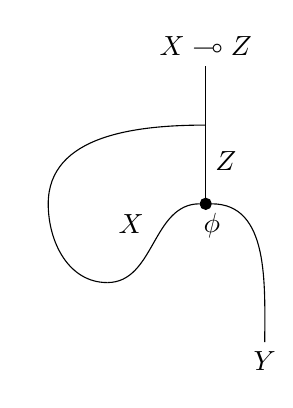
\begin{tikzpicture}[scale=0.5,auto,baseline=(current  bounding  box.center)]
\node (topr) at (1,4) {$X \multimap Z$};
\mapnode (o) at (1,0) {};
\node [below] at (o.east) {$\phi$};
\node (gamma) at (2.5,-4) {$Y$};
\draw[out=90,in=0] (gamma) to (o);
\draw[out=0,in=180] (-1.5,-2) to node {$X$} (o);
\draw[out=180,in=270] (-1.5,-2) to (-3,0);
\draw[out=90,in=180] (-3,0) to (1,2);
\draw (o) to node [swap] {$Z$} (1,2);
\draw (1,2) to (topr);
\end{tikzpicture}
\qquad
y \mapsto \{ x \mapsto \phi( x \otimes y ) \}\,.
\end{equation}
Next we present the categorical construct corresponding to the exponential modality in terms of an adjunction, following Benton \cite{benton}, see also \cite[\S 7]{mellies}. Let $\cat{C}$ denote the category of counital, coassociative, cocommutative coalgebras in $\cat{V}$. In this paper whenever we say \emph{coalgebra} we mean an object of $\cat{C}$. This is a symmetric monoidal category in which the tensor product (inherited from $\cat{V}$) is cartesian, see \cite[Theorem 6.4.5]{sweedler}, \cite{barr} and \cite[\S 6.5]{mellies}. 

By results of Sweedler \cite[Chapter 6]{sweedler} the forgetful functor $L: \cat{C} \lto \cat{V}$ has a right adjoint $R$ and we set ${!} = L \circ R$, as in the following diagram:\footnote{The existence of a right adjoint to the forgetful functor can also be seen to hold more generally as a consequence of the adjoint functor theorem \cite{barr}.}
\[
\xymatrix@C+3pc{
\cat{C}\ar@<0.7ex>[r]^-{L} & \cat{V} \ar@<0.7ex>[l]^-{R}
}
\qquad
! = L \circ R\,.
\]
Both $L$ and its adjoint $R$ are monoidal functors.

For each $V$ there is a coalgebra $! V$ and a counit of adjunction $d: {!} V \lto V$. Since this map will end up being the interpretation of the dereliction rule in linear logic, we refer to it as the \emph{dereliction map}. In string diagrams it is represented by an empty circle. Although it is purely decorative, it is convenient to represent coalgebras in string diagrams drawn in $\cat{V}$ by thick lines, so that for ${!} V$ the dereliction, coproduct and counit are drawn respectively as follows:
\begin{equation}\label{eq:coalgebra_maps}
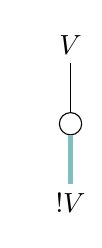
\begin{tikzpicture}[scale=0.5,auto,inner sep=1mm,baseline=(current  bounding  box.center)]
\node (top) at (0,2) {$V$};
\dernode (d) at (0,0) {};
\node (banga) at (0,-2) {$!V$};
\drawbang (banga) -- (d);
\draw (d) -- (top);
\end{tikzpicture}
\qquad\qquad\qquad
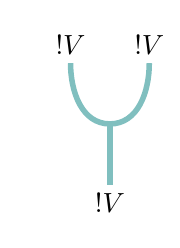
\begin{tikzpicture}[scale=0.5,auto,inner sep=1mm,baseline=(current  bounding  box.center)]
\node (topl) at (-1,2) {${!} V$};
\node (topr) at (1,2) {${!} V$};
\coordinate (d) at (0,0);
\node (banga) at (0,-2) {$!V$};
\drawbang (banga) -- (d);
\drawbang[out=0,in=270] (d) to (topr);
\drawbang[out=180,in=270] (d) to (topl);
\end{tikzpicture}
\qquad\qquad\qquad
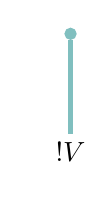
\begin{tikzpicture}[scale=0.5,auto,inner sep=1mm,baseline=(current  bounding  box.center)]
\node (banga) at (0,-2) {$!V$};
\node[circle,draw=teal!50,fill=teal!50,inner sep=0.5mm] (blah) at (0,1) {};
\drawbang (banga) -- (blah);
\end{tikzpicture}
\end{equation}
In this paper our string diagrams involve both $\cat{V}$ and $\cat{C}$ and our convention is that white regions represent $\cat{V}$ and gray regions stand for $\cat{C}$. A standard way of representing monoidal functors between monoidal categories is using coloured regions \cite[\S 5.7]{mellies}. The image under $L$ of a morphism $\alpha: C_1 \lto C_2$ in $\cat{C}$ is drawn as a vertex in a grey region embedded into a white region. The image of a morphism $\gamma: V_1 \lto V_2$ under $R$ is drawn using a white region embedded in a gray plane. For example, the diagrams representing $L(\alpha), R(\gamma)$ and ${!} \gamma = LR(\gamma)$ are respectively
\begin{center}
\begin{tikzpicture}
[inner sep=0.5mm,scale=0.6,auto,place/.style={circle,draw=blue!50,fill=blue!20,thick},
transition/.style={circle,draw=black,fill=black}]
\node (vtop) at (0,4.5) {$L C_2$};
\node (bottom) at (0,-4.5) {$L C_1$};
\drawbang (top) to (vtop);
\coordinate (bottom_c) at (0,-3);
\drawbang (bottom) to (bottom_c);
\coordinate (top_c) at (0,3);
\draw[color=gray, line width=3pt, fill=gray!20] (0,0) ellipse (2cm and 3cm);
\node (o) at (0,0) [transition] {};
\node [right] at (o.east) {$\alpha$};
\draw (o) to node [swap] {$C_2$} (top_c);
\draw (bottom_c) to node [swap] {$C_1$} (o);
\draw[color=gray, line width=3pt] (0,0) ellipse (2cm and 3cm);
\end{tikzpicture}
\qquad \qquad
\begin{tikzpicture}
[inner sep=0.5mm,scale=0.6,auto,place/.style={circle,draw=blue!50,fill=blue!20,thick},
transition/.style={circle,draw=black,fill=black}]
\draw[color=white,fill=gray!20] (-3,-4.1) rectangle (3,4.1);
\node (vtop) at (0,4.5) {$R V_2$};
\node (bottom) at (0,-4.5) {$R V_1$};
\draw (top) to (vtop);
\coordinate (bottom_c) at (0,-3);
\draw (bottom) to (bottom_c);
\coordinate (top_c) at (0,3);
\draw[color=gray, line width=3pt, fill=white] (0,0) ellipse (2cm and 3cm);
\node (o) at (0,0) [transition] {};
\node [right] at (o.east) {$\gamma$};
\draw (o) to node [swap] {$V_2$} (top_c);
\draw (bottom_c) to node [swap] {$V_1$} (o);
\draw[color=gray, line width=3pt] (0,0) ellipse (2cm and 3cm);
\end{tikzpicture}
\qquad \qquad
\begin{tikzpicture}
[inner sep=0.5mm,scale=0.6,auto,place/.style={circle,draw=blue!50,fill=blue!20,thick},
transition/.style={circle,draw=black,fill=black}]
\node (vtop) at (0,4.5) {${!} V_2 = LR V_2$};
\node (bottom) at (0,-4.5) {${!} V_1 = LR V_1$};
\coordinate (top_c) at (0,3);
\coordinate (bottom_c) at (0,-3);
\drawbang (top) to (vtop);
\drawbang (bottom) to (bottom_c);
\draw[color=gray, line width=3pt, fill=gray!20] (0,0) ellipse (3cm and 3.2cm);
\draw[color=gray, line width=3pt, fill=white] (0,0) ellipse (2.5cm and 1.2cm);
\node (o) at (0,0) [transition] {};
\node [right] at (o.east) {$\gamma$};
\draw (o) to (0,1.2);
\draw (o) to (0,-1.2);
\draw (0,1.2) to node [swap] {$RV_2$} (0,3.2);
\draw (0,-3.2) to node [swap] {$RV_1$} (0,-1.2);
\draw[color=gray, line width=3pt] (0,0) ellipse (3cm and 3.2cm);
\draw[color=gray, line width=3pt] (0,0) ellipse (2.5cm and 1.2cm);
\end{tikzpicture}
\end{center}
The adjunction between $R$ and $L$ means that for any coalgebra $C$ and linear map $\phi: C \lto V$ there is a unique morphism of coalgebras $\Phi : C \lto {!}V$ making
\begin{equation}\label{eq:defining_philift}
\xymatrix@C+1.5pc@R+1.5pc{
C \ar[r]^-{\phi}\ar[dr]_-{\Phi} & V\\
& {!}V \ar[u]_-{d}
}
\end{equation}
commute. The lifting $\Phi$ may be constructed as the unit followed by ${!} \phi$,
\[
\Phi := \xymatrix@C+2pc{ C \ar[r] & {!} C \ar[r]^-{{!} \phi} & {!} V}
\]
and since we also use an empty circle to denote the unit $C \lto {!} C$, this has the diagrammatic representation given on the right hand side of the following diagram. The left hand side is a convenient abbreviation for this morphism, that is, for the lifting $\Phi$:
% Promotion ======
\begin{equation}\label{eq:abbrev_for_prom}
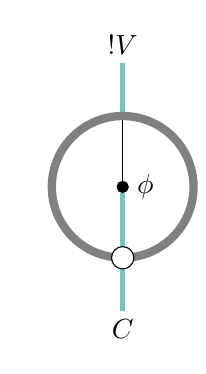
\begin{tikzpicture}[scale=0.6,auto,inner sep=1mm, baseline=(current  bounding  box.center)]
\node (top) at (0,3) {$!V$};
\node (bottom) at (0,-3) {$C$};
\mapnode (o) at (0,0) {};
\node [right] at (o.east) {$\phi$};
\draw (o) to (0,2);
\drawbang (bottom) -- (0,-1.5);
\drawbang (0,1.5) -- (top);
\drawbang (0,-1.5) -- (o);
\drawprom (0,0) ellipse (1.5cm and 1.5cm);
\dernode (bottom) at (0,-1.5) {};
\end{tikzpicture}
\qquad := \qquad
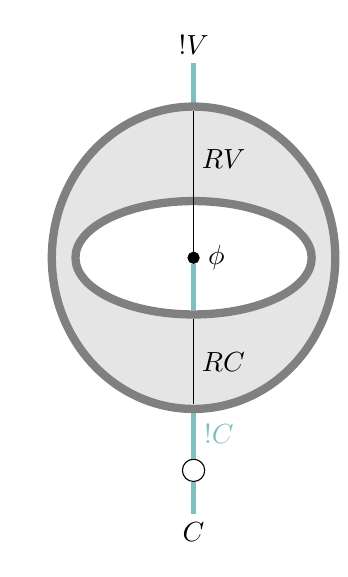
\begin{tikzpicture}[scale=0.6,auto,inner sep=1mm,baseline=(current  bounding  box.center)]
\node (vtop) at (0,4.5) {${!} V$};
\node (bottom) at (0,-5.8) {$C$};
\coordinate (top_c) at (0,3);
\coordinate (bottom_c) at (0,-3.2);
\drawbang (top_c) to (vtop);
\dernode (bottomd) at (0,-4.5) {};
\drawbang (bottomd) to node [swap] {${!} C$} (bottom_c);
\drawbang (bottom) to (bottomd);
\draw[color=gray, line width=3pt, fill=gray!20] (0,0) ellipse (3cm and 3.2cm);
\draw[color=gray, line width=3pt, fill=white] (0,0) ellipse (2.5cm and 1.2cm);
\mapnode (o) at (0,0) {};
\node [right] at (o.east) {$\phi$};
\draw (o) to (0,1.2);
\drawbang (o) to (0,-1.1);
\draw (0,1.1) to node [swap] {$RV$} (0,3.1);
\draw (0,-3.1) to node [swap] {$RC$} (0,-1.3);
\end{tikzpicture}
\end{equation}
We follow the logic literature in referring to the grey circle denoting the induced map $\Phi$ as a \emph{promotion box}. Commutativity of \eqref{eq:defining_philift} is expressed by the identity
\begin{equation}\label{eq:prom_cancel_der}
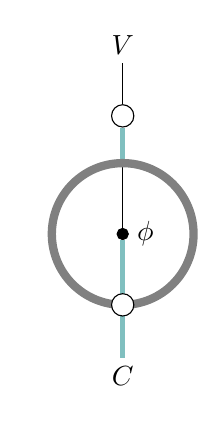
\begin{tikzpicture}[scale=0.6,auto,inner sep=1mm,baseline=(current  bounding  box.center)]
\node (top) at (0,4) {$V$};
\dernode (altop) at (0,2.5) {};
\node (bottom) at (0,-3) {$C$};
\mapnode (o) at (0,0) {};
\node [right] at (o.east) {$\phi$};
\draw (o) to (0,2);
\drawbang (bottom) -- (0,-1.5);
\drawbang (0,1.5) -- (altop);
\draw (altop) -- (top);
\drawbang (0,-1.5) -- (o);
\drawprom (0,0) ellipse (1.5cm and 1.5cm);
\dernode (bottom) at (0,-1.5) {};
\end{tikzpicture}
\qquad = \qquad
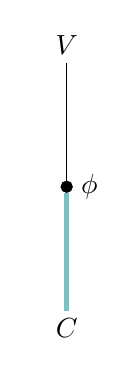
\begin{tikzpicture}[scale=0.6,auto,inner sep=1mm,baseline=(current  bounding  box.center)]
\node (top) at (0,3) {$V$};
\node (bottom) at (0,-3) {$C$};
\mapnode (o) at (0,0) {};
\node [right] at (o.east) {$\phi$};
\drawbang (bottom) -- (o);
\draw (o) -- (top);
\end{tikzpicture}
\end{equation}
which says that dereliction annihilates with promotion boxes.

The coalgebra ${!} V$ and the dereliction map ${!} V \lto V$ satisfy a universal property and are therefore unique up to isomorphism. However, to actually write down the denotations of proofs, we will need the more explicit construction which follows from the work of Sweedler \cite{sweedler} and is spelt out in \cite{murfet_coalg}. If $V$ is finite-dimensional then
\begin{equation}\label{eq:presentation_intro}
{!} V = \bigoplus_{P \in V} \Sym_P(V)
\end{equation}
where $\Sym_P(V) = \Sym(V)$ is the symmetric coalgebra. If $e_1,\ldots,e_n$ is a basis for $V$ then as a vector space $\Sym(V) \cong k[e_1,\ldots,e_n]$. The notational convention in \cite{murfet_coalg} is to denote, for elements $\nu_1,\ldots,\nu_s \in V$, the corresponding tensor in $\Sym_P(V)$ using kets
\begin{equation}\label{eq:ket_notation}
\ket{\nu_1,\ldots,\nu_s}_P := \nu_1 \otimes \cdots \otimes \nu_s \in \Sym_P(V)\,.
\end{equation}
And in particular, the identity element of $\Sym_P(V)$ is denoted by a vacuum vector
\begin{equation}\label{eq:vacuum}
\vacu_P := 1 \in \Sym_P(V)\,.
\end{equation}
We remark that if $\nu = 0$ then $\ket{\nu}_P = 0$ is the zero vector, which is distinct from $\vacu_P = 1$. To avoid unwieldy notation we sometimes write $\nu_1 \otimes \cdots \otimes \nu_s \cdot \vacu_P$ for $\ket{\nu_1,\ldots,\nu_s}_P$. With this notation the universal map $d: {!} V \lto V$ is defined by
\[
d \vacu_P = P, \quad d\ket{\nu}_P = \nu, \quad d\ket{\nu_1,\ldots,\nu_s}_P = 0 \quad s > 1\,.
\]
The coproduct on ${!} V$ is defined by
\begin{equation}\label{eq:lc_coalgebra_1}
\Delta \ket{ \nu_1, \ldots, \nu_s }_P = \sum_{I \subseteq \{ 1, \ldots, s \}} \ket{ \nu_I }_P \otimes \ket{ \nu_{I^c} }_P
\end{equation}
where $I$ ranges over all subsets including the empty set, for a subset $I = \{ i_1, \ldots, i_p \}$ we denote by $\nu_I$ the sequence $\nu_{i_1},\ldots,\nu_{i_p}$, and $I^c$ is the complement of $I$. In particular
\[
\Delta \vacu_P = \vacu_P \otimes \vacu_P\,.
\]
The counit ${!} V \lto k$ is defined by $\vacu_P \mapsto 1$ and $\ket{\nu_1,\ldots,\nu_s}_P \mapsto 0$ for $s > 0$.

When $V$ is infinite-dimensional we may define ${!} V$ as the direct limit over the coalgebras ${!} W$ for finite-dimensional subspaces $W \subseteq V$. These are sub-coalgebras of ${!} V$, and we may therefore use the same notation as in \eqref{eq:ket_notation} to denote arbitrary elements of ${!} V$. Moreover the coproduct, counit and universal map $d$ are given by the same formulas; see \cite[\S 2.1]{murfet_coalg}. A proof of the fact that the map $d: {!} V \lto V$ described above is universal among linear maps to $V$ from cocommutative coalgebras is given in \cite[Theorem 2.18]{murfet_coalg}, but as has been mentioned this is originally due to Sweedler \cite{sweedler}, see \cite[Appendix B]{murfet_coalg}.

To construct semantics of linear logic we also need an explicit description of liftings, as given by the next theorem which is \cite[Theorem 2.20]{murfet_coalg}. For a set $X$ the set of partitions of $X$ is denoted $\cat{P}_X$.

\begin{theorem}\label{theorem:describe_lifting} Let $W, V$ be finite-dimensional vector spaces and $\phi: {!}W \lto V$ a linear map. The unique lifting of $\phi$ to a morphism of coalgebras $\Phi: {!}W \lto {!}V$ is defined for vectors $P, \nu_1,\ldots,\nu_s \in W$ by
\begin{equation}\label{eq:describe_lift}
\Phi \ket{ \nu_1, \ldots, \nu_s }_P = \sum_{C \in \cat{P}_{\{1,\ldots,s\}}} \Big|\, \phi \ket{\nu_{C_{1}} }_P\,, \ldots \,, \phi \ket{ \nu_{C_{l}}}_P \Big\rangle_Q
\end{equation}
where $Q = \phi \vacu_P$ and $l$ denotes the length of the partition $C$.
\end{theorem}

%In constructing the vector space semantics of linear logic we will only encounter \eqref{eq:abbrev_for_prom} in the case where $C = {!} W$. %We will however give examples of lifting that involve other coalgebras, including the next example and in Appendix \ref{section:example_lifting}.

\begin{example}\label{example:lifting_trivial} The simplest example of a coalgebra is the field $k$. Any $P \in V$ determines a linear map $k \lto V$ whose lifting to a morphism of coalgebras $k \lto {!}V$ sends $1 \in k$ to the vacuum $\vacu_P$, as shown in the commutative diagram
\begin{equation}\label{eq:kaiwanxiao}
\xymatrix@C+2pc{
k \ar[r]^-{P} \ar@{.>}[dr]_-{\vacu_P} & V\\
& ! V \ar[u]_-{d}
}\,.
\end{equation}
Such liftings arise from promotions with empty premises, e.g. the proof\footnote{Incidentally, this proof helps explain why defining $\den{!A} = \Sym(\den{A})$ cannot lead to semantics of linear logic, since the denotation is a morphism of coalgebras $k \lto {!} \End_k(\den{A})$ whose composition with dereliction yields the map $k \lto \End_k( \den{A} )$ sending $1 \in k$ to the identity. But this map does not admit a lifting into the symmetric coalgebra, because it produces an infinite sum. However the symmetric coalgebra \emph{is} universal in a restricted sense and is (confusingly) sometimes also called a cofree coalgebra; see \cite[\S 4]{quillen}. For further discussion of the symmetric coalgebra in the context of linear logic see \cite{blute_fock,mellies2}.}
\begin{center}
\AxiomC{}
\UnaryInfC{$A \vdash A$}
\RightLabel{\scriptsize $\multimap R$}
\UnaryInfC{$\vdash A \multimap A$}
\RightLabel{\scriptsize prom}
\UnaryInfC{$\vdash {!}(A \multimap A)$}
\DisplayProof
\end{center}
\end{example}

\subsection{The vector space semantics}\label{section:vector_space_sem}

Recall from Definition \ref{defn:denotation_objects} the definition of $\den{A}$ for each formula $A$.

\begin{definition}\label{defn:denotation_morphism} The \emph{denotation} $\den{\pi}$ of a proof $\pi$ of $\Gamma \vdash B$ is a linear map $\den{\Gamma} \lto \den{B}$ defined by inductively assigning a string diagram to each proof tree; by the basic results of the diagrammatic calculus \cite{JSGoTCI} this diagram unambiguously denotes a linear map. The inductive construction is described by the second column in \eqref{deduction_rule_ax} -- \eqref{deduction_rule_weak}. 

In each rule we assume a morphism has already been assigned to each of the sequents in the numerator of the deduction rule. These inputs are represented by blue circles in the diagram, which computes the morphism to be assigned to the denominator. To simplify the appearance of diagrams, we adopt the convention that a strand labelled by a formula $A$ represents a strand labelled by the denotation $\den{A}$. In particular, a strand labelled with a sequence $\Gamma = A_1,\ldots,A_n$ represents a strand labelled by $\den{A_1} \otimes \cdots \otimes \den{A_n}$.
\end{definition}

Some comments:
\begin{itemize}
\item The diagram for the axiom rule \eqref{deduction_rule_ax} depicts the identity of $\den{A}$.
\item The diagram for the exchange rule \eqref{deduction_rule_ex} uses the symmetry $\den{B} \otimes \den{A} \lto \den{A} \otimes \den{B}$.
\item The diagram for the cut rule \eqref{deduction_rule_cut} depicts the composition of the two inputs.
\item The right tensor rule \eqref{deduction_rule_righttensor} depicts the tensor product of the two given morphisms, while the left tensor rule \eqref{deduction_rule_lefttensor} depicts the identity, viewed as a morphism between two strands labelled $\den{A}$ and $\den{B}$ and a single strand labelled $\den{A} \otimes \den{B}$.
\item The diagram for the right $\multimap$ rule \eqref{deduction_rule_righthom} denotes the adjoint of the input morphism as in \eqref{eq:diagram_adjoint_of_map} while the left $\multimap$ rule \eqref{deduction_rule_lefthom} uses the composition map from \eqref{eq:diagram_eval_map}.
\item The diagram for the promotion rule \eqref{deduction_rule_prom} depicts the lifting of the input to a morphism of coalgebras, as explained in \eqref{eq:abbrev_for_prom}.
\item The diagram for the dereliction rule \eqref{deduction_rule_der} depicts the composition of the input with the universal map out of the coalgebra ${!} V$. The notation for this map, and the maps in the contraction \eqref{deduction_rule_contr} and weakening rules \eqref{deduction_rule_weak} are as described in \eqref{eq:coalgebra_maps}.
\end{itemize}

\begin{remark} For this to be a valid semantics, two proofs related by cut-elimination must be assigned the same morphism. This is a consequence of the general considerations in \cite[\S 7]{mellies}. More precisely, $\cat{V}$ is a Lafont category \cite[\S 7.2]{mellies} and in the terminology of \emph{loc.cit.} the adjunction between $\cat{V}$ and $\cat{C}$ is a linear-nonlinear adjunction giving rise to a model of intuitionistic linear logic. For an explanation of how the structure of a symmetric monoidal category extrudes itself from the cut-elimination transformations, see \cite[\S 2]{mellies}.
\end{remark}

% Given the embedding of the simply-typed $\lambda$-calculus into linear logic, recalled in Appendix \ref{remark:embedding_intuit}, and the above construction of an interpretation of linear logic in the category $\cat{V}$ of $k$-vector spaces, we are finally in a position to answer Question \ref{question:lambda} in the positive. With patience, the reader may use the above to translate any program into a linear map. To explain how this works in practice, we go through the details of assigning a diagram and the corresponding linear map to the proof tree \eqref{church_2_prooftree} of the Church numeral $\church{2}_A$. 

\begin{example}\label{example:church_2} We convert the proof $\church{2}_A$ of \eqref{church_2_prooftree} to a diagram in stages, beginning with the leaves. Each stage is depicted in three columns: in the first is a partial proof tree, in the second is the diagram assigned to it by Definition \ref{defn:denotation_morphism}, and in the third is the explicit linear map which is the value of the diagram. 

Recall that a strand labelled $A$ actually stands for the vector space $V = \den{A}$, so for instance the first diagram denotes a linear map $V \otimes \End_k(V) \lto V$:
\begin{center}
% Church numeral 2 layer 1
\begin{tabular}{>{\centering}m{6cm} >{\centering}m{5cm} >{\centering}m{4cm}}
\AxiomC{}
\UnaryInfC{$A \vdash A$}
\AxiomC{}
\UnaryInfC{$A \vdash A$}
\RightLabel{\scriptsize$\multimap L$}
\BinaryInfC{$A, A \multimap A \vdash A$}
\DisplayProof
&
\begin{tikzpicture}[scale=0.3,auto]
\node (topr) at (0,2) {$A$};
\coordinate (o) at (0,0);
\node (delta) at (2.5,-4) {$A \multimap A$};
\node (left) at (-2.5, -4) {$A$};
\draw (o) to (topr);
\draw[out=90,in=180] (left) to (o);
\draw[out=90,in=0] (delta) to (o);
\end{tikzpicture}
&
$a \otimes \alpha \mapsto \alpha(a)$
\end{tabular}
\end{center}
\begin{center}
% Church numeral 2 layer 2
\begin{tabular}{>{\centering}m{6cm} >{\centering}m{5cm} >{\centering}m{4cm}}
\AxiomC{}
\UnaryInfC{$A \vdash A$}
\AxiomC{}
\UnaryInfC{$A \vdash A$}
\AxiomC{}
\UnaryInfC{$A \vdash A$}
\RightLabel{\scriptsize$\multimap L$}
\BinaryInfC{$A, A \multimap A \vdash A$}
\RightLabel{\scriptsize$\multimap L$}
\BinaryInfC{$A, A \multimap A, A \multimap A \vdash A$}
\DisplayProof
&
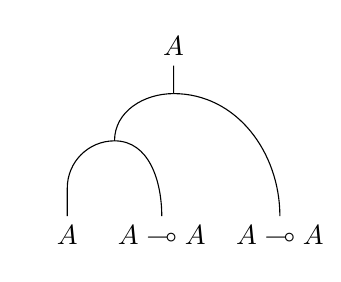
\begin{tikzpicture}[scale=0.3,auto]
\node (topr) at (1.5,2) {$A$};
\coordinate (q) at (-3,-4);
\coordinate (o) at (1.5,0);
\node (delta) at (6,-6) {$A \multimap A$};
\node (gamma) at (-3, -6) {$A$};
\node (ab) at (1,-6) {$A \multimap A$};
\draw[out=90,in=0] (delta) to (o);
\draw (o) to (topr);
\draw[out=90,in=180] (-1,-2) to (o);
\draw[out=90,in=270] (gamma) to (q);
\draw[out=90,in=180] (q) to (-1,-2);
\draw[out=90,in=0] (ab) to (-1,-2);
\end{tikzpicture}
&
$a \otimes \alpha \otimes \beta \mapsto \beta( \alpha(a) )$
\end{tabular}
\end{center}

\begin{center}
% Church numeral 2 layer 3
\begin{tabular}{ >{\centering}m{6cm} >{\centering}m{5cm} >{\centering}m{4cm}}
\AxiomC{}
\UnaryInfC{$A \vdash A$}
\AxiomC{}
\UnaryInfC{$A \vdash A$}
\AxiomC{}
\UnaryInfC{$A \vdash A$}
\RightLabel{\scriptsize$\multimap L$}
\BinaryInfC{$A, A \multimap A \vdash A$}
\RightLabel{\scriptsize$\multimap L$}
\BinaryInfC{$A, A \multimap A, A \multimap A \vdash A$}
\RightLabel{\scriptsize$\multimap R$}
\UnaryInfC{$A \multimap A, A \multimap A \vdash A \multimap A$}
\DisplayProof
&
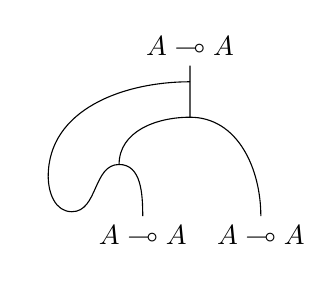
\begin{tikzpicture}[scale=0.3,auto]
\coordinate (o) at (2,0);
\node (top) at ($ (o) + (0,3) $) {$A \multimap A$}; % coordinates are relative to (o)

\coordinate (left_meet) at ($ (o) - (3, 2) $);
\draw[out=90,in=180] (left_meet) to (o);

% Coproduct and derelictions
\node (R) at ($ (o) + (3,-5) $) {$A \multimap A$};
\node (L) at ($ (o) + (-2,-5) $) {$A \multimap A$};
\coordinate (delta) at ($ (o) - (0,5) $);
\draw[out=90,in=0] (R) to (o);

% The A line curl from bottom to top
\coordinate (left_curve) at ($ (o) - (5, 4) $);
\coordinate (left_curve_mid) at ($ (o) - (6,2.5) $);
\coordinate (first_meeting_top) at ($ (o) + (0,1.5) $);
\draw[out=90,in=0] (L) to (left_meet);
\draw[out=0,in=180] (left_curve) to (left_meet);
\draw (o) to (first_meeting_top);
\draw[out=180,in=270] (left_curve) to (left_curve_mid);
\draw[out=90,in=180] (left_curve_mid) to (first_meeting_top);

\draw (first_meeting_top) to (top);
\end{tikzpicture}
&
$\alpha \otimes \beta \mapsto \beta \circ \alpha$
\end{tabular}
\end{center}

\begin{center}
% TIKZ Church numeral 2 layer 4
\begin{tabular}{ >{\centering}m{6cm} >{\centering}m{6cm} >{\centering}m{1cm}}
\AxiomC{}
\UnaryInfC{$A \vdash A$}
\AxiomC{}
\UnaryInfC{$A \vdash A$}
\AxiomC{}
\UnaryInfC{$A \vdash A$}
\RightLabel{\scriptsize$\multimap L$}
\BinaryInfC{$A, A \multimap A \vdash A$}
\RightLabel{\scriptsize$\multimap L$}
\BinaryInfC{$A, A \multimap A, A \multimap A \vdash A$}
\RightLabel{\scriptsize$\multimap R$}
\UnaryInfC{$A \multimap A, A \multimap A \vdash A \multimap A$}
\RightLabel{\scriptsize der}
\UnaryInfC{$!( A \multimap A ), A \multimap A \vdash A \multimap A$}
\RightLabel{\scriptsize der}
\UnaryInfC{$!( A \multimap A ), !(A \multimap A) \vdash A \multimap A$}
\DisplayProof
&
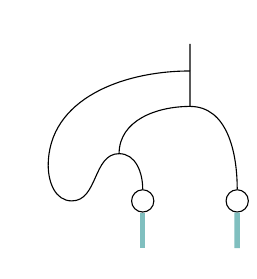
\begin{tikzpicture}[scale=0.3,auto,inner sep=1mm]
\coordinate (o) at (2,0);
\node (top) at ($ (o) + (0,3) $) {}; % coordinates are relative to (o)

\coordinate (left_meet) at ($ (o) - (3, 2) $);
\draw[out=90,in=180] (left_meet) to (o);

% Coproduct and derelictions
\dernode (R) at ($ (o) + (2,-4) $) {};
\dernode (L) at ($ (o) + (-2,-4) $) {};
\coordinate (delta) at ($ (o) - (0,5) $);
\draw[out=90,in=0] (R) to (o);
\drawbang (R) to ($ (R) - (0,2) $);
\drawbang (L) to ($ (L) - (0,2) $);

% The A line curl from bottom to top
\coordinate (left_curve) at ($ (o) - (5, 4) $);
\coordinate (left_curve_mid) at ($ (o) - (6,2.5) $);
\coordinate (first_meeting_top) at ($ (o) + (0,1.5) $);
\draw[out=90,in=0] (L) to (left_meet);
\draw[out=0,in=180] (left_curve) to (left_meet);
\draw (o) to (first_meeting_top);
\draw[out=180,in=270] (left_curve) to (left_curve_mid);
\draw[out=90,in=180] (left_curve_mid) to (first_meeting_top);

\draw (first_meeting_top) to (top);
\end{tikzpicture}
&

\tagarray{\label{2_prime_pre}}

\end{tabular}
\end{center}
The map ${!} \End_k(V) \otimes {!} \End_k(V) \lto \End_k(V)$ in \eqref{2_prime_pre} is zero on $\ket{\nu_1,\ldots,\nu_s}_\alpha \otimes \ket{\mu_1,\ldots,\mu_t}_\beta$ for $\alpha,\beta \in \End_k(V)$ unless $s,t \le 1$, and in those cases it is given by
\begin{align*}
\vacu_\alpha \otimes \vacu_\beta &\longmapsto \beta \circ \alpha\\
\ket{\nu}_\alpha \otimes \vacu_\beta &\longmapsto \beta \circ \nu\\
\vacu_\alpha \otimes \ket{\mu}_\beta &\longmapsto \mu \circ \alpha\\
\ket{\nu}_\alpha \otimes \ket{\mu}_\beta &\longmapsto \mu \circ \nu\,.
\end{align*}
The next deduction rule in $\church{2}_A$ is a contraction:
\begin{center}
% TIKZ Church numeral 2 layer 4
\begin{tabular}{ >{\centering}m{6cm} >{\centering}m{6cm} >{\centering}m{1cm}}
\AxiomC{}
\UnaryInfC{$A \vdash A$}
\AxiomC{}
\UnaryInfC{$A \vdash A$}
\AxiomC{}
\UnaryInfC{$A \vdash A$}
\RightLabel{\scriptsize$\multimap L$}
\BinaryInfC{$A, A \multimap A \vdash A$}
\RightLabel{\scriptsize$\multimap L$}
\BinaryInfC{$A, A \multimap A, A \multimap A \vdash A$}
\RightLabel{\scriptsize$\multimap R$}
\UnaryInfC{$A \multimap A, A \multimap A \vdash A \multimap A$}
\RightLabel{\scriptsize der}
\UnaryInfC{$!( A \multimap A ), A \multimap A \vdash A \multimap A$}
\RightLabel{\scriptsize der}
\UnaryInfC{$!( A \multimap A ), !(A \multimap A) \vdash A \multimap A$}
\RightLabel{\scriptsize ctr}
\UnaryInfC{$!( A \multimap A ) \vdash A \multimap A$}
\DisplayProof
&
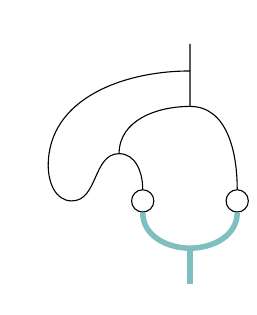
\begin{tikzpicture}[scale=0.3,auto,inner sep=1mm]
\coordinate (o) at (2,0);
\node (top) at ($ (o) + (0,3) $) {}; % coordinates are relative to (o)

\coordinate (left_meet) at ($ (o) - (3, 2) $);
\draw[out=90,in=180] (left_meet) to (o);

% Coproduct and derelictions
\dernode (R) at ($ (o) + (2,-4) $) {};
\dernode (L) at ($ (o) + (-2,-4) $) {};
\coordinate (delta) at ($ (o) - (0,6) $);
\draw[out=90,in=0] (R) to (o);
\drawbang[out=270,in=0] (R) to (delta);
\drawbang[out=270,in=180] (L) to (delta);
\drawbang (delta) to ($ (delta) - (0,1.5) $);

% The A line curl from bottom to top
\coordinate (left_curve) at ($ (o) - (5, 4) $);
\coordinate (left_curve_mid) at ($ (o) - (6,2.5) $);
\coordinate (first_meeting_top) at ($ (o) + (0,1.5) $);
\draw[out=90,in=0] (L) to (left_meet);
\draw[out=0,in=180] (left_curve) to (left_meet);
\draw (o) to (first_meeting_top);
\draw[out=180,in=270] (left_curve) to (left_curve_mid);
\draw[out=90,in=180] (left_curve_mid) to (first_meeting_top);

\draw (first_meeting_top) to (top);
\end{tikzpicture}

&

\tagarray{\label{2_prime}}
\end{tabular}
\end{center}
Let $\phi = \den{\church{2}_A}$ be the linear map ${!} \End_k(V) \lto \End_k(V)$ denoted by this string diagram. Note that this denotation is precisely the composite \eqref{eq:2_as_comp} displayed in Example \ref{example:2_denotation_preview}. We can compute for example the image of $\ket{\nu}_\alpha$ under $\phi$ as follows:
\begin{gather*}
\ket{\nu}_\alpha \longmapsto \ket{\nu}_\alpha \otimes \vacu_\alpha + \vacu_\alpha \otimes \ket{\nu}_\alpha \longmapsto \alpha \circ \nu + \nu \circ \alpha = \{ \nu, \alpha \}\,.
\end{gather*}
This formula is perhaps not surprising as it is the tangent map of the squaring function, see Appendix \ref{section:example_lifting}. Similarly we compute that
\begin{equation}\label{eq:church_2_den}
\phi \vacu_\alpha = \alpha^2, \qquad \phi \ket{\nu}_\alpha = \{ \nu, \alpha \}\,, \qquad \phi \ket{\nu\mu}_\alpha = \{ \nu, \mu \}\,.
\end{equation}
The final step in the proof of $\church{2}_A$ consists of moving the ${!}(A \multimap A)$ to the right side of the turnstile, which yields the final diagram:
% TIKZ ----- Church numeral 2
\begin{equation}\label{church_2_diagram}
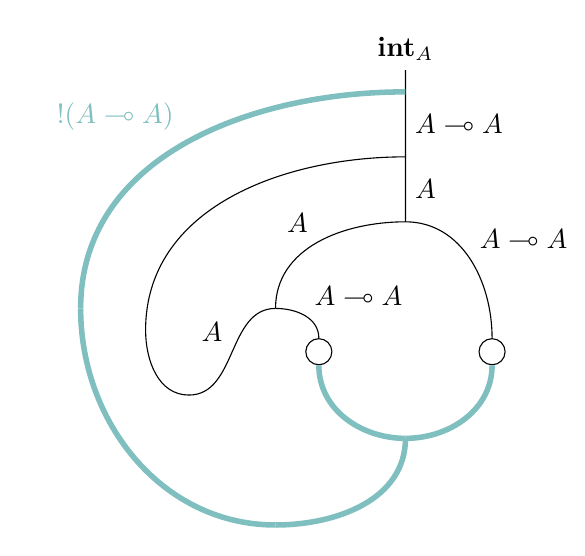
\begin{tikzpicture}[scale=0.55,auto,baseline=(current  bounding  box.center)]
\coordinate (o) at (2,0);
\node (top) at ($ (o) + (0,4) $) {$\inta_A$}; % coordinates are relative to (o)

\coordinate (left_meet) at ($ (o) - (3, 2) $);
\draw[out=90,in=180] (left_meet) to node {$A$} (o);

% Coproduct and derelictions
\dernode (R) at ($ (o) + (2,-3) $) {};
\dernode (L) at ($ (o) + (-2,-3) $) {};
\coordinate (delta) at ($ (o) - (0,5) $);
\draw[out=90,in=0] (R) to node [swap] {$A \multimap A$} (o);
\drawbang[out=0,in=270] (delta) to (R);
\drawbang[out=180,in=270] (delta) to (L);

% The A line curl from bottom to top
\coordinate (left_curve) at ($ (o) - (5, 4) $);
\coordinate (left_curve_mid) at ($ (o) - (6,2.5) $);
\coordinate (first_meeting_top) at ($ (o) + (0,1.5) $);
\draw[out=90,in=0] (L) to node [swap] {$A \multimap A$} (left_meet);
\draw[out=0,in=180] (left_curve) to node {$A$} (left_meet);
\draw (o) to node [swap] {$A$} (first_meeting_top);
\draw[out=180,in=270] (left_curve) to (left_curve_mid);
\draw[out=90,in=180] (left_curve_mid) to (first_meeting_top);

\coordinate (second_meeting_top) at ($ (first_meeting_top) + (0,1.5) $);
\draw (first_meeting_top) to node [swap] {$A \multimap A$} (second_meeting_top);
\draw (second_meeting_top) to (top);

\coordinate (curve_bottom) at ($ (left_meet) - (0,5) $);
\coordinate (curve_left) at ($ (o) - (7.5, 2) $);
\drawbang[out=0,in=270] (curve_bottom) to (delta);
\drawbang[out=180,in=270] (curve_bottom) to (curve_left);
\drawbang[out=90,in=180] (curve_left) to node {$!(A \multimap A)$} (second_meeting_top);
\end{tikzpicture}
\end{equation}
% End Church numeral 2
The denotation of this diagram is the same morphism $\phi$. The reader might like to compare this style of diagram for $\church{2}_A$ to the corresponding proof-net in \cite[\S 5.3.2]{girard_llogic}. 
\end{example}

In Example \ref{example:2_denotation_preview} we sketched how to recover the function $\alpha \mapsto \alpha^2$ from the denotation of the Church numeral $\church{2}_A$, but now we can put this on a firmer footing. There is \emph{a priori} no linear map $\den{B} \lto \den{C}$ associated to $\pi$ but there is a function $\den{\pi}_{nl}$ ($nl$ standing for \emph{nonlinear}) defined on $P \in \den{B}$ by lifting to $! \den{B}$ and then applying $\den{\pi}$:
\begin{equation}\label{eq:lifting_vacua}
\xymatrix@C+2pc{
k \ar[r]^-{P} \ar@{.>}[dr]_-{\vacu_P} & \den{B} & \den{C}\\
& ! \den{B} \ar[u]_-{d} \ar[ur]_-{\den{\pi}}
}\,.
\end{equation}
%We saw an example of this pattern in Example \ref{example:church_2}.
That is,

\begin{definition}\label{defn:nonlinear_denotation}
The function $\den{\pi}_{nl}: \den{B} \lto \den{C}$ is defined by $\den{\pi}_{nl}(P) = \den{\pi} \vacu_P$.
\end{definition}

The discussion above shows that, with $V = \den{A}$,

\begin{lemma}\label{lemma:nonlinear_recover} $\den{\church{2}_A}_{nl}: \End_k(V) \lto \End_k(V)$ is the map $\alpha \mapsto \alpha^2$.
\end{lemma}

This completes our explanation of how to represent the Church numeral $\church{2}_A$ as a linear map. From this presentation we see clearly that the non-linearity of the map $\alpha \mapsto \alpha^2$ is concentrated in the promotion step \eqref{eq:lifting_vacua} where the input vector $\alpha$ is turned into a vacuum $\vacu_\alpha \in {!} \End_k(V)$. The promotion step is non-linear since $\vacu_\alpha + \vacu_\beta$ is not a morphism of coalgebras and thus cannot be equal to $\vacu_{\alpha + \beta}$. After this step, the duplication, dereliction and composition shown in \eqref{eq:2_deals_with_0} are all linear. %Finally, when $k = \mathbb{C}$ it is interesting to compare $\den{2}_{nl}$ with the map $\alpha \mapsto \alpha^2$ of smooth manifolds $\End_k(V)$, see Appendix \ref{section:example_lifting}.

%(see the discussion of tangents in Appendix \ref{section:example_lifting}) 

% Let $\church{2}_A'$ denote the proof of ${!}(A \multimap A) \vdash A \multimap A$ in \eqref{2_prime}. As discussed in Example \ref{example:denotation_2}, we may confuse the denotation of $\church{2}_A$ and $\church{2}_A'$. 
\begin{example}\label{example:2_promotion} Applied to $\church{2}_A$ the promotion rule generates a new proof
\begin{prooftree}
\AxiomC{$\church{2}_A$}
\noLine\UnaryInfC{$\vdots$}
\def\extraVskip{5pt}
\noLine\UnaryInfC{$!(A \multimap A) \vdash A \multimap A$}
\def\extraVskip{2pt}
\RightLabel{\scriptsize prom}
\UnaryInfC{$!( A \multimap A) \vdash {!}(A \multimap A)$}
\end{prooftree}
which we denote $\operatorname{prom}( \church{2}_A )$. By definition the denotation $\Phi := \den{ \operatorname{prom}( \church{2}_A ) }$ of this proof is the unique morphism of coalgebras
\[
\Phi: {!} \End_k(V) \lto {!} \End_k(V)
\]
with the property that $d \circ \Phi = \phi$, where $\phi = \den{\church{2}_A}$ is as in \eqref{eq:2_as_comp}. From \eqref{eq:church_2_den} and Theorem \ref{theorem:describe_lifting} we compute that, for example
\begin{align*}
\Phi \vacu_\alpha &= \vacu_{\alpha^2}\,,\\
\Phi \ket{\nu}_\alpha &= \{ \nu, \alpha \} \cdot \vacu_{\alpha^2},\\
\Phi \ket{\nu \mu}_\alpha &= \big( \{ \nu, \mu \} + \{ \nu, \alpha \} \otimes \{ \mu, \alpha \} \big) \cdot \vacu_{\alpha^2}\,,\\
\Phi \ket{\nu \mu \theta}_\alpha &= \big( \{ \nu, \mu \} \otimes \{ \theta, \alpha \} + \{ \theta, \mu \} \otimes \{ \nu, \alpha \} + \{ \nu, \theta \} \otimes \{ \mu, \alpha \}\\
&+ \{ \nu, \alpha \} \otimes \{ \mu, \alpha \} \otimes \{ \theta, \alpha \} \big) \cdot \vacu_{\alpha^2}\,.
\end{align*}
Note that the commutators, e.g. $\{ \nu, \alpha \}$ are defined using the product internal to $\End_k(V)$, whereas inside the bracket in the last two lines, the terms $\{ \nu, \alpha \}$ and $\{ \mu, \alpha \}$ are multiplied in the algebra $\Sym( \End_k(V) )$ before being made to act on the vacuum.
\end{example}

%The approach we have chosen has the advantage of being universal in a certain sense: given another categorical semantics, say in a closed symmetric monoidal category $\cat{T}$ with comonad $Q$ modelling the exponential, if there is a strong monoidal functor $F: \cat{T} \lto \cat{V}$ (e.g. the objects of $\cat{T}$ are vector spaces with additional structure) then for any object $V \in \cat{T}$ the morphism $QV \lto V$ becomes a map $FQV \lto FV$, and since $FQV$ is a coalgebra, this factors as
%\[
%\xymatrix@C+1.5pc@R+1.5pc{
%FQV \ar[r]\ar[dr] & FV\\
%& {!}FV \ar[u]_-{d}
%}
%\]
%In this way it is possible to relate semantics such as Ehrhard's finiteness spaces \cite{ehrhard} to the ``universal'' semantics defined above.
\begin{remark}\label{remark_otherpromotion} As we have already mentioned, there are numerous semantics of linear logic defined using topological vector spaces. The reader curious about how these vector space semantics are related to the ``relational'' style of semantics such as coherence spaces should consult Ehrhard's paper on finiteness spaces \cite{ehrhard}.

One can generate simple variants on the vector space semantics by looking at comonads on the category $\cat{V}$ defined by truncations on the coalgebras ${!} V$. For example, given a vector space $V$, let ${!}_0 V$ denote the subspace of ${!} V$ generated by the vacua $\vacu_P$. This is the free space on the underlying \emph{set} of $V$, and it is a subcoalgebra of ${!} V$ given as a coproduct of trivial coalgebras. It is easy to see that this defines an appropriate comonad and gives rise to a semantics of linear logic \cite[\S 4.3]{valiron}. However the semantics defined using ${!} V$ is more interesting, because universality allows us to mix in arbitrary coalgebras $C$. In Appendix \ref{section:example_lifting} we examine the simplest example where $C$ is the dual of the algebra $k[t]/t^2$ and relate this to tangent vectors.
\end{remark}

\section{Cut-elimination}\label{section:cut_elim}
%The formulas and proofs, to borrow an analogy from \cite[\S III]{girard_towards}, play within linear logic a role analogous to that of statics within classical mechanics. 

The dynamical part of linear logic is a rewrite rule on proofs called \emph{cut-elimination}, which defines the way that proofs interact and is the analogue in linear logic of $\beta$-reduction in the $\lambda$-calculus. Collectively these interactions give the connectives their meaning. The full set of rewrite rules is given in \cite[Section 3]{mellies} and in the alternative language of proof-nets in \cite[\S 4]{girard_llogic}, \cite[p.18]{pagani}. We will not reproduce the full list here because it takes up several pages and there are some subtle cases. That being said, we do not wish to leave the reader with the impression that these rules are mysterious: the key rules have a clear conceptual content, which we elucidate in this section by presenting a worked example involving our favourite proof $\church{2}_A$ and the string diagram transformations associated to the rewrites.

\begin{definition} Let $\Gamma \vdash A$ be a sequent of linear logic and $\cat{P}$ the set of proofs. There is a binary relation $\rightsquigarrow$ on $\cat{P}$ defined by saying that $\pi \rightsquigarrow \rho$ if $\rho$ is an immediate reduction of $\pi$ by one of the rewrite rules listed in \cite[Section 3]{mellies}. These rewrite rules are sometimes referred to as \emph{cut-elimination transformations}.

We write $=_{cut}$ for the smallest reflexive, transitive and symmetric relation on $\cat{P}$ containing $\rightsquigarrow$ and call this \emph{equivalence under cut-elimination}.
\end{definition}

%The rewrite rules listed in \cite[Section 3]{mellies}  %Conceptually, if $\pi \rightsquigarrow \rho$ then $\pi$ and $\rho$ contain the same logical content, but this content is expressed more explicitly in $\rho$. 

\begin{example}
In the context of Example \ref{example:cutagainst2} there is a sequence of transformations
\[
\church{2}_A \l \operatorname{prom}( \pi ) = \pi_0 \rightsquigarrow \pi_1 \rightsquigarrow \cdots \rightsquigarrow \pi \l \pi
\]
which begins with the rewrites \cite[\S 3.9.3]{mellies} and \cite[\S 3.9.1]{mellies}.
\end{example}

\begin{example}\label{example:cut_elim_examples} The cut-elimination transformation \cite[\S 3.8.2]{mellies} tells us that
\begin{center}
\begin{tabular}{ >{\centering}m{7cm} >{\centering}m{4cm} >{\centering}m{3cm}}
\AxiomC{$\pi_2$}
\noLine\UnaryInfC{$\vdots$}
\def\extraVskip{5pt}
\noLine\UnaryInfC{$A \vdash B$}
\def\extraVskip{2pt}
\RightLabel{\scriptsize $\multimap R$}
\UnaryInfC{$\vdash A \multimap B$}
\AxiomC{$\pi_1$}
\noLine\UnaryInfC{$\vdots$}
\def\extraVskip{5pt}
\noLine\UnaryInfC{$\Gamma \vdash A$}
\def\extraVskip{2pt}
\AxiomC{$\pi_3$}
\noLine\UnaryInfC{$\vdots$}
\def\extraVskip{5pt}
\noLine\UnaryInfC{$B \vdash C$}
\def\extraVskip{2pt}
\RightLabel{\scriptsize $\multimap L$}
\BinaryInfC{$\Gamma, A \multimap B \vdash C$}
\RightLabel{\scriptsize cut}
\BinaryInfC{$\Gamma \vdash C$}
\DisplayProof
&
\begin{tikzpicture}[scale=0.35,auto]
\node (top) at (0,5) {$C$};
\mapnode (mid_top) at (0,2) {};
\node [above] at (mid_top.east) {$\;\;\;\;\;\;\den{\pi_3}$};
\node (bottoml) at (-3,-5) {$\Gamma$};
\mapnode (pi1) at (-3,-3) {};
\node [above] at (pi1.east) {$\;\;\;\;\;\;\;\;\;\den{\pi_1}$};
\coordinate (o) at (0,0);
\draw (o) -- (mid_top);
\draw (mid_top) -- (top);
\draw (bottoml) -- (pi1);
\draw[out=90,in=180] (pi1) to (o);
\mapnode (other) at (3,-3) {};
\coordinate (other_up) at (3,-2) {};
\node [right] at (other.east) {$\den{\pi_2}$};
\draw[out=90,in=0] (other_up) to (o);
\draw (other) to (other_up);
\coordinate (turn) at ($ (other) - (1.5,2) $);
\coordinate (upper_turn) at ($ (turn) + (-1,1) $);
\draw[out=270,in=0] (other) to (turn);
\draw[out=180,in=270] (turn) to (upper_turn);
\draw[out=90,in=180] (upper_turn) to (other_up);
\end{tikzpicture}
&
\tagarray{\label{eq:cutelim3}}
\end{tabular}
\end{center}
may be transformed to
\begin{center}
\begin{tabular}{ >{\centering}m{8cm} >{\centering}m{3cm} >{\centering}m{3cm}}
\AxiomC{$\pi_1$}
\noLine\UnaryInfC{$\vdots$}
\def\extraVskip{5pt}
\noLine\UnaryInfC{$\Gamma \vdash A$}
\def\extraVskip{2pt}
\AxiomC{$\pi_2$}
\noLine\UnaryInfC{$\vdots$}
\def\extraVskip{5pt}
\noLine\UnaryInfC{$A \vdash B$}
\def\extraVskip{2pt}
\RightLabel{\scriptsize cut}
\BinaryInfC{$\Gamma \vdash B$}
\AxiomC{$\pi_3$}
\noLine\UnaryInfC{$\vdots$}
\def\extraVskip{5pt}
\noLine\UnaryInfC{$B \vdash C$}
\def\extraVskip{2pt}
\RightLabel{\scriptsize cut}
\BinaryInfC{$\Gamma \vdash C$}
\DisplayProof
&
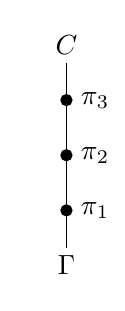
\begin{tikzpicture}[scale=0.35,auto,inner sep=1mm]
\node (top) at (0,5) {$C$};
\mapnode (pi3) at (0,3) {};
\node [right] at (pi3.east) {$\den{\pi_3}$};
\mapnode (pi2) at (0,1) {};
\node [right] at (pi2.east) {$\den{\pi_2}$};
\mapnode (pi1) at (0,-1) {};
\node [right] at (pi1.east) {$\den{\pi_1}$};
\node (bottom) at (0,-3) {$\Gamma$};
\draw (bottom) -- (pi1);
\draw (pi1) -- (pi2);
\draw (pi2) -- (pi3);
\draw (pi3) -- (top);
\end{tikzpicture}
&
\tagarray{\label{eq:cutelim4}}
\end{tabular}
\end{center}
Observe how this cut-elimination transformation encodes the meaning of the left introduction rule $\multimap L$, in the sense that it takes a proof $\pi_1$ of $\Gamma \vdash A$ and a proof $\pi_3$ of $B \vdash C$ and says: if you give me a proof of $A \vdash B$ I know how to sandwich it between $\pi_1$ and $\pi_3$.
\end{example}

\begin{example}\label{example:cut_elim_examples2} The cut-elimination transformation \cite[\S 3.11.10]{mellies} tells us that
\begin{center}
\begin{tabular}{ >{\centering}m{7cm} >{\centering}m{4cm} >{\centering}m{3cm}}
\AxiomC{$\pi_1$}
\noLine\UnaryInfC{$\vdots$}
\def\extraVskip{5pt}
\noLine\UnaryInfC{$\Gamma \vdash A$}
\def\extraVskip{2pt}
\AxiomC{$\pi_2$}
\noLine\UnaryInfC{$\vdots$}
\def\extraVskip{5pt}
\noLine\UnaryInfC{$B, A \vdash C$}
\def\extraVskip{2pt}
\RightLabel{\scriptsize $\multimap R$}
\UnaryInfC{$A \vdash B \multimap C$}
\RightLabel{\scriptsize cut}
\BinaryInfC{$\Gamma \vdash B \multimap C$}
\DisplayProof
&
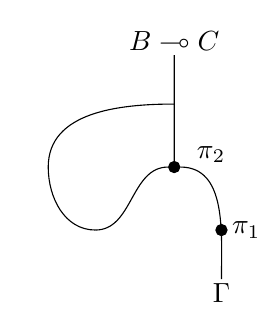
\begin{tikzpicture}[inner sep = 0.5mm, scale=0.4,auto]
\node (topr) at (1,4) {$B \multimap C$};
\node[circle,draw=black,fill=black] (o) at (1,0) {};
\node [above] at (o.east) {$\;\;\;\;\;\;\;\;\den{\pi_2}$};
\node[circle,draw=black,fill=black] (other) at (2.5,-2) {};
\node [right] at (other.east) {$\den{\pi_1}$};
\node (gamma) at (2.5,-4) {$\Gamma$};
\draw[out=90,in=0] (gamma) to (o);
\draw[out=0,in=180] (-1.5,-2) to (o);
\draw[out=180,in=270] (-1.5,-2) to (-3,0);
\draw[out=90,in=180] (-3,0) to (1,2);
\draw (o) to (1,2);
\draw (1,2) to (topr);
\end{tikzpicture}
&
\tagarray{\label{eq:cutelim1}}
\end{tabular}
\end{center}
is transformed to the proof
\begin{center}
\begin{tabular}{ >{\centering}m{7cm} >{\centering}m{4cm} >{\centering}m{3cm}}
\AxiomC{$\pi_1$}
\noLine\UnaryInfC{$\vdots$}
\def\extraVskip{5pt}
\noLine\UnaryInfC{$\Gamma \vdash A$}
\def\extraVskip{2pt}
\AxiomC{$\pi_2$}
\noLine\UnaryInfC{$\vdots$}
\def\extraVskip{5pt}
\noLine\UnaryInfC{$B, A \vdash C$}
\def\extraVskip{2pt}
\RightLabel{\scriptsize cut}
\BinaryInfC{$B, \Gamma \vdash C$}
\RightLabel{\scriptsize $\multimap R$}
\UnaryInfC{$\Gamma \vdash B \multimap C$}
\DisplayProof
&
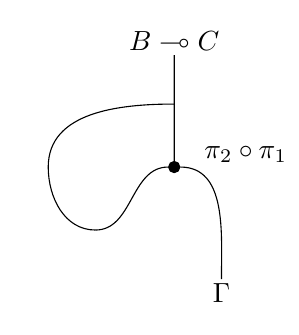
\begin{tikzpicture}[inner sep = 0.5mm, scale=0.4,auto]
\node (topr) at (1,4) {$B \multimap C$};
\node[circle,draw=black,fill=black] (o) at (1,0) {};
\node [above] at (o.east) {$\;\;\;\;\;\;\;\;\;\;\;\;\;\;\;\;\;\den{\pi_2} \circ \den{\pi_1}$};
\node (gamma) at (2.5,-4) {$\Gamma$};
\draw[out=90,in=0] (gamma) to (o);
\draw[out=0,in=180] (-1.5,-2) to (o);
\draw[out=180,in=270] (-1.5,-2) to (-3,0);
\draw[out=90,in=180] (-3,0) to (1,2);
\draw (o) to (1,2);
\draw (1,2) to (topr);
\end{tikzpicture}
&
\tagarray{\label{eq:cutelim2}}
\end{tabular}
\end{center}
and thus the two corresponding diagrams are equal. In this case, the equality generated by cut-elimination expresses the fact that the Hom-tensor adjunction is natural.
\end{example}

\begin{example}\label{example:cut_elim_examples3} The cut-elimination transformation \cite[\S 3.6.1]{mellies} tells us that
\begin{center}
\AxiomC{} 
\UnaryInfC{$A \vdash A$}
\AxiomC{$\pi$}
\noLine\UnaryInfC{$\vdots$}
\def\extraVskip{5pt}
\noLine\UnaryInfC{$A \vdash B$}
\RightLabel{\scriptsize cut}
\BinaryInfC{$A \vdash B$}
\DisplayProof
\end{center}
may be transformed to the proof $\pi$. Thus the axiom rule acts as an identity for cut.
\end{example}

The analogue in linear logic of a normal form in $\lambda$-calculus is

\begin{definition} A proof is \emph{cut-free} if it contains no occurrences of the cut rule.
\end{definition}

The main theorem is that the relation $\rightsquigarrow$ is \emph{weakly normalising}, which means:

\begin{theorem}[Cut-elimination] For each proof $\pi$ in linear logic there is a sequence
\begin{equation}\label{eq:proof_pi}
\pi = \pi_0 \rightsquigarrow \pi_1 \rightsquigarrow \cdots \rightsquigarrow \pi_n = \widetilde{\pi}
\end{equation}
where $\widetilde{\pi}$ is cut-free, and $n$ depends on $\pi$.
\end{theorem}
\begin{proof}
The original proof by Girard is given in the language of proof-nets \cite{girard_llogic}. For a proof in the language of sequent calculus see for example \cite[Appendix B]{brauner}. The argument follows Gentzen's proof for cut-elimination in classical logic; see \cite{gentzen} and \cite[Chapter 13]{girard_prooftypes}. 
\end{proof}

This is the analogue of Gentzen's \emph{Hauptsatz} for ordinary logic, which was mentioned in the introduction. At a high level, the sequence of rewrites \eqref{eq:proof_pi} eliminates the implicitness present in the original proof until the fully explicit, cut-free proof $\widetilde{\pi}$ is left. %In practice there are various kinds of cut-elimination transformations, for example:
%\begin{itemize}
%\item those like \eqref{eq:cutelim1} $\rightsquigarrow$ \eqref{eq:cutelim2} in Example \ref{example:cut_elim_examples} which commute cuts past other deduction rules or otherwise rearrange the content of the proof.
%\item those like \eqref{eq:cutelim3} $\rightsquigarrow$ \eqref{eq:cutelim4} in Example \ref{example:cut_elim_examples2} which replace a cut on a complex formula $A \multimap B$ by cuts on simpler formulae $A,B$. 
%\item those like the transformation in Example \ref{example:cut_elim_examples3} which actually erase part of the proof.
% With some abuse of language (to be discussed in a moment) we will refer below to $\pi_n$ as the \emph{cut-free normalisation} of $\pi$.
%\end{itemize}

\begin{remark} It is possible that multiple rewrite rules apply to a given proof, so that there is more than one sequence \eqref{eq:proof_pi} with $\pi$ as its starting point. This raises the natural question: does \emph{every} sequence of rewrites starting from $\pi$ terminate with a cut-free proof? This property of a rewrite rule is called \emph{strong normalisation}. We could also ask whether it is the case that whenever a proof $\pi$ reduces to $\pi'$ as well as to $\pi''$, there exists a proof $\pi'''$ to which both of the proofs $\pi'$ and $\pi''$ reduce; this is called \emph{confluence} or the \emph{Church-Rosser property}. If a rewrite rule satisfies both strong normalisation and confluence then beginning with a proof $\pi$ we can apply arbitrarily chosen reductions and be assured that eventually this process terminates, and that the result is independent of all choices: that is, the result is a \emph{normal form} of $\pi$.

Unfortunately in its sequent calculus presentation linear logic does \emph{not} satisfy confluence and in particular it is not true that each cut-elimination equivalence class contains a unique cut-free proof \cite[\S 1.3.1]{girard_prooftypes}. However to some extent this is a ``mere'' technical problem, and is usually taken as evidence that the right presentation of linear logic is not via the (overly bureaucratic) sequent calculus but through \emph{proof-nets}. In Girard's original paper \cite[III.3]{girard_llogic} it is proven that cut-elimination for proof-nets satisfies strong normalisation in the current setting of first-order linear logic; regarding second-order linear logic and confluence the story is surprisingly intricate, see \cite{pagani}. Note also that the Natural Deduction presentation of linear logic is very close to the sequent calculus and satisfies both strong normalisation and confluence; see \cite{benton_strong} and \cite[\S 2.2]{brauner}.
\end{remark}

\subsection{An extended example}

To demonstrate cut-elimination in a nontrivial example, let us prove that $2 \times 2 = 4$.

\begin{definition}\label{definition:mult_m} Let $m \ge 0$ be an integer and $A$ a formula. We define $\prf{\mathrm{mult}}_A(m, -)$ to be the proof (writing $E = A \multimap A$)
\begin{equation}\label{cut_mult_2_0}
% TIKZ Church numeral 2 layer 4
\begin{mathprooftree}
\AxiomC{$\church{m}_A$}
\noLine\UnaryInfC{$\vdots$}
\def\extraVskip{5pt}
\noLine\UnaryInfC{${!}E \vdash E$}
\def\extraVskip{2pt}
\RightLabel{\scriptsize prom}
\UnaryInfC{${!}E \vdash {!}E$}
\AxiomC{}
\UnaryInfC{$E \vdash E$}
\RightLabel{\scriptsize$\multimap L$}
\BinaryInfC{${!} E, \inta_A \vdash E$}
\RightLabel{\scriptsize$\multimap R$}
\UnaryInfC{$\inta_A \vdash \inta_A$}
\end{mathprooftree}
\end{equation}
\end{definition}

This proof represents multiplication by $m$, in the following sense.

\begin{lemma} The proof obtained from $\prf{\mathrm{mult}}_A(m,-)$ by cutting against $\church{n}_A$
\begin{equation}\label{cut_mult_prooftree}
\begin{mathprooftree}
\AxiomC{$\church{n}_A$}
\noLine\UnaryInfC{$\vdots$}
\def\extraVskip{5pt}
\noLine\UnaryInfC{$\vdash \inta_A$}
\def\extraVskip{2pt}
\AxiomC{$\prf{\mathrm{mult}}_A(m,-)$}
\noLine\UnaryInfC{$\vdots$}
\def\extraVskip{5pt}
\noLine\UnaryInfC{$\inta_A \vdash \inta_A$}
\def\extraVskip{2pt}
\RightLabel{\scriptsize cut}
\BinaryInfC{$\vdash \inta_A$}
\end{mathprooftree}
\end{equation}
is equivalent under cut-elimination to $\church{mn}_A$.
\end{lemma}

Rather than give a complete proof of this lemma, we examine the special case where $m = n = 2$. If we denote the proof in \eqref{cut_mult_prooftree} by $\prf{\mathrm{mult}}_A(2,-) \l \church{2}_A$ then its string diagram is
\begin{equation}\label{cut_mult_2}
% TIKZ ---- picture of mult_2
\prf{\mathrm{mult}}_A(2,-) \l \church{2}_A \quad = 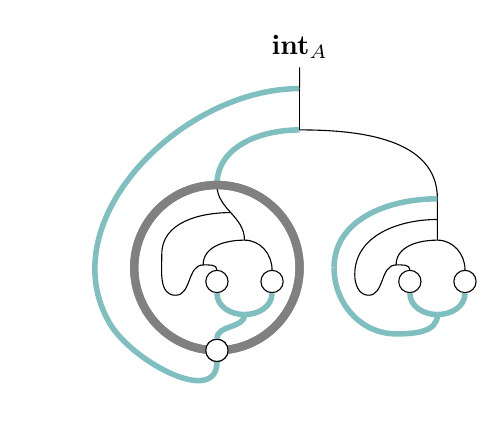
\begin{tikzpicture}[scale=0.35,auto,inner sep=1mm,baseline=(current  bounding  box.center)]
\coordinate (topr) at (0,2);
\coordinate (comp) at (3,4);
\drawbang[out=90,in=180] (topr) to (comp);
\drawprom (0,-1) ellipse (3cm and 3cm);
\dernode (bottomr) at (0,-4) {};

% -------- promoted 2 ---------
% All coordinates are relative to the composition vertex (o), which itself
% has its coordinates derived from topr. This is the only link to the outside namespace.
\coordinate (o) at ($ (topr) + (1,-2) $);
\coordinate (ellipse_center) at ($ (o) - (1,1) $);
\coordinate (elbow) at ($ (o) - (3, 0.5) $);
\coordinate (top_of_circle) at ($ (o) + (-1,2) $);
\draw[out=90,in=270] (o) to (top_of_circle);
\drawprom (ellipse_center) ellipse (3cm and 3cm); % outer boundary
\dernode (bottomr) at ($ (o) - (1,4) $) {};
\dernode (R) at ($ (o) + (1, -1.5) $) {}; % right dereliction
\dernode (L) at ($ (o) - (1,1.5) $) {}; % left dereliction
\coordinate (left_curve) at ($ (o) - (2.5,2) $);
\coordinate (left_meet) at ($ (o) - (1.5, 0.9) $);
\coordinate (delta) at ($ (o) - (0, 2.7) $); % coproduct vertex
\draw[out=90,in=0] (R) to node [swap] {} (o);
\drawbang[out=0,in=270] (delta) to (R);
\drawbang[out=180,in=270] (delta) to (L);
\drawbang[out=90,in=270] (bottomr) to (delta);
\draw[out=90,in=180] (left_meet) to (o);
\draw[out=90,in=0] (L) to (left_meet);
\draw[out=0,in=180] (left_curve) to (left_meet);
\draw[out=180,in=270] (left_curve) to (elbow);
\draw[out=90,in=180] (elbow) to ($ (o)!.5!(top_of_circle) $);
% ------ end promoted 2 ------

% Now for the rest of the diagram
\coordinate (curve) at (-3.9, -3);
\coordinate (meet) at (3,5.5);
\drawbang[out=300,in=270] (curve) to (bottomr);
\drawbang[out=120,in=180] (curve) to (meet);
\node (vtop) at (3,7) {$\inta_A$};
\draw (meet) to (vtop);
\draw (comp) to (meet);

% ----------The Church 2 on the right
\coordinate (2o) at ($ (topr) + (8,-2) $);

\coordinate (2left_meet) at ($ (2o) - (1.5, 0.9) $);
\draw[out=90,in=180] (2left_meet) to (2o);

% Coproduct and derelictions
\dernode (2R) at ($ (2o) + (1,-1.5) $) {};
\dernode (2L) at ($ (2o) + (-1,-1.5) $) {};
\coordinate (2delta) at ($ (2o) - (0,2.7) $);
\draw[out=90,in=0] (2R) to (2o);
\drawbang[out=0,in=270] (2delta) to (2R);
\drawbang[out=180,in=270] (2delta) to (2L);

% The A line curl from bottom to top
\coordinate (2left_curve) at ($ (2o) - (2.5, 2) $);
\coordinate (2left_curve_mid) at ($ (2o) - (3,1.25) $);
\coordinate (2first_meeting_top) at ($ (2o) + (0,0.75) $);
\draw[out=90,in=0] (2L) to (2left_meet);
\draw[out=0,in=180] (2left_curve) to (2left_meet);
\draw[out=180,in=270] (2left_curve) to (2left_curve_mid);

\coordinate (2curve_bottom) at ($ (2left_meet) - (0,2.5) $);
\coordinate (2curve_left) at ($ (2o) - (3.75, 1) $);
\drawbang[out=0,in=270] (2curve_bottom) to (2delta);
\drawbang[out=180,in=270] (2curve_bottom) to (2curve_left);


% the lines from the right 2 to the comp vertex are scaled along the line
\coordinate (2top) at ($ (2o) + (0,1.5) $);
\draw[out=90,in=0] (2top) to (comp);
\draw (2o) to (2top);
\drawbang[out=90,in=180] (2curve_left) to (2top);
\draw[out=90,in=180] (2left_curve_mid) to ($ (2o)!.5!(2top) $);
\end{tikzpicture}
\end{equation}
To prove that the cut-free normalisation of $\prf{\mathrm{mult}}_A(2,-) \l \church{2}_A$ is the Church numeral $\church{4}_A$ we run through the proof transformations generated by the cut-elimination algorithm, each of which yields a new proof with the same denotation. This sequence of proofs represents the following sequence of manipulations of the string diagram:
\begin{itemize}
\item The first reduction \eqref{eq:cutelim1} $\rightsquigarrow$ \eqref{eq:cutelim2} applies naturality of the Hom-tensor adjunction to \eqref{cut_mult_2}. Then we are in the position of \eqref{eq:cutelim3}, with $\pi_2$ a part of $\church{2}_A$ and $\pi_1$ the promoted Church numeral and the reduction \eqref{eq:cutelim3} $\rightsquigarrow$ \eqref{eq:cutelim4} takes the left leg of the diagram and feeds it as an input to the right leg.
\item Next, we use that a promotion box represents a morphism of coalgebras, and thus can be commuted past the coproduct whereby it is duplicated.
\item Then the promotions cancel with the derelictions by the identity \eqref{eq:prom_cancel_der}, ``releasing'' the pair of Church numerals contained in the promotion boxes.
\item Finally, we may apply the general form of \eqref{eq:cutelim3} $\rightsquigarrow$ \eqref{eq:cutelim4}.
\end{itemize}
Each of these steps corresponds to one of the equalities in the following chain of diagrams:
\begin{equation}\label{diagram_mult_2_2}
% TIKZ picture ---- stacked 2 promotions LEFT
\prf{\mathrm{mult}}_A(2,-) \l \church{2}_A \ = \ 
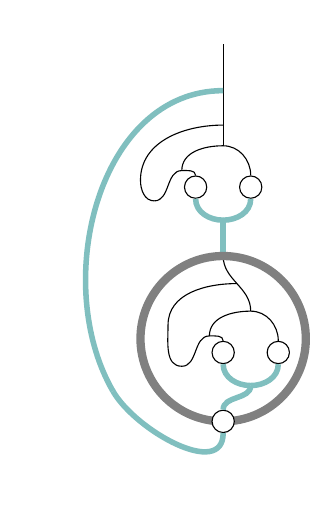
\begin{tikzpicture}[scale=0.35,auto,inner sep=1mm,baseline=(current  bounding  box.center)]
\coordinate (topr) at (0,2); % top of the bottom promoted 2
\coordinate (curve) at (-4, -2.9);
%\coordinate (comp) at (0,4) {};
\node (vtop) at ($ (topr) + (0,8) $) {};
\coordinate (meet) at ($ (vtop) - (0,2) $); % where the curved !( A -o A ) arc meets at the top

\draw (meet) to (vtop);

% ----------The Church 2 on the right
\coordinate (2o) at ($ (topr) + (0,4) $);
\coordinate (2left_meet) at ($ (2o) - (1.5, 0.9) $);
\draw[out=90,in=180] (2left_meet) to (2o);

% Coproduct and derelictions
\dernode (2R) at ($ (2o) + (1,-1.5) $) {};
\dernode (2L) at ($ (2o) + (-1,-1.5) $) {};
\coordinate (2delta) at ($ (2o) - (0,2.7) $);
\draw[out=90,in=0] (2R) to (2o);
\drawbang[out=0,in=270] (2delta) to (2R);
\drawbang[out=180,in=270] (2delta) to (2L);

% The A line curl from bottom to top
\coordinate (2left_curve) at ($ (2o) - (2.5, 2) $);
\coordinate (2left_curve_mid) at ($ (2o) - (3,1.25) $);
\coordinate (2first_meeting_top) at ($ (2o) + (0,0.75) $);
\draw[out=90,in=0] (2L) to (2left_meet);
\draw[out=0,in=180] (2left_curve) to (2left_meet);
\draw[out=180,in=270] (2left_curve) to (2left_curve_mid);
\draw[out=90,in=180] (2left_curve_mid) to (2first_meeting_top);
\draw (2o) to (meet);

%\draw[out=90,in=270] (2join_at_top) to (meet);
\drawbang (topr) to (2delta);

% -------- promoted 2 ---------
% All coordinates are relative to the composition vertex (o), which itself
% has its coordinates derived from topr. This is the only link to the outside namespace.
\coordinate (o) at ($ (topr) + (1,-2) $);
\coordinate (ellipse_center) at ($ (o) - (1,1) $);
\coordinate (elbow) at ($ (o) - (3, 0.5) $);
\coordinate (top_of_circle) at ($ (o) + (-1,2) $);
\draw[out=90,in=270] (o) to (top_of_circle);
\drawprom (ellipse_center) ellipse (3cm and 3cm); % outer boundary
\dernode (bottomr) at ($ (o) - (1,4) $) {};
\dernode (R) at ($ (o) + (1, -1.5) $) {}; % right dereliction
\dernode (L) at ($ (o) - (1,1.5) $) {}; % left dereliction
\coordinate (left_curve) at ($ (o) - (2.5,2) $);
\coordinate (left_meet) at ($ (o) - (1.5, 0.9) $);
\coordinate (delta) at ($ (o) - (0, 2.7) $); % coproduct vertex
\draw[out=90,in=0] (R) to node [swap] {} (o);
\drawbang[out=0,in=270] (delta) to (R);
\drawbang[out=180,in=270] (delta) to (L);
\drawbang[out=90,in=270] (bottomr) to (delta);
\draw[out=90,in=180] (left_meet) to (o);
\draw[out=90,in=0] (L) to (left_meet);
\draw[out=0,in=180] (left_curve) to (left_meet);
\draw[out=180,in=270] (left_curve) to (elbow);
\draw[out=90,in=180] (elbow) to ($ (o)!.5!(top_of_circle) $);
% ------ end promoted 2 ------

% The loop from the bottom of the promoted 2 up to the top
\drawbang[out=300,in=270] (curve) to (bottomr);
\drawbang[out=120,in=180] (curve) to (meet);
\end{tikzpicture}
\quad = \quad
% ---------------------- TIKZ stacked 2's, RIGHT
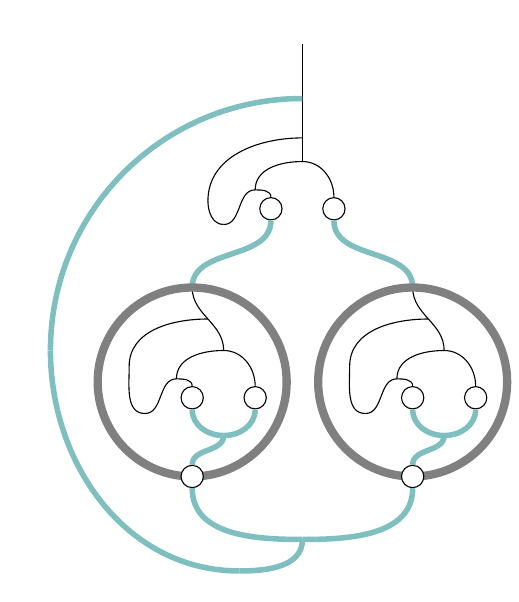
\begin{tikzpicture}[scale=0.4,auto,inner sep=1mm,baseline=(current  bounding  box.center)]
\coordinate (topr) at (0,2); % top of the bottom promoted 2
%\coordinate (comp) at (0,4) {};
\node (vtop) at ($ (topr) + (0,8) $) {};
\coordinate (meet) at ($ (vtop) - (0,2) $); % where the curved !( A -o A ) arc meets at the top

\draw (meet) to (vtop);

% ----------The Church 2 on top
\coordinate (2o) at ($ (topr) + (0,4) $);
\coordinate (2left_meet) at ($ (2o) - (1.5, 0.9) $);
\draw[out=90,in=180] (2left_meet) to (2o);

% Coproduct and derelictions
\dernode (2R) at ($ (2o) + (1,-1.5) $) {};
\dernode (2L) at ($ (2o) + (-1,-1.5) $) {};
\draw[out=90,in=0] (2R) to (2o);

% The A line curl from bottom to top
\coordinate (2left_curve) at ($ (2o) - (2.5, 2) $);
\coordinate (2left_curve_mid) at ($ (2o) - (3,1.25) $);
\coordinate (2first_meeting_top) at ($ (2o) + (0,0.75) $);
\draw[out=90,in=0] (2L) to (2left_meet);
\draw[out=0,in=180] (2left_curve) to (2left_meet);
\draw[out=180,in=270] (2left_curve) to (2left_curve_mid);
\draw[out=90,in=180] (2left_curve_mid) to (2first_meeting_top);
\draw (2o) to (meet);

%\draw[out=90,in=270] (2join_at_top) to (meet);
\drawbang[out=90,in=270] ($ (topr) + (-3.5,0) $) to (2L);
\drawbang[out=90,in=270] ($ (topr) + (3.5,0) $) to (2R);

% -------- promoted 2 LEFT ---------
% All coordinates are relative to the composition vertex (o), which itself
% has its coordinates derived from topr. This is the only link to the outside namespace.
\coordinate (o) at ($ (topr) + (-2.5,-2) $);
\coordinate (ellipse_center) at ($ (o) - (1,1) $);
\coordinate (elbow) at ($ (o) - (3, 0.5) $);
\coordinate (top_of_circle) at ($ (o) + (-1,2) $);
\draw[out=90,in=270] (o) to (top_of_circle);
\drawprom (ellipse_center) ellipse (3cm and 3cm); % outer boundary
\dernode (bottomr) at ($ (o) - (1,4) $) {};
\dernode (R) at ($ (o) + (1, -1.5) $) {}; % right dereliction
\dernode (L) at ($ (o) - (1,1.5) $) {}; % left dereliction
\coordinate (left_curve) at ($ (o) - (2.5,2) $);
\coordinate (left_meet) at ($ (o) - (1.5, 0.9) $);
\coordinate (delta) at ($ (o) - (0, 2.7) $); % coproduct vertex
\draw[out=90,in=0] (R) to node [swap] {} (o);
\drawbang[out=0,in=270] (delta) to (R);
\drawbang[out=180,in=270] (delta) to (L);
\drawbang[out=90,in=270] (bottomr) to (delta);
\draw[out=90,in=180] (left_meet) to (o);
\draw[out=90,in=0] (L) to (left_meet);
\draw[out=0,in=180] (left_curve) to (left_meet);
\draw[out=180,in=270] (left_curve) to (elbow);
\draw[out=90,in=180] (elbow) to ($ (o)!.5!(top_of_circle) $);
% ------ end promoted 2 ------

% -------- promoted 2 RIGHT ---------
% All coordinates are relative to the composition vertex (o), which itself
% has its coordinates derived from topr. This is the only link to the outside namespace.
\coordinate (o) at ($ (topr) + (4.5,-2) $);
\coordinate (ellipse_center) at ($ (o) - (1,1) $);
\coordinate (elbow) at ($ (o) - (3, 0.5) $);
\coordinate (top_of_circle) at ($ (o) + (-1,2) $);
\draw[out=90,in=270] (o) to (top_of_circle);
\drawprom (ellipse_center) ellipse (3cm and 3cm); % outer boundary
\dernode (right_bottomr) at ($ (o) - (1,4) $) {};
\dernode (R) at ($ (o) + (1, -1.5) $) {}; % right dereliction
\dernode (L) at ($ (o) - (1,1.5) $) {}; % left dereliction
\coordinate (left_curve) at ($ (o) - (2.5,2) $);
\coordinate (left_meet) at ($ (o) - (1.5, 0.9) $);
\coordinate (delta) at ($ (o) - (0, 2.7) $); % coproduct vertex
\draw[out=90,in=0] (R) to node [swap] {} (o);
\drawbang[out=0,in=270] (delta) to (R);
\drawbang[out=180,in=270] (delta) to (L);
\drawbang[out=90,in=270] (right_bottomr) to (delta);
\draw[out=90,in=180] (left_meet) to (o);
\draw[out=90,in=0] (L) to (left_meet);
\draw[out=0,in=180] (left_curve) to (left_meet);
\draw[out=180,in=270] (left_curve) to (elbow);
\draw[out=90,in=180] (elbow) to ($ (o)!.5!(top_of_circle) $);
% ------ end promoted 2 ------


% The loop from the bottom of the promoted 2 up to the top
\coordinate (curve) at (-8, 0);
\coordinate (very_bottom_turn) at (-2,-7);
\coordinate (very_bottom_delta) at (0,-6);
\drawbang[out=270,in=180] (curve) to (very_bottom_turn);
\drawbang[out=90,in=180] (curve) to (meet);
\drawbang[out=0,in=270] (very_bottom_turn) to (very_bottom_delta);
\drawbang[out=0,in=270] (very_bottom_delta) to (right_bottomr);
\drawbang[out=180,in=270] (very_bottom_delta) to (bottomr);
\end{tikzpicture}
\end{equation}
\begin{equation}\label{diagram_mult_2_3}
= \quad
% ---------------------- TIKZ stacked 2's, RIGHT
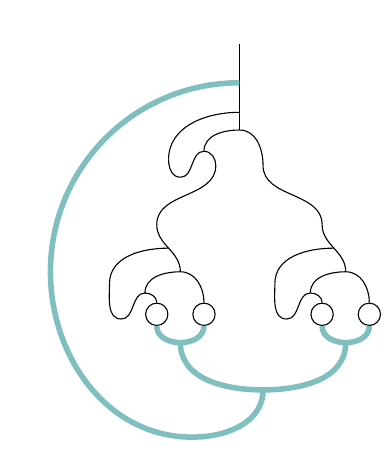
\begin{tikzpicture}[scale=0.3,auto,inner sep=1mm,baseline=(current  bounding  box.center)]
\coordinate (topr) at (0,2); % top of the bottom promoted 2
%\coordinate (comp) at (0,4) {};
\node (vtop) at ($ (topr) + (0,8) $) {};
\coordinate (meet) at ($ (vtop) - (0,2) $); % where the curved !( A -o A ) arc meets at the top

\draw (meet) to (vtop);

% ----------The Church 2 on top
\coordinate (2o) at ($ (topr) + (0,4) $);
\coordinate (2left_meet) at ($ (2o) - (1.5, 0.9) $);
\draw[out=90,in=180] (2left_meet) to (2o);

% Coproduct and derelictions
\coordinate (2R) at ($ (2o) + (1,-1.5) $);
\coordinate (2L) at ($ (2o) + (-1,-1.5) $);
\draw[out=90,in=0] (2R) to (2o);

% The A line curl from bottom to top
\coordinate (2left_curve) at ($ (2o) - (2.5, 2) $);
\coordinate (2left_curve_mid) at ($ (2o) - (3,1.25) $);
\coordinate (2first_meeting_top) at ($ (2o) + (0,0.75) $);
\draw[out=90,in=0] (2L) to (2left_meet);
\draw[out=0,in=180] (2left_curve) to (2left_meet);
\draw[out=180,in=270] (2left_curve) to (2left_curve_mid);
\draw[out=90,in=180] (2left_curve_mid) to (2first_meeting_top);
\draw (2o) to (meet);

%\draw[out=90,in=270] (2join_at_top) to (meet);
\draw[out=90,in=270] ($ (topr) + (-3.5,0) $) to (2L);
\draw[out=90,in=270] ($ (topr) + (3.5,0) $) to (2R);

% -------- promoted 2 LEFT ---------
% All coordinates are relative to the composition vertex (o), which itself
% has its coordinates derived from topr. This is the only link to the outside namespace.
\coordinate (o) at ($ (topr) + (-2.5,-2) $);
\coordinate (elbow) at ($ (o) - (3, 0.5) $);
\coordinate (top_of_circle) at ($ (o) + (-1,2) $);
\dernode (R) at ($ (o) + (1, -1.8) $) {}; % right dereliction
\dernode (L) at ($ (o) - (1,1.8) $) {}; % left dereliction
\coordinate (left_curve) at ($ (o) - (2.5,2) $);
\coordinate (left_meet) at ($ (o) - (1.5, 0.9) $);
\coordinate (delta) at ($ (o) - (0, 3) $); % coproduct vertex
\draw[out=90,in=0] (R) to node [swap] {} (o);
\drawbang[out=0,in=270] (delta) to (R);
\drawbang[out=180,in=270] (delta) to (L);
\draw[out=90,in=180] (left_meet) to (o);
\draw[out=90,in=0] (L) to (left_meet);
\draw[out=0,in=180] (left_curve) to (left_meet);
\draw[out=180,in=270] (left_curve) to (elbow);
\draw[out=90,in=270] (o) to (top_of_circle);
\draw[out=90,in=180] (elbow) to ($ (o)!.5!(top_of_circle) $);
% ------ end promoted 2 ------

% -------- promoted 2 RIGHT ---------
% All coordinates are relative to the composition vertex (o), which itself
% has its coordinates derived from topr. This is the only link to the outside namespace.
\coordinate (o) at ($ (topr) + (4.5,-2) $);
\coordinate (elbow) at ($ (o) - (3, 0.5) $);
\coordinate (top_of_circle) at ($ (o) + (-1,2) $);
\dernode (R) at ($ (o) + (1, -1.8) $) {}; % right dereliction
\dernode (L) at ($ (o) - (1,1.8) $) {}; % left dereliction
\coordinate (left_curve) at ($ (o) - (2.5,2) $);
\coordinate (left_meet) at ($ (o) - (1.5, 0.9) $);
\coordinate (right_delta) at ($ (o) - (0, 3) $); % coproduct vertex
\draw[out=90,in=0] (R) to node [swap] {} (o);
\drawbang[out=0,in=270] (right_delta) to (R);
\drawbang[out=180,in=270] (right_delta) to (L);
\draw[out=90,in=180] (left_meet) to (o);
\draw[out=90,in=0] (L) to (left_meet);
\draw[out=0,in=180] (left_curve) to (left_meet);
\draw[out=180,in=270] (left_curve) to (elbow);
\draw[out=90,in=270] (o) to (top_of_circle);
\draw[out=90,in=180] (elbow) to ($ (o)!.5!(top_of_circle) $);
% ------ end promoted 2 ------


% The loop from the bottom of the promoted 2 up to the top
\coordinate (curve) at (-8, 0);
\coordinate (very_bottom_turn) at (-2,-7);
\coordinate (very_bottom_delta) at (1,-5);
\drawbang[out=270,in=180] (curve) to (very_bottom_turn);
\drawbang[out=90,in=180] (curve) to (meet);
\drawbang[out=0,in=270] (very_bottom_turn) to (very_bottom_delta);
\drawbang[out=0,in=270] (very_bottom_delta) to (right_delta);
\drawbang[out=180,in=270] (very_bottom_delta) to (delta);
\end{tikzpicture}
\quad = \quad
% Final TikZ image for Church 4
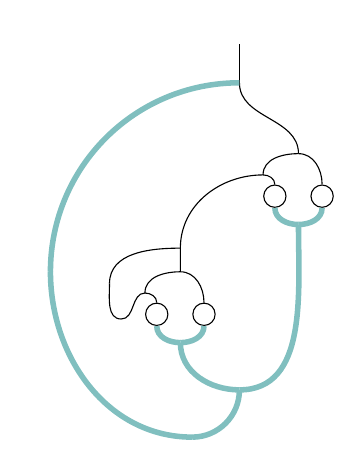
\begin{tikzpicture}[scale=0.3,auto,inner sep=1mm,baseline=(current  bounding  box.center)]
\coordinate (topr) at (0,2); % top of the bottom promoted 2
%\coordinate (comp) at (0,4) {};
\node (vtop) at ($ (topr) + (0,8) $) {};
\coordinate (meet) at ($ (vtop) - (0,2) $); % where the curved !( A -o A ) arc meets at the top

\draw (meet) to (vtop);

% -------- promoted 2 LEFT ---------
% All coordinates are relative to the composition vertex (o), which itself
% has its coordinates derived from topr. This is the only link to the outside namespace.
\coordinate (o) at ($ (topr) + (-2.5,-2) $);
\coordinate (elbow) at ($ (o) - (3, 0.5) $);
\coordinate (top_of_circle) at ($ (o) + (0,1) $);
\dernode (R) at ($ (o) + (1, -1.8) $) {}; % right dereliction
\dernode (L) at ($ (o) - (1,1.8) $) {}; % left dereliction
\coordinate (left_curve) at ($ (o) - (2.5,2) $);
\coordinate (left_meet) at ($ (o) - (1.5, 0.9) $);
\coordinate (delta) at ($ (o) - (0, 3) $); % coproduct vertex
\draw[out=90,in=0] (R) to node [swap] {} (o);
\drawbang[out=0,in=270] (delta) to (R);
\drawbang[out=180,in=270] (delta) to (L);
\draw[out=90,in=180] (left_meet) to (o);
\draw[out=90,in=0] (L) to (left_meet);
\draw[out=0,in=180] (left_curve) to (left_meet);
\draw[out=180,in=270] (left_curve) to (elbow);
\draw[out=90,in=270] (o) to (top_of_circle);
\draw[out=90,in=180] (elbow) to (top_of_circle);
% ------ end promoted 2 ------

% -------- promoted 2 RIGHT ---------
% All coordinates are relative to the composition vertex (o), which itself
% has its coordinates derived from topr. This is the only link to the outside namespace.
\coordinate (o) at ($ (topr) + (2.5,3) $);
\coordinate (elbow) at ($ (o) - (3, 0.5) $);
\coordinate (right_top_of_circle) at ($ (o) + (-1,2) $);
\dernode (R) at ($ (o) + (1, -1.8) $) {}; % right dereliction
\dernode (L) at ($ (o) - (1,1.8) $) {}; % left dereliction
\coordinate (left_curve) at ($ (o) - (2.5,2) $);
\coordinate (left_meet) at ($ (o) - (1.5, 0.9) $);
\coordinate (right_delta) at ($ (o) - (0, 3) $); % coproduct vertex
\draw[out=90,in=0] (R) to node [swap] {} (o);
\drawbang[out=0,in=270] (right_delta) to (R);
\drawbang[out=180,in=270] (right_delta) to (L);
\draw[out=90,in=180] (left_meet) to (o);
\draw[out=90,in=0] (L) to (left_meet);
% ------ end promoted 2 ------

\draw[out=90,in=180] (top_of_circle) to (left_meet);
\draw[out=90,in=270] (o) to (meet);

% The loop from the bottom of the promoted 2 up to the top
\coordinate (curve) at (-8, 0);
\coordinate (very_bottom_turn) at (-2,-7);
\coordinate (very_bottom_delta) at (0,-5);
\drawbang[out=270,in=180] (curve) to (very_bottom_turn);
\drawbang[out=90,in=180] (curve) to (meet);
\drawbang[out=0,in=270] (very_bottom_turn) to (very_bottom_delta);
\drawbang[out=0,in=270] (very_bottom_delta) to (right_delta);
\drawbang[out=180,in=270] (very_bottom_delta) to (delta);
\end{tikzpicture}
\end{equation}
This last diagram is the denotation of $\church{4}_A$, so we conclude that (at least at the level of the denotations) the output of the program $\prf{\mathrm{mult}}_A(2,-)$ on the input $\church{2}_A$ is $\church{4}_A$. The cut-elimination transformations corresponding to these diagram manipulations are given in Appendix \ref{section:appendix_cut_elim}.

\section{Second-order linear logic}\label{section:second}

A measure of the strength or expressiveness of a logic is the class of functions $\mathbb{N} \lto \mathbb{N}$ that can be encoded as proofs. In first-order intuitionistic linear logic $\ILL$ we have already seen how to encode multiplication by an integer as a proof (Definition \ref{definition:mult_m}) and addition will be addressed below (Example \ref{example:addition}) so we deduce that for any formula $A$, any polynomial function $f: \mathbb{N} \lto \mathbb{N}$ may be encoded as a proof of
\begin{equation}\label{eq:intatointa}
\inta_A \vdash \inta_A\,.
\end{equation}
More precisely, for any polynomial function $f$ there exists a proof $F$ of the above sequent with the property that for any integer $n \ge 0$, the cut of $F$ against $\church{n}_A$ reduces under cut-elimination to $\underline{f(n)}_A$. This is close to being a complete list of the functions $f$ that can be encoded as proofs of the sequent \eqref{eq:intatointa}, which comes as a bit of a disappointment~\cite{schwicht}. However, the good news is that more expressive power can be obtained if we allow ourselves to use proofs of $\inta_B \vdash \inta_A$ where $B$ is somehow constructed from $A$. For example, we will see below how to encode exponentials using $B = \inta_A$. 

A very expressive system can be obtained by allowing the base type $B$ to be computed from $A$ at ``run time'', that is, during cut-elimination. This is achieved by adding quantifiers to the language of $\ILL$, and the resulting logic is called \emph{second-order intuitionistic linear logic} $\ILL_2$. One indication of the expressiveness of this extension is that System F \cite[\S 11]{girard_prooftypes} otherwise known as the polymorphic $\lambda$-calculus, embeds into $\ILL_2$ \cite[\S 5.2]{girard_llogic}. These systems have a growing influence on practical programming languages: for example the language Haskell compiles internally to an extension of System F. 
\\

% Perhaps one of the best reasons to care about second-order linear logic is that it makes possible a principled and very exciting perspective on computational complexity \cite{??} which ought to have interesting interactions with algebra and other parts of mathematics.

Our aim in this section is to begin by writing down some more arithmetic in $\ILL$, and then to show how iteration on higher types leads naturally to the need for quantifiers in order to properly represent towers of exponentials. The semantics of $\ILL_2$ is much less clear than the propositional case so we will not speak about it here, but see \cite{girard_systemf,seely_systemf, seely}.

The following examples are taken from \cite[\S 5.3.2]{girard_llogic} and \cite[\S 4]{danos}.

\begin{definition} We define $\prf{\mathrm{comp}}_A$ to be the proof 
\begin{center}
\AxiomC{}
\UnaryInfC{$A \vdash A$}
\AxiomC{}
\UnaryInfC{$A \vdash A$}
\AxiomC{}
\UnaryInfC{$A \vdash A$}
\RightLabel{\scriptsize$\multimap L$}
\BinaryInfC{$A, A \multimap A \vdash A$}
\RightLabel{\scriptsize$\multimap L$}
\BinaryInfC{$A, A \multimap A, A \multimap A \vdash A$}
\RightLabel{\scriptsize$\multimap R$}
\UnaryInfC{$A \multimap A, A \multimap A \vdash A \multimap A$}
\DisplayProof
\qquad
\tagarray{\label{proof_comp}}
\end{center}
As discussed in Remark \ref{example:church_2} the denotation of this proof is the function which \emph{composes} two endomorphisms of  $\den{A}$.
\end{definition}

\begin{example}[(Addition)]\label{example:addition} We define $\prf{\mathrm{add}}_A$ to be the proof (writing $E = A \multimap A$)
\begin{center}
\AxiomC{}
\UnaryInfC{${!}E \vdash {!}E$}
\AxiomC{}
\UnaryInfC{${!}E \vdash {!}E$}
\AxiomC{$\prf{\mathrm{comp}}_A$}
\noLine\UnaryInfC{$\vdots$}
\def\extraVskip{5pt}
\noLine\UnaryInfC{$E, E \vdash E$}
\RightLabel{\scriptsize$\multimap L$}
\BinaryInfC{${!}E, E, \inta_A \vdash E$}
\RightLabel{\scriptsize$\multimap L$}
\BinaryInfC{${!} E, {!} E, \inta_A, \inta_A \vdash E$}
\RightLabel{\scriptsize ctr}
\UnaryInfC{${!} E, \inta_A, \inta_A \vdash E$}
\RightLabel{\scriptsize$\multimap R$}
\UnaryInfC{$\inta_A, \inta_A \vdash \inta_A$}
\DisplayProof
\qquad
\tagarray{\label{add_prooftree}}
\end{center}
which encodes addition on $A$-integers in the following sense: if $\prf{\mathrm{add}}_A$ is cut against two proofs $\church{m}_A$ and $\church{n}_A$ the resulting proof is equivalent under cut-elimination to $\church{m+n}_A$. 

Let us call the result of the cut $\prf{\mathrm{add}}_A( m, n )$, which is a proof of $\inta_A$. One way to see that this reduces to $\underline{m+n}_A$ without laboriously performing cut-elimination by hand is to use a term calculus, as presented in for example \cite{abramsky, benton_etal} or \cite[\S 4]{danos}, to understand the computational content of the proof. Alternatively, with the vector space semantics in mind, one can understand the proof as follows: given a vacuum $\vacu_\alpha$ at an endomorphism $\alpha$ of $V = \den{A}$, the contraction step duplicates this to $\vacu_\alpha \otimes \vacu_\alpha$. The left hand copy of $\vacu_\alpha$ is fed into $\underline{m}_A$ yielding $\alpha^m$ and the right hand copy is fed into $\underline{n}_A$ yielding $\alpha^n$. Then the composition ``machine'' composes these outputs to yield $\alpha^{m+n}$.
\end{example}

To generate a hierarchy of increasingly complex proofs from addition and multiplication we employ \emph{iteration}.

\begin{example}[(Iteration)]\label{example:proof_iteration} Given a proof $\beta$ of $A$ and $\beta'$ of $A \multimap A$ we define $\prf{\mathrm{rec}}_A(\beta, \beta')$ to be the proof
\begin{center}
\AxiomC{$\beta'$}
\noLine\UnaryInfC{$\vdots$}
\def\extraVskip{5pt}
\noLine\UnaryInfC{$\vdash A \multimap A$}
\RightLabel{\scriptsize prom}
\UnaryInfC{$\vdash {!}(A \multimap A)$}
\def\extraVskip{2pt}
\AxiomC{$\beta$}
\noLine\UnaryInfC{$\vdots$}
\def\extraVskip{5pt}
\noLine\UnaryInfC{$\vdash A$}
\AxiomC{}
\UnaryInfC{$A \vdash A$}
\RightLabel{\scriptsize$\multimap L$}
\BinaryInfC{$A \multimap A \vdash A$}
\RightLabel{\scriptsize$\multimap L$}
\BinaryInfC{$\inta_A \vdash A$}
\DisplayProof
\qquad
\tagarray{\label{iteration_prooftree}}
\end{center}
Cut against $\church{n}_A$ this is equivalent under cut-elimination to the $n$th power of $\beta'$ applied to $\beta$, that is, $n$ copies of $\beta'$ cut against one another and then cut against $\beta$.
\end{example}

This game gets more interesting when we get to exponentials. From Definition \ref{definition:mult_m} we know how to define a proof $\prf{\mathrm{mult}}_A(m,-)$ whose cut against $\church{n}_A$ yields something equivalent under cut-elimination to $\church{mn}_A$. But how do we construct a proof which, when cut against $\church{n}_A$, yields a proof equivalent to $\church{m^n}_A$? Naturally we can iterate multiplication by $m$, but the catch is that this requires integers of type $\inta_{\inta_A}$, as we will see in the next example.

\begin{example}[(Exponentials)]\label{example:exponentials} We define
\[
\prf{\mathrm{exp}}_{A,m} = \prf{\mathrm{rec}}_{\inta_A}\big( \church{1}_{A}, \prf{\mathrm{mult}}_A(m,-) \big)\,.
\]
That is,
\begin{center}
\AxiomC{$\prf{\mathrm{mult}}_A(m,-)$}
\noLine\UnaryInfC{$\vdots$}
\def\extraVskip{5pt}
\noLine\UnaryInfC{$\vdash \inta_A \multimap \inta_A$}
\RightLabel{\scriptsize prom}
\UnaryInfC{$\vdash {!}(\inta_A \multimap \inta_A)$}
\def\extraVskip{2pt}
\AxiomC{$\church{1}_{A}$}
\noLine\UnaryInfC{$\vdots$}
\def\extraVskip{5pt}
\noLine\UnaryInfC{$\vdash \inta_A$}
\AxiomC{}
\UnaryInfC{$\inta_A \vdash \inta_A$}
\RightLabel{\scriptsize$\multimap L$}
\BinaryInfC{$\inta_A \multimap \inta_A \vdash \inta_A$}
\RightLabel{\scriptsize$\multimap L$}
\BinaryInfC{$\inta_{\inta_A} \vdash \inta_A$}
\DisplayProof
\qquad
\tagarray{\label{exp_prooftree}}
\end{center}
Cut against $\church{n}_{\inta_A}$ this yields the desired numeral $\church{m^n}_A$.
\end{example}

We begin to see the general pattern: to represent more complicated functions $\mathbb{N} \lto \mathbb{N}$ we need to use more complicated base types $B$ for the integers $\inta_B$ on the left hand side. At the next step, when we try to iterate exponentials, we see that it is hopeless to continue without introducing a way to parametrise over these base types, and this is the role of quantifiers in second-order logic.

To motivate the extension of linear logic to second-order, consider the iteration of the function $n \mapsto 2^n$ which yields a tower of exponentials of variable height. More precisely, $E: \mathbb{N} \lto \mathbb{N}$ is defined recursively by $E(0) = 1, E(n+1) = 2^{E(n)}$ so that
\begin{equation}\label{eq:tower_of_exps_E}
E(n) = 2^{2^{2^{\iddots^{2}}}}
\end{equation}
where the total number of occurrences of $2$ on the right hand side is $n$. To represent the function $E$ as a proof in linear logic we need to introduce integer types with iterated subscripts by the recursive definition
\[
\inta_A(0) = \inta_A, \qquad \inta_A(r+1) =\inta_{\inta_A(r)}\,.
\]
By iteration of the exponential we mean the cut of the following sequence:
\begin{center}
\begin{tabular}{ >{\centering}m{3cm} >{\centering}m{2cm} >{\centering}m{3cm} >{\centering}m{3cm} >{\centering}m{2cm}}
\AxiomC{$\prf{\mathrm{exp}}_{\inta_A(n-1),2}$}
\noLine\UnaryInfC{$\vdots$}
\def\extraVskip{5pt}
\noLine\UnaryInfC{$\inta_A(n+1) \vdash \inta_A(n)$}
\DisplayProof

&

$\cdots$

&

\AxiomC{$\prf{\mathrm{exp}}_{\inta_{A},2}$}
\noLine\UnaryInfC{$\vdots$}
\def\extraVskip{5pt}
\noLine\UnaryInfC{$\inta_{\inta_{\inta_A}} \vdash \inta_{\inta_A}$}
\DisplayProof

&

\AxiomC{$\prf{\mathrm{exp}}_{A,2}$}
\noLine\UnaryInfC{$\vdots$}
\def\extraVskip{5pt}
\noLine\UnaryInfC{$\inta_{\inta_A} \vdash \inta_A$}
\DisplayProof

&
\tagarray{\label{seriesofexponentials}}
\end{tabular}
\end{center}
This yields a proof of $\inta_A(n+1) \vdash \inta_A$ which, when cut against $\church{n}_{\inta_A(n)}$, yields a proof equivalent under cut-elimination to $\church{E(n)}_A$. However this proof is constructed ``by hand'' for each integer $n$. It is clear that what we are doing in essence is iterating the exponential function, but we cannot express this formally in the language of propositional linear logic because the base type on our integers changes from iteration to iteration. To resolve this dilemma we will have to enrich the language by adding quantifiers, after which we will return in Lemma \ref{lemma:hypexp} to the problem of encoding towers of exponentials as proofs.

\begin{definition}[(Second-order linear logic)] The formulas of \emph{second-order linear logic} are defined recursively as follows: any formula of propositional linear logic is a formula, and if $A$ is a formula then so is $\forall x \,.\, A$ for any propositional variable $x$. There are two new deduction rules:
\begin{center}
\begin{tabular}{ >{\centering}m{4cm} >{\centering}m{4cm} }
\AxiomC{$\Gamma \vdash A$}
\RightLabel{\scriptsize$\forall R$}
\UnaryInfC{$\Gamma \vdash \forall x \,.\, A$}
\DisplayProof

&

\AxiomC{$\Gamma, A[B/x] \vdash C$}
\RightLabel{\scriptsize$\forall L$}
\UnaryInfC{$\Gamma, \forall x \,.\, A \vdash C$}
\DisplayProof
\end{tabular}
\end{center}
where $\Gamma$ is a sequence of formulas, possibly empty, and in the right introduction rule we require that $x$ is not free in any formula of $\Gamma$. Here $A[B/x]$ means a formula $A$ with all free occurrences of $x$ replaced by a formula $B$ (as usual, there is some chicanery necessary to avoid free variables in $B$ being captured, but we ignore this).
\end{definition}

Intuitively, the right introduction rule takes a proof $\pi$ and ``exposes'' the variable $x$, for which any type may be substituted. The left introduction rule, dually, takes a formula $B$ in some proof and binds it to a variable $x$. The result of cutting a right introduction rule against a left introduction rule is that the formula $B$ will be bound to $x$ throughout the proof $\pi$. That is, cut-elimination transforms
\begin{center}
\AxiomC{$\pi$}
\noLine\UnaryInfC{$\vdots$}
\def\extraVskip{5pt}
\noLine\UnaryInfC{$\Gamma \vdash A$}
\RightLabel{\scriptsize $\forall R$}
\UnaryInfC{$\Gamma \vdash \forall x \,.\, A$}
\def\extraVskip{2pt}
\AxiomC{$\rho$}
\noLine\UnaryInfC{$\vdots$}
\def\extraVskip{5pt}
\noLine\UnaryInfC{$\Delta, A[B/x] \vdash C$}
\RightLabel{\scriptsize $\forall L$}
\UnaryInfC{$\Delta, \forall x \,.\, A \vdash C$}
\RightLabel{\scriptsize cut}
\BinaryInfC{$\Gamma, \Delta \vdash C$}
\DisplayProof
\qquad
\tagarray{\label{quantifier_before}}
\end{center}
to the proof
\begin{center}
\AxiomC{$\pi[B/x]$}
\noLine\UnaryInfC{$\vdots$}
\def\extraVskip{5pt}
\noLine\UnaryInfC{$\Gamma \vdash A[B/x]$}
\def\extraVskip{2pt}
\AxiomC{$\rho$}
\noLine\UnaryInfC{$\vdots$}
\def\extraVskip{5pt}
\noLine\UnaryInfC{$\Delta, A[B/x] \vdash C$}
\RightLabel{\scriptsize cut}
\BinaryInfC{$\Gamma, \Delta \vdash C$}
\DisplayProof
\qquad
\tagarray{\label{quantifier_after}}
\end{center}
where $\pi[B/x]$ denotes the result of replacing all occurrences of $x$ in the proof $\pi$ with $B$. In the remainder of this section we provide a taste of just what an \emph{explosion} of possibilities the addition of quantifiers to the language represents. 

\begin{example}[(Integers)] The type of integers is
\[
\inta = \forall x \,.\, {!}(x \multimap x) \multimap (x \multimap x)\,.
\]
For each integer $n \ge 0$ we define $\church{n}$ to be the proof
\begin{center}
\AxiomC{$\church{n}_x$}
\noLine\UnaryInfC{$\vdots$}
\def\extraVskip{5pt}
\noLine\UnaryInfC{$\vdash \inta_x$}
\RightLabel{\scriptsize$\forall R$}
\UnaryInfC{$\vdash \inta$}
\DisplayProof
\end{center}
\end{example}

% Notice that for any formula $B$, we have $\inta_B = \inta_x[B/x]$, so that if we have a proof with hypothesis $\inta_B$ we can apply the left introduction rule for $\forall$ to convert this to $\inta$.

\begin{example}[(Exponentials)] We define $\prf{\mathrm{exp}}_m$ to be
\begin{center}
\AxiomC{$\prf{\mathrm{exp}}_{x,m}$}
\noLine\UnaryInfC{$\vdots$}
\def\extraVskip{5pt}
\noLine\UnaryInfC{$\inta_{\inta_x} \vdash \inta_x$}
\RightLabel{\scriptsize$\forall L$}
\UnaryInfC{$\inta \vdash \inta_x$}
\RightLabel{\scriptsize$\forall R$}
\UnaryInfC{$\inta \vdash \inta$}
\DisplayProof
\end{center}
% Notice that the left introduction rule must precede the right introduction rule, because of the requirement that $x$ not be free on the left hand side in the latter rule.
\end{example}

\begin{example}[(Hyper-exponentials)] We define $\prf{\mathrm{hypexp}}$ to be
\begin{center}
\AxiomC{$\prf{\mathrm{exp}}_2$}
\noLine\UnaryInfC{$\vdots$}
\def\extraVskip{5pt}
\noLine\UnaryInfC{$\inta \vdash \inta$}
\RightLabel{\scriptsize $\multimap R$}
\UnaryInfC{$\vdash \inta \multimap \inta$}
\RightLabel{\scriptsize prom}
\UnaryInfC{$\vdash {!}(\inta \multimap \inta)$}
\def\extraVskip{2pt}
\AxiomC{$\church{1}$}
\noLine\UnaryInfC{$\vdots$}
\def\extraVskip{5pt}
\noLine\UnaryInfC{$\vdash \inta$}
\AxiomC{}
\UnaryInfC{$\inta \vdash \inta$}
\RightLabel{\scriptsize$\multimap L$}
\BinaryInfC{$\inta \multimap \inta \vdash \inta$}
\RightLabel{\scriptsize$\multimap L$}
\BinaryInfC{$\inta_{\inta} \vdash \inta$}
\RightLabel{\scriptsize $\forall L$}
\UnaryInfC{$\inta \vdash \inta$}
\DisplayProof
\qquad
\tagarray{\label{hyperexp_prooftree}}
\end{center}
\end{example}

\begin{lemma}\label{lemma:hypexp} The cut of $\church{n}$ against $\prf{\mathrm{hypexp}}$ reduces to $\church{E(n)}$.
\end{lemma}
\begin{proof}
We sketch how $\prf{\mathrm{hypexp}} \l \church{2}$ reduces to the sequence of cuts in \eqref{seriesofexponentials}, since the argument for general $n$ is similar. The first reduction is of the cut of left and right introduction rules for the quantifier \eqref{quantifier_before} $\rightsquigarrow$ \eqref{quantifier_after} which leaves a cut of $\church{2}_{\inta}$ against the proof \eqref{hyperexp_prooftree} up to its penultimate step. The second reduction is \eqref{eq:cutelim3} $\rightsquigarrow$ \eqref{eq:cutelim4}, i.e. \cite[\S 3.8.2]{mellies}, to
\begin{center}
\AxiomC{$\prf{\mathrm{exp}}_2$}
\noLine\UnaryInfC{$\vdots$}
\def\extraVskip{5pt}
\noLine\UnaryInfC{$\inta \vdash \inta$}
\RightLabel{\scriptsize $\multimap R$}
\UnaryInfC{$\vdash \inta \multimap \inta$}
\RightLabel{\scriptsize prom}
\UnaryInfC{$\vdash {!}(\inta \multimap \inta)$}
\def\extraVskip{2pt}
\AxiomC{$\church{2}_{\inta}$}
\noLine\UnaryInfC{$\vdots$}
\def\extraVskip{5pt}
\noLine\UnaryInfC{${!}( \inta \multimap \inta) \vdash \inta \multimap \inta$}
\RightLabel{\scriptsize cut}
\BinaryInfC{$\vdash \inta \multimap \inta$}
\AxiomC{$\church{1}$}
\noLine\UnaryInfC{$\vdots$}
\def\extraVskip{5pt}
\noLine\UnaryInfC{$\vdash \inta$}
\AxiomC{}
\UnaryInfC{$\inta \vdash \inta$}
\RightLabel{\scriptsize$\multimap L$}
\BinaryInfC{$\inta \multimap \inta \vdash \inta$}
\RightLabel{\scriptsize cut}
\BinaryInfC{$\vdash \inta$}
\DisplayProof
\quad
\tagarray{\label{hyperexp_prooftree_hyp}}
\end{center}
The left hand branch of this proof is familiar from Example \ref{example:cutagainst2}, so we know it reduces to the square of $\prf{\mathrm{exp}}_2$ which we can write as
\begin{center}
\AxiomC{$\prf{\mathrm{exp}}_{y,2}$}
\noLine\UnaryInfC{$\vdots$}
\def\extraVskip{5pt}
\noLine\UnaryInfC{$\inta_{\inta_y} \vdash \inta_y$}
\RightLabel{\scriptsize$\forall L$}
\UnaryInfC{$\inta \vdash \inta_y$}
\RightLabel{\scriptsize$\forall R$}
\UnaryInfC{$\inta \vdash \inta$}
\def\extraVskip{2pt}
\AxiomC{$\prf{\mathrm{exp}}_{x,2}$}
\noLine\UnaryInfC{$\vdots$}
\def\extraVskip{5pt}
\noLine\UnaryInfC{$\inta_{\inta_x} \vdash \inta_x$}
\RightLabel{\scriptsize$\forall L$}
\UnaryInfC{$\inta \vdash \inta_x$}
\RightLabel{\scriptsize$\forall R$}
\UnaryInfC{$\inta \vdash \inta$}
\RightLabel{\scriptsize cut}
\BinaryInfC{$\inta \vdash \inta$}
\DisplayProof
\quad
\tagarray{\label{hyperexp_quant}}
\end{center}
followed by a right introduction rule to get a proof of $\vdash \inta \multimap \inta$. There is a cut-elimination transformation that allows us to commute the cut past the right introduction rule in the right branch. At that point the right introduction rule (in the left branch) is cut against the left introduction rule (in the right branch) and the rewrite \eqref{quantifier_before} $\rightsquigarrow$ \eqref{quantifier_after} transforms this to a substitution of $y = \inta_x$ in the left branch:
\begin{center}
\AxiomC{$\prf{\mathrm{exp}}_{\inta_x,2}$}
\noLine\UnaryInfC{$\vdots$}
\def\extraVskip{5pt}
\noLine\UnaryInfC{$\inta_{\inta_{\inta_x}} \vdash \inta_{\inta_x}$}
\RightLabel{\scriptsize$\forall L$}
\UnaryInfC{$\inta \vdash \inta_{\inta_x}$}
\def\extraVskip{2pt}
\AxiomC{$\prf{\mathrm{exp}}_{x,2}$}
\noLine\UnaryInfC{$\vdots$}
\def\extraVskip{5pt}
\noLine\UnaryInfC{$\inta_{\inta_x} \vdash \inta_x$}
\RightLabel{\scriptsize cut}
\BinaryInfC{$\inta \vdash \inta_x$}
\RightLabel{\scriptsize$\forall R$}
\UnaryInfC{$\inta \vdash \inta$}
\DisplayProof
\quad
\tagarray{\label{hyperexp_quant2}}
\end{center}
This is enough to show that the proof $\prf{\mathrm{hypexp}} \l \church{2}$ reduces to the first two cuts in \eqref{seriesofexponentials}.
\end{proof}

Once we have added quantifiers, the expressive power of the language is immense. We can for example easily iterate hyper-exponentials to obtain a tower of exponentials whose height is itself a tower of exponentials, and by iterating at the type $\inta \multimap \inta$ obtain monsters like the Ackermann function \cite[\S 6.D]{girard_blindspot}. More precisely:

\begin{theorem}[Girard] Any recursive function $\mathbb{N} \lto \mathbb{N}$ which is provably total in second-order Peano arithmetic can be encoded into second-order linear logic as a proof of the sequent $\inta \vdash \inta$.
\end{theorem}
\begin{proof}
See \cite[\S 15.2]{girard_prooftypes} and \cite[\S 5.3.2]{girard_llogic}.
\end{proof}
% The functions representable in F are exactly those which are provably total in PA2.

\appendix

\section{Example of cut-elimination}\label{section:appendix_cut_elim}

We examine the beginning of the cut-elimination process applied to the proof \eqref{cut_mult_2}. Our reference for cut-elimination is Melli\`{e}s \cite[\S 3.3]{mellies}. Throughout a formula $A$ is fixed and we write $E = A \multimap A$ so that $\inta_A = {!}E \multimap E$. We encourage the reader to put the following series of proof trees side-by-side with the evolving diagrams in \eqref{cut_mult_2}-\eqref{diagram_mult_2_3} to see the correspondence between cut-elimination and diagram manipulation.

To begin, we expose the first layer of structure within $\prf{\mathrm{mult}}_A(2,-)$ to obtain
\begin{center}
\AxiomC{$\church{2}_A$}
\noLine\UnaryInfC{$\vdots$}
\def\extraVskip{5pt}
\noLine\UnaryInfC{$\vdash \inta_A$}
\def\extraVskip{2pt}
\AxiomC{$\prf{\mathrm{mult}}_A(2,-)$}
\noLine\UnaryInfC{$\vdots$}
\def\extraVskip{5pt}
\noLine\UnaryInfC{$!E, \inta_A \vdash E$}
\def\extraVskip{2pt}
\RightLabel{\scriptsize $\multimap R$}
\UnaryInfC{$\inta_A \vdash \inta_A$}
\RightLabel{\scriptsize cut}
\BinaryInfC{$\vdash \inta_A$}
\DisplayProof
\qquad
\tagarray{\label{cut_step_1}}
%\begin{tikzpicture}[scale=0.6,auto]
%\node (topr) at (1,4) {$\inta_A$};
%\bluenode (o) at (1,0) {};
%\bluenode (gam) at (2.5,-2) {};
%\draw[out=90,in=0] (gam) to node [swap]{$\inta_A$} (o);
%\drawbang[out=0,in=180] (-1.5,-2) to node {} (o);
%\drawbang[out=180,in=270] (-1.5,-2) to (-3,0);
%\drawbang[out=90,in=180] (-3,0) to (1,2);
%\draw (o) to node [swap] {$E$} (1,2);
%\draw (1,2) to (topr);
%\end{tikzpicture}
%\end{tabular}
\end{center}
For a cut against a proof whose last deduction rule is a right introduction rule for $\multimap$, the cut elimination procedure \cite[\S 3.11.10]{mellies} prescribes that \eqref{cut_step_1} be transformed to
\begin{center}
\AxiomC{$\church{2}_A$}
\noLine\UnaryInfC{$\vdots$}
\def\extraVskip{5pt}
\noLine\UnaryInfC{$\vdash \inta_A$}
\def\extraVskip{2pt}
\AxiomC{$\prf{\mathrm{mult}}_A(2,-)$}
\noLine\UnaryInfC{$\vdots$}
\def\extraVskip{5pt}
\noLine\UnaryInfC{$!E, \inta_A \vdash E$}
\def\extraVskip{2pt}
\RightLabel{\scriptsize cut}
\BinaryInfC{$!E \vdash E$}
\RightLabel{\scriptsize $\multimap R$}
\UnaryInfC{$\vdash \inta_A$}
\DisplayProof
\qquad
\tagarray{\label{cut_step_2}}
\end{center}
If we fill in the content of $\prf{\mathrm{mult}}_A(2,-)$, this proof may be depicted as follows:
\begin{center}
\AxiomC{$\church{2}_A$}
\noLine\UnaryInfC{$\vdots$}
\def\extraVskip{5pt}
\noLine\UnaryInfC{$!E  \vdash E$}
\def\extraVskip{2pt}
\UnaryInfC{$\vdash \inta_A$}
\AxiomC{$\church{2}_A$}
\noLine\UnaryInfC{$\vdots$}
\def\extraVskip{5pt}
\noLine\UnaryInfC{$!E \vdash E$}
\def\extraVskip{2pt}
\RightLabel{\scriptsize prom}
\UnaryInfC{$!E \vdash {!}E$}
\AxiomC{}
\UnaryInfC{$E \vdash E$}
\RightLabel{\scriptsize$\multimap L$}
\BinaryInfC{$!E, \inta_A \vdash E$}
\RightLabel{\scriptsize cut}
\BinaryInfC{$!E \vdash E$}
\RightLabel{\scriptsize $\multimap R$}
\UnaryInfC{$\vdash \inta_A$}
\DisplayProof
\qquad
\tagarray{\label{cut_step_3}}
\end{center}
The next cut-elimination step \cite[\S 3.8.2]{mellies} transforms this proof to
\begin{center}
\AxiomC{$\church{2}_A$}
\noLine\UnaryInfC{$\vdots$}
\def\extraVskip{5pt}
\noLine\UnaryInfC{$!E \vdash E$}
\def\extraVskip{2pt}
\RightLabel{\scriptsize prom}
\UnaryInfC{$!E \vdash {!}E$}
\AxiomC{$\church{2}_A$}
\noLine\UnaryInfC{$\vdots$}
\def\extraVskip{5pt}
\noLine\UnaryInfC{$!E \vdash E$}
\def\extraVskip{2pt}
\RightLabel{\scriptsize cut}
\BinaryInfC{$!E \vdash E$}
\AxiomC{}
\UnaryInfC{$E \vdash E$}
\RightLabel{\scriptsize cut}
\BinaryInfC{$!E \vdash E$}
\RightLabel{\scriptsize $\multimap R$}
\UnaryInfC{$\vdash \inta_A$}
\DisplayProof
\quad
\tagarray{\label{cut_step_4}}
\end{center}
As may be expected, cutting against an axiom rule does nothing, so this is equivalent to
\begin{prooftree}
\AxiomC{$\church{2}_A$}
\noLine\UnaryInfC{$\vdots$}
\def\extraVskip{5pt}
\noLine\UnaryInfC{$!E \vdash E$}
\def\extraVskip{2pt}
\RightLabel{\scriptsize prom}
\UnaryInfC{$!E \vdash {!}E$}
\AxiomC{$\church{2}_A'$}
\noLine\UnaryInfC{$\vdots$}
\def\extraVskip{5pt}
\noLine\UnaryInfC{$!E, !E \vdash E$}
\def\extraVskip{2pt}
\RightLabel{\scriptsize ctr}
\UnaryInfC{$!E \vdash E$}
\RightLabel{\scriptsize cut}
\BinaryInfC{$!E \vdash E$}
\RightLabel{\scriptsize $\multimap R$}
\UnaryInfC{$\vdash \inta_A$}
\end{prooftree}
where $\church{2}_A'$ is a sub-proof of $\church{2}_A$. Here is the important step: cut-elimination replaces a cut of a promotion against a contraction by a pair of promotions \cite[\S 3.9.3]{mellies}. This step corresponds to the doubling of the promotion box in \eqref{diagram_mult_2_2}
\begin{prooftree}
\AxiomC{$\church{2}_A$}
\noLine\UnaryInfC{$\vdots$}
\def\extraVskip{5pt}
\noLine\UnaryInfC{$!E \vdash E$}
\def\extraVskip{2pt}
\UnaryInfC{$!E \vdash {!}E$}
\AxiomC{$\church{2}_A$}
\noLine\UnaryInfC{$\vdots$}
\def\extraVskip{5pt}
\noLine\UnaryInfC{$!E \vdash E$}
\def\extraVskip{2pt}
\UnaryInfC{$!E \vdash {!}E$}
\AxiomC{$\church{2}_A'$}
\noLine\UnaryInfC{$\vdots$}
\def\extraVskip{5pt}
\noLine\UnaryInfC{$!E, !E \vdash E$}
\def\extraVskip{2pt}
\RightLabel{\scriptsize cut}
\BinaryInfC{$!E, !E \vdash E$}
\RightLabel{\scriptsize cut}
\BinaryInfC{$!E, !E \vdash E$}
\RightLabel{\scriptsize ctr}
\UnaryInfC{$!E \vdash E$}
\RightLabel{\scriptsize $\multimap R$}
\UnaryInfC{$\vdash \inta_A$}
\end{prooftree}
We only sketch the rest of the cut-elimination process: next, the derelictions in $\church{2}_A'$ will be annihilate with the promotions in the two copies of $\church{2}_A$ according to \cite[\S 3.9.1]{mellies}. Then there are numerous eliminations involving the right and left $\multimap$ introduction rules. %, which are not very interesting. %The point is that after the next step, cuts on formulas $!(A \multimap A)$ will be replaced by cuts on formulas $A \multimap A$, which are of lower complexity. 

\section{Tangents and proofs}\label{section:example_lifting}

%In this appendix we consider various examples of the lifting formula in Theorem \ref{theorem:describe_lifting}, centered around the notion of tangent vectors at proof denotations. 


%\begin{definition}\label{defn:nonlinear_deno} Given a proof $\pi$ of a sequent $!A \vdash B$ let $\langle \pi \rangle$ denote the function
%\begin{gather*}
%\langle \pi \rangle: \den{A} \lto \den{B},\\
%\langle \pi \rangle(P) = \den{\pi} \vacu_P\,.
%\end{gather*}
%\end{definition}

%One interesting example of lifting involves tangent vectors at proofs.

\begin{example}\label{example:tangent_coalgebra} Let $\cat{T}$ the coalgebra given by the dual of the finite-dimensional algebra $k[t]/(t^2)$. It has a $k$-basis $1 = 1^*$ and $\varepsilon = t^*$ and coproduct $\Delta$ and counit $u$ defined by
\[
\Delta(1) = 1 \otimes 1, \quad \Delta( \varepsilon ) = 1 \otimes \varepsilon + \varepsilon \otimes 1, \quad u(1) = 1, \quad u(\varepsilon) = 0\,.
\]
Recall that a tangent vector at a point $x$ on a scheme $X$ is a morphism $\Spec(k[t]/t^2) \lto X$ sending the closed point to $x$. Given a finite-dimensional vector space $V$ and $R = \Sym(V^*)$ with $X = \Spec(R)$, this is equivalent to a morphism of $k$-algebras
\[
\varphi: \Sym(V^*) \lto k[t]/t^2
\]
with $\varphi^{-1}( (t) ) = x$. Such a morphism of algebras is determined by its restriction to $V^*$, which as a linear map $\varphi|_{V^*}: V^* \lto k[t]/t^2$ corresponds to a pair of elements $(P, Q)$ of $V$, where $\varphi( \tau ) = \tau(P) \cdot 1 + \tau(Q) \cdot t$. Then $\varphi$ sends a polynomial $f$ to
\[
\varphi(f) = f(P) \cdot 1 + \partial_Q( f )|_P \cdot t\,.
\]
The map $\varphi|_{V^*}$ is also determined by its dual, which is a linear map $\phi: \cat{T} \lto V$. By the universal property, this lifts to a morphism of coalgebras $\Phi: \cat{T} \lto {!}V$. If $\phi$ is determined by a pair of points $(P,Q) \in V^{\oplus 2}$ as above, then it may checked directly that
\[
\Phi( 1 ) = \vacu_P, \qquad \Phi( \varepsilon ) = \ket{ Q }_P
\]
is a morphism of coalgebras lifting $\phi$.
%Using the dual of $k[t]/t^N$ for various powers $N$ we may in this way make an identification between ${!} V$ and the infinite jet-space of $V$.
\end{example}

Motivated by this example, we make a preliminary investigation into tangent vectors at proof denotations. Let $A,B$ be types with finite-dimensional denotations $\den{A}, \den{B}$.

\begin{definition} Given a proof $\pi$ of $\vdash A$ a \emph{tangent vector} at $\pi$ is a morphism of coalgebras $\theta: \cat{T} \lto {!} \den{A}$ with the property that $\theta(1) = \vacu_{\den{\pi}}$, or equivalently that the diagram
\begin{equation}
\xymatrix@C+2pc{
k \ar[d]_-{1} \ar[r]^-{\den{\pi}} & \den{A}\\
\cat{T} \ar[r]_-{\theta} & {!} \den{A} \ar[u]_-{d}
}
\end{equation}
commutes. The set of tangent vectors at $\pi$ is denoted $T_{\pi}$.
\end{definition}

It follows from Example \ref{example:tangent_coalgebra} that there is a bijection
\[
\den{A} \lto T_{\pi}
\]
sending $Q \in \den{A}$ to the coalgebra morphism $\theta$ with $\theta(1) = \vacu_{\den{\pi}}$ and $\theta(\varepsilon) = \ket{Q}_{\den{\pi}}$. We use this bijection to equip $T_{\pi}$ with the structure of a vector space.

Note that the denotation of a program not only maps inputs to outputs (if we identify inputs and outputs with vacuum vectors) but also tangent vectors to tangent vectors. To wit, if $\rho$ is a proof of a sequent $!A \vdash B$ with denotation $\lambda: {!} \den{A} \lto \den{B}$, then composing a tangent vector $\theta$ at a proof $\pi$ of $\vdash A$ with the lifting $\Lambda$ of $\lambda$ leads to a tangent vector at the cut of $\rho$ against the promotion of $\pi$. That is, the linear map
\begin{equation}\label{eq:fake_tangent_map}
\xymatrix@C+2pc{
\cat{T} \ar[r]^-{\theta} & ! \den{A} \ar[r]^-{\Lambda} & ! \den{B}
}
\end{equation}
is a tangent vector at the following proof, which we denote $\rho \l \pi$
\begin{prooftree}
\AxiomC{$\pi$}
\noLine\UnaryInfC{$\vdots$}
\def\extraVskip{5pt}
\noLine\UnaryInfC{$\vdash A$}
\def\extraVskip{2pt}
\RightLabel{\scriptsize prom}
\UnaryInfC{$\vdash {!} A$}
\AxiomC{$\rho$}
\noLine\UnaryInfC{$\vdots$}
\def\extraVskip{5pt}
\noLine\UnaryInfC{$!A \vdash B$}
\def\extraVskip{2pt}
\RightLabel{\scriptsize cut}
\BinaryInfC{$\vdash B$}
\end{prooftree}
By Theorem \ref{theorem:describe_lifting} the linear map of tangent spaces induced in this way by $\rho$ is
\begin{gather}
\den{A} \cong T_{\pi} \lto T_{\rho\l\pi} \cong \den{B}\label{eq:tangent_map_logic}\\
Q \longmapsto \lambda \ket{Q}_{\den{\pi}}\nonumber
\end{gather}

When $\rho$ computes a smooth map of differentiable manifolds, this map can be compared with an actual map of tangent spaces. We examine $\rho = \church{2}_A$ below. It would be interesting to understand these maps in more complicated examples; this seems to be related to the differential $\lambda$-calculus \cite{ehrhard_difflambda,ehrhard_difflambda2}, but we have not tried to work out the precise connection.

\begin{example}\label{example:tangent_to_2} When $k = \mathbb{C}$ and $Z = \den{\church{2}_A}_{nl}$ we have by Lemma \ref{lemma:nonlinear_recover}
\[
Z: M_n(\mathbb{C}) \lto M_n(\mathbb{C}), \qquad Z(\alpha) = \alpha^2\,.
\]
The tangent map of the smooth map of manifolds $Z$ at $\alpha \in M_n(\mathbb{C})$ is $(Z_*)_\alpha( \nu ) = \{ \nu, \alpha \}$. When $\alpha$ is the denotation of some proof $\pi$ of $\vdash A \multimap A$ this agrees with the tangent map assigned in \eqref{eq:tangent_map_logic} to the proof $\church{2}_A$ at $\pi$, using \eqref{eq:church_2_den}.
\end{example}

\bibliographystyle{amsalpha}
\providecommand{\bysame}{\leavevmode\hbox to3em{\hrulefill}\thinspace}
\providecommand{\href}[2]{#2}
\begin{thebibliography}{BHLS03}

\bibitem{abramsky}
S.~Abramsky, \textsl{Computational interpretations of linear logic}, Theoretical Computer Science, 1993.

%\bibitem{abramsky4}
%S.~Abramsky, \textsl{Retracting some paths in process algebra}, In CONCUR 96, Springer Lecture Notes in Computer Science \textbf{1119}, 1--17, 1996.

%\bibitem{abramsky2}
%S.~Abramsky, \textsl{Geometry of {I}nteraction and linear combinatory algebras}, Mathematical Structures in Computer Science, \textbf{12}, 625--665, 2002.

%\bibitem{abramsky3}
%S.~Abramsky and R.~Jagadeesan, \textsl{New foundations for the {G}eometry of {I}nteraction}, Information and Computation \textbf{111} (1), 53--119, 1994.

\bibitem{anel}
M.~Anel, A.~Joyal, \textsl{Sweedler theory of (co)algebras and the bar-cobar constructions}, \href{http://arxiv.org/abs/1309.6952}{[arXiv:1309.6952]}

%\bibitem{atiyah}
%M.~Atiyah, \textsl{Topological quantum field theories}, Publications Math\'{e}matique de l'IH\'{E}S 68, 175--186, 1989.

\bibitem{baez}
J.~Baez and M.~Stay, \textsl{Physics, topology, logic and computation: a Rosetta stone}, in B. Coecke (ed.) New Structures for Physics, Lecture Notes in Physics 813, Springer, Berlin, 95--174, 2011

\bibitem{barr}
M.~Barr, \textsl{Coalgebras over a commutative ring}, Journal of Algebra 32, 600--610, 1974.

\bibitem{barr_auto}
\bysame, \textsl{$\star$-autonomous categories}, Number 752 in Lecture Notes in Mathematics. Springer-Verlag, 1979.

\bibitem{barr_acc}
\bysame, \textsl{Accessible categories and models of linear logic}, Journal of Pure and Applied Algebra, 69(3):219--232, 1990.

\bibitem{barr_autolin}
\bysame, {$\star$-autonomous categories and linear logic}, Mathematical Structures in Computer Science, 1(2):159--178, 1991.

%\bibitem{barr_chu}
%\bysame, \textsl{The {C}hu construction: history of an idea}, Theory and Applications of Categories, Vol. 17, No. 1, 10--16, 2006.

\bibitem{benton_strong}
N.~Benton, \textsl{Strong normalisation for the linear term calculus}, Technical Report 305, Computer Laboratory, University of Cambridge, 1993.

\bibitem{benton}
\bysame, \textsl{A mixed linear and non-linear logic; proofs, terms and models}, in Proceedings of Computer Science Logic 94, vol. 933 of Lecture Notes in Computer Science, Verlag, 1995.

\bibitem{benton_etal}
N.~Benton, G.~Bierman, V.~de Paiva and M.~Hyland, \textsl{Term assignment for intuitionistic linear logic}, Technical report 262, Computer Laboratory, University of Cambridge, 1992.

%\bibitem{block-leroux} 
%R.~Block, P.~Leroux, \textsl{Generalized dual coalgebras of algebras, with applications to cofree coalgebras}, J. Pure Appl. Algebra 36, no. 1, 15--21, 1985.

%\bibitem{blute}
%R.~Blute, \textsl{Hopf algebras and linear logic}, Mathematical Structures in Computer Science, 6(2):189--217, 1996.

%\bibitem{blute_scott}
%R.~Blute and P.~Scott, \textsl{Linear {L}a\"{u}chli semantics}, Annals of Pure and Applied Logic, 77:101--142, 1996.

\bibitem{blue_book}
\bysame, \textsl{Category theory for linear logicians}, Linear Logic in Computer Science 316: 3--65, 2004.

\bibitem{blute_fock}
R.~Blute, P.~Panangaden, R.~Seely, \textsl{Fock space: a model of linear exponential types}, in: Proc. Ninth Conf. on Mathematical Foundations of Programming Semantics, Lecture Notes in Computer Science, Vol. 802, Springer, Berlin, 1--25, 1994.

\bibitem{brauner}
T.~Brauner, \textsl{Introduction to linear logic}, Basic Research in Computer Science, Lecture Notes (1996).

\bibitem{church}
A.~Church, \textsl{The {C}alculi of {L}ambda-conversion}, Princeton University Press, Princeton, N. J. 1941.

\bibitem{danos}
V.~Danos and J.-B.~Joinet, \textsl{Linear logic and elementary time}, Information and Computation 183, 123--127, 2003.

%\bibitem{danos_regnier1}
%V.~Danos and L.~Regnier, \textsl{Local and {A}synchronous beta-reduction (an analysis of {G}irard's execution formula)} in: Springer Lecture Notes in Computer Science \textbf{8}, 296--306, 1993.

%\bibitem{danos_regnier2}
%V.~Danos and L.~Regnier, \textsl{Proof-nets and the Hilbert space}, in (Girard \textsl{et. al.} 1995), 307--328, 1995.

%\bibitem{denning}
%P.~J.~Denning, \textsl{Ubiquity symposium ``What is computation?''}: opening statement, Ubiquity 2010. Available on the \href{http://ubiquity.acm.org/article.cfm?id=1870596}{Ubiquity website}.

%\bibitem{dm1102.2957}
%T.~Dyckerhoff and D.~Murfet, \textsl{Pushing forward matrix factorisations}, Duke Math. J. Volume 162, Number 7 1249--1311, 2013 \href{http://arxiv.org/abs/1102.2957}{[arXiv:1102.2957]}.

\bibitem{ehrhard}
T.~Ehrhard, \textsl{Finiteness spaces}, Math. Structures Comput. Sci. 15 (4) 615--646, 2005.

%\bibitem{ehrhard_kothe}
%\bysame, \textsl{On {K}\"othe sequence spaces and linear logic}, Mathematical Structures in Computer Science 12.05, 579--623, 2002.

\bibitem{ehrhard_difflambda}
T.~Ehrhard and L.~Regnier, \textsl{The differential lambda-calculus}, Theoretical Computer Science 309.1: 1--41, 2003.

\bibitem{ehrhard_difflambda2}
\bysame, \textsl{Differential interaction nets}, Theoretical Computer Science 364.2: 166--195, 2006.

\bibitem{gentzen}
G.~Gentzen, \textsl{The Collected Papers of Gerhard Gentzen}, (Ed. M. E. Szabo), Amsterdam, Netherlands: North-Holland, 1969.

\bibitem{getzler}
E.~Getzler, P.~Goerss, \emph{A model category structure for differential graded coalgebras}, preprint, 1999.
  
\bibitem{girard_systemf}
J.-Y.~Girard, \textsl{The system F of variable types, fifteen years later}, Theoretical Computer Science 45 (1986): 159--192.
  
\bibitem{girard_llogic}
\bysame, \textsl{Linear Logic}, Theoretical Computer Science 50 (1), 1--102, 1987.

\bibitem{girard_normal}
\bysame, \textsl{Normal functors, power series and the $\lambda$-calculus} Annals of Pure and Applied
Logic, 37: 129--177, 1988.

\bibitem{girard_goi1}
\bysame, \textsl{Geometry of {I}nteraction I: {I}interpretation of {S}ystem {F}}, in Logic Colloquium '88, ed. R.~Ferro, et al. North-Holland, 221--260, 1988.

\bibitem{girard_goi2}
\bysame, \textsl{Geometry of {I}nteraction II: {D}eadlock-free {A}lgorithms}, COLOG-88, Springer Lecture Notes in Computer Science \textbf{417}, 76--93, 1988.

\bibitem{girard_towards}
\bysame, \textsl{Towards a geometry of interaction}, In J.~W.~Gray and A.~Scedrov, editors, Categories in Computer Science and Logic, volume 92 of Contemporary Mathematics, 69--108, AMS, 1989.

\bibitem{girard_goi3}
\bysame, \textsl{Geometry of {I}nteraction III: {A}ccommodating the {A}dditives}, in (Girard \textsl{et al}. 1995), pp.1--42.

\bibitem{girard_complexity}
\bysame, \textsl{Light linear logic}, Information and Computation 14, 1995.

\bibitem{girard_synandsem} 
\bysame, \textsl{Linear logic: its syntax and semantics}, London Mathematical Society Lecture Note Series (1995): 1--42.

\bibitem{girard_coherentbanach}
\bysame, \textsl{Coherent {B}anach spaces: a continuous denotational semantics}, Theoretical Computer Science, 227: 275--297, 1999.

\bibitem{girard_blindspot}
\bysame, \textsl{The Blind Spot: lectures on logic}, European Mathematical Society, 2011.

\bibitem{girard_prooftypes}
J.-Y.~Girard, Y.~Lafont, and P.~Taylor, \textsl{Proofs and Types}, Cambridge Tracts in Theoretical Computer Science 7 ,Cambridge University Press, 1989.

\bibitem{Gonthier}
G.~Gontheir, M.~Abadi and J.-J.~L\'{e}vy, \textsl{The geometry of optimal lambda reduction}, in 9th Annual IEEE Symp. on Logic in Computer Science (LICS), 15--26, 1992.
  
\bibitem{haghverdi}
E.~Haghverdi and P.~Scott, \textsl{Geometry of {I}nteraction and the dynamics of prood reduction: a tutorial}, in New Structures for Physics, Lecture notes in Physics \textbf{813}, 357--417, 2011.
  
\bibitem{hazewinkel}
H.~Hazewinkel, \textsl{Cofree coalgebras and multivariable recursiveness}, J. Pure Appl. Algebra 183, no. 1--3, 61--103, 2003.

\bibitem{hyland}
M.~Hyland and A.~Schalk, \textsl{Glueing and orthogonality for models of linear logic}, Theoretical Computer Science, 294: 183--231, 2003.

\bibitem{JSGoTCI}
A.~Joyal and R.~Street, \textsl{The geometry of tensor calculus I}, Advances in Math. \textbf{88}, 55--112, 1991.

\bibitem{JSGoTCII}
A.~Joyal and R.~Street, \textsl{The geometry of tensor calculus II}, 
draft available at 
\href{http://maths.mq.edu.au/~street/GTCII.pdf}{http://maths.mq.edu.au/\textasciitilde street/GTCII.pdf}

\bibitem{joyal_trace}
A.~Joyal, R.~Street and D.~Verity, \textsl{Traced monoidal categories}, Math. Proc. Camb. Phil. Soc. 119, 447--468, 1996.

\bibitem{khovdia}
M.~Khovanov, \textsl{Categorifications from planar diagrammatics}, Japanese J. of Mathematics \textbf{5}, 153--181, 2010 \href{http://arxiv.org/abs/1008.5084}{[arXiv:1008.5084]}.
  
\bibitem{lafont}
Y.~Lafont, \textsl{The {L}inear {A}bstract {M}achine}, Theoretical Computer Science, 59 (1,2):157--180, 1988.

\bibitem{lambek}
J.~Lambek and P.~J.~Scott, \textsl{Introduction to higher order categorical logic}, Cambridge Studies in Advanced Mathematics, vol. 7, Cambridge University Press, Cambridge, 1986.

\bibitem{ladia}
A.~D.~Lauda, \textsl{An introduction to diagrammatic algebra and categorified quantum $\mathfrak{sl}_2$}, Bulletin of the Institute of Mathematics Academia Sinica (New Series), Vol. \textbf{7}, No. 2, 165--270, 2012 \href{http://arxiv.org/abs/1106.2128}{[arXiv:1106.2128]}.

\bibitem{mccarthy}
J.~McCarthy, \textsl{Recursive functions of symbolic expressions and their computation by machine, Part I.}, Communications of the ACM 3.4: 184--195, 1960.

%\bibitem{McNameethesis}
%D.~McNamee, \textsl{On the mathematical structure of topological defects in
%  {L}andau-{G}inzburg models}, MSc Thesis, Trinity College Dublin, 2009.
  
\bibitem{mellies_dia}
P.-A.~Melli\`{e}s, \textsl{Functorial boxes in string diagrams}, In Z. \'{E}sik, editor, Computer Science Logic,
volume 4207 of Lecture Notes in Computer Science, pages 1--30, Springer Berlin / Heidelberg,
2006.

\bibitem{mellies}
P-A.~Melli\`{e}s, \textsl{Categorical semantics of linear logic}, in : Interactive models of computation and program behaviour, Panoramas et Synth\`{e}ses $27$, Soci\'{e}t\'{e} Math\'{e}matique de France, 2009.

\bibitem{mellies2}
P.-A.~Melli\`{e}s, N.~Tabareau, C.~Tasson, \textsl{An explicit formula for the free exponential modality of linear logic}, in: 36th International Colloquium on Automata, Languages and Programming, July 2009, Rhodes, Greece, 2009.

%\bibitem{murfet}
%D.~Murfet, \textsl{Computing with cut systems}, \href{http://arxiv.org/abs/1402.4541}{[arXiv:1402.4541]}.

\bibitem{murfet_coalg}
D.~Murfet, \textsl{On Sweedler's cofree cocommutative coalgebra}, \href{http://arxiv.org/abs/1406.5749}{[arXiv:1406.5749]}.

\bibitem{pagani}
M.~ Pagani and L.~Tortora de Falco, \textsl{Strong normalization property for second order linear logic}, Theoretical Computer Science 411.2 (2010): 410--444.

%\bibitem{pv}
%A.~Polishchuk and A.~Vaintrob, \textsl{Chern characters and {H}irzebruch-{R}iemann-{R}och formula for matrix factorizations}, Duke Mathematical Journal 161.10: 1863--1926, 2012 \href{http://arxiv.org/abs/1002.2116}{[arXiv:1002.2116]}. 

%\bibitem{schreiber}
%U.~Schreiber, \textsl{Quantization via {L}inear homotopy types}, \href{http://arxiv.org/abs/1402.7041}{[arXiv:1402.7041]}.

\bibitem{schwicht}
H.~Schwichtenberg, \textsl{Definierbare funktionen im $\lambda$--kalk\"ul mit typen}, Archiv f\"ur Mathematische Logik, 17:113–114, 1973.

\bibitem{scott}
D.~Scott, \textsl{Data types as lattices}, SIAM Journal of computing, 5:522--587, 1976.

\bibitem{scott_talk}
\bysame, \textsl{The {L}ambda calculus, then and now}, available on \href{http://www.youtube.com/watch?v=7cPtCpyBPNI}{YouTube} with \href{http://turing100.acm.org/lambda_calculus_timeline.pdf}{lecture notes}, 2012.

\bibitem{seely_systemf}
R.~Seely, \textsl{Categorical semantics for higher order polymorphic lambda calculus}, The Journal of Symbolic Logic 52.04 (1987): 969--989.

\bibitem{seely}
\bysame, \textsl{Linear logic, star-autonomous categories and cofree coalgebras}, Applications of categories in logic and computer science, Contemporary Mathematics, 92, 1989.

\bibitem{selinger}
P.~Selinger, \textsl{Lecture notes on the {L}ambda calculus}, \href{http://arxiv.org/abs/0804.3434}{[arXiv:0804.3434]}.

%\bibitem{shirahata}
%M.~Shirahata, \textsl{Geometry of {I}nteraction explained}, available \href{http://www.kurims.kyoto-u.ac.jp/~hassei/algi-13/kokyuroku/19_shirahata.pdf}{online}.

%\bibitem{soare}
%R.~I.~Soare, \textsl{Computability and {I}ncomputability}, in CiE 2007: Computation and Logic in the Real World, LNCS 4497, Springer, 705--715.
  
\bibitem{sweedler}
M.~Sweedler, \textsl{Hopf Algebras}, W.~A.~Benjamin, New York, 1969.

\bibitem{valiron}
B.~Valiron and S.~Zdancewic, \textsl{Finite vector spaces as model of simply-typed lambda-calculi}, \href{http://arxiv.org/abs/1406.1310v1}{[arXiv:1406.1310]}.

\bibitem{quillen}
D.~Quillen, \textsl{Rational homotopy theory}, The Annals of Mathematics, Second Series, Vol. 90, No. 2, 205--295, 1969.

%\bibitem{univalent}
%The Univalent Foundations Program, \textsl{Homotopy {T}ype {T}heory: {U}nivalent {F}oundations of {M}athematics}, Institute for Advanced Study (Princeton), 2013.

%\bibitem{Yoshino90}
%Y.~Yoshino, \emph{Cohen-{M}acaulay modules over {C}ohen-{M}acaulay rings},
%  London Mathematical Society Lecture Note Series, vol. 146, Cambridge
%  University Press, Cambridge, 1990. 
  
%\bibitem{witten}
%E.~Witten, \textsl{Topological quantum field theory}, \textsl{Communications in Mathematical Physics}, 117 (3), 353--386, 1988.

\end{thebibliography}

\end{document}

\section{Cuts}

\begin{example} For any type $A$, addition of two $A$-integers is represented by the following cut-free proof $\prf{\mathrm{add}}$ of $\inta_A, \inta_A \vdash \inta_A$
%\scalebox{0.6}{
%\parbox{2cm}{
\begin{prooftree}
\AxiomC{}
\UnaryInfC{$!(A \multimap A) \vdash {!}(A \multimap A)$}
\AxiomC{}
\UnaryInfC{$!(A \multimap A) \vdash {!}(A \multimap A)$}
\AxiomC{}
\UnaryInfC{$A \vdash A$}
\AxiomC{}
\UnaryInfC{$A \vdash A$}
\AxiomC{}
\UnaryInfC{$A \vdash A$}
\RightLabel{\scriptsize$\multimap L$}
\BinaryInfC{$A, A \multimap A \vdash A$}
\RightLabel{\scriptsize$\multimap L$}
\BinaryInfC{$A, A \multimap A, A \multimap A \vdash A$}
\RightLabel{\scriptsize$\multimap R$}
\UnaryInfC{$A \multimap A, A \multimap A \vdash A \multimap A$}
\RightLabel{\scriptsize$\multimap L$}
\BinaryInfC{$!(A \multimap A), \inta_A, A \multimap A \vdash A \multimap A$}
\RightLabel{\scriptsize$\multimap L$}
\BinaryInfC{$!(A \multimap A), \inta_A, \inta_A \vdash A \multimap A$}
\RightLabel{\scriptsize$\multimap R$}
\UnaryInfC{$\inta_A, \inta_A \vdash \inta_A$}
\end{prooftree}
The denotation of which is a morphism
\[
\den{\prf{\mathrm{add}}}: \den{\inta_A} \otimes \den{\inta_A} \lto \den{\inta_A}
\]
To actually perform an addition, we would \emph{cut} two Church numerals against this proof, for instance with the following proof tree:
\[
blah
\]
The denotation of this combined proof is the composite
\[
\den{\prf{\mathrm{add}}} \circ ( \den{\church{m}} \otimes \den{\church{n}} ): k \lto \den{\inta_A}\,.
\]
The cut-elimination process gives us a deterministic algorithm for replacing this proof by a cut-free proof of the same formula $\inta_A$. It is a worthwhile exercise to perform this cut-elimination and verify that the resulting cut-free proof is precisely the integer $\church{n+m}$. Alternatively one can prove that the Church numerals are the \emph{only} cut-free proofs of $\inta_A$ and then use the semantics to distinguish between them.
\end{example}

% TIKZ ---- picture of mult_2
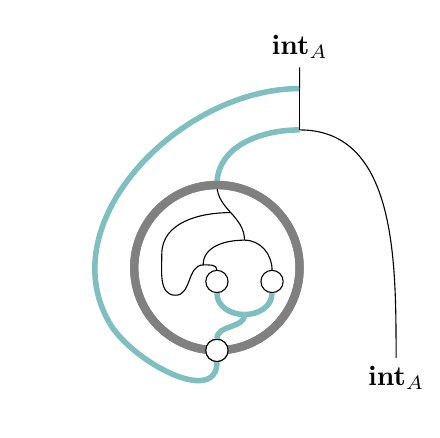
\begin{tikzpicture}[scale=0.35,auto,inner sep=1mm]
\coordinate (topr) at (0,2);
\coordinate (comp) at (3,4);
\drawbang[out=90,in=180] (topr) to (comp);
\drawprom (0,-1) ellipse (3cm and 3cm);
\dernode (bottomr) at (0,-4) {};

% -------- promoted 2 ---------
% All coordinates are relative to the composition vertex (o), which itself
% has its coordinates derived from topr. This is the only link to the outside namespace.
\coordinate (o) at ($ (topr) + (1,-2) $);
\coordinate (ellipse_center) at ($ (o) - (1,1) $);
\coordinate (elbow) at ($ (o) - (3, 0.5) $);
\coordinate (top_of_circle) at ($ (o) + (-1,2) $);
\draw[out=90,in=270] (o) to (top_of_circle);
\drawprom (ellipse_center) ellipse (3cm and 3cm); % outer boundary
\dernode (bottomr) at ($ (o) - (1,4) $) {};
\dernode (R) at ($ (o) + (1, -1.5) $) {}; % right dereliction
\dernode (L) at ($ (o) - (1,1.5) $) {}; % left dereliction
\coordinate (left_curve) at ($ (o) - (2.5,2) $);
\coordinate (left_meet) at ($ (o) - (1.5, 0.9) $);
\coordinate (delta) at ($ (o) - (0, 2.7) $); % coproduct vertex
\draw[out=90,in=0] (R) to node [swap] {} (o);
\drawbang[out=0,in=270] (delta) to (R);
\drawbang[out=180,in=270] (delta) to (L);
\drawbang[out=90,in=270] (bottomr) to (delta);
\draw[out=90,in=180] (left_meet) to (o);
\draw[out=90,in=0] (L) to (left_meet);
\draw[out=0,in=180] (left_curve) to (left_meet);
\draw[out=180,in=270] (left_curve) to (elbow);
\draw[out=90,in=180] (elbow) to ($ (o)!.5!(top_of_circle) $);
% ------ end promoted 2 ------

% Now for the rest of the diagram
\coordinate (curve) at (-3.9, -3);
\coordinate (meet) at (3,5.5);
\drawbang[out=300,in=270] (curve) to (bottomr);
\drawbang[out=120,in=180] (curve) to (meet);
\node (inta) at (6.5,-5) {$\inta_A$};
\draw[out=90,in=0] (inta) to (comp);
\node (vtop) at (3,7) {$\inta_A$};
\draw (meet) to (vtop);
\draw (comp) to (meet);
\end{tikzpicture}

&

\subsection{A sketch of future work}\label{section:sketch}

%However the connection we want to emphasise, and which will be elaborated further in \cite{??}, is between linear logic and algebraic geometry and higher categories. 

Proofs in linear logic naturally have shadows in contexts where there is an interaction between \emph{linear} objects and the \emph{non-linear} objects which classify them (e.g. vector bundles and moduli spaces of vector bundles). We have in mind the following kind of situation: let $\cat{B}$ be a bicategory which we think of as having algebraic spaces as objects and some kind of correspondences or integral transforms as $1$-morphisms. Two of the assumptions we make about this bicategory are:
\begin{itemize}
\item[(i)] It is symmetric monoidal and closed, so that for a pair of objects $v,w$ we may form $v \otimes w$ and $\Hom(v,w)$, and
\item[(ii)] for each pair of objects $v,w$ there is a reasonable moduli space $\mathscr{M}_{v,w}$ whose points are in bijection with $1$-morphisms $v \lto w$ in $\cat{B}$ and that these moduli spaces themselves form valid objects of $\cat{B}$.
\end{itemize}
What distinguishes $\mathscr{M}_{v,w}$ from $\Hom(v,w)$ is that the former is supposed to be ``space-like'' which means it is a coalgebra, i.e. comes equipped with natural $1$-morphisms $\mathscr{M}_{v,w} \lto \mathscr{M}_{v,w} \otimes \mathscr{M}_{v,w}$ and $\mathscr{M}_{v,w} \lto 1$. In for example the bicategory of smooth projective varieties every object is equipped with such $1$-morphisms, given by the diagonal and the graph of the structure map.

It therefore makes sense to ask for a ``universal'' $1$-morphism $\mathscr{M}_{v,w} \lto \Hom(v,w)$ whose value over a point $[X]$ of the moduli space corresponding to $X: v \lto w$ is $X$ itself.

In this situation we can expect to find a semantics of linear logic in the bicategory $\cat{B}$. For instance, if the formula $A$ of the logic is assigned the object $v$ of the bicategory, then the proof \eqref{church_2_intro} given above is represented by a $1$-morphism
\[
\mathscr{M}_{v,v} \lto \Hom(v,v)
\]
whose value over a point $[X]$ of $\mathscr{M}_{v,v}$ is the square $X \circ X$ of a loop $X: v \lto v$. In this way arbitrary integers, encoded as proofs in linear logic, may be represented as $1$-morphisms in $\cat{B}$, and the same is true any program computing integers from integers that can be encoded in linear logic. The remarkable thing is that all of this structure is immediately present as soon as we allow the objects $\Hom(v,w)$ to interact with their own moduli spaces. In \cite{??} and its forthcoming sequels this is made precise when $\cat{B}$ is a bicategory of matrix factorisations.

% What happens when we stabilise by ensuring that between any two objects there is always a generic? In a symmetric monoidal category we know how to enumerate all the "canonical" morphisms: they are terms in some language. What is the language that tells us how to enumerate all the canonical constructions that are possible in a setting such as the one we have just enumerated? That is, the structures that do not depend on the particular properties of matrix factorisations and are ``inherent'' in this notion of taking iterated moduli spaces? This language is linear logic.

% One should not underestimate the rapid progress in abstraction and uptake of academic ideas between computer science and industry. Maybe in a few decades it will be ordinary for Google employees to be programming with simplicial sets and Kan fibrations \cite{??}.
